\documentclass[a4paper]{tufte-handout}
\usepackage{pgfplots}
\usepackage[dvipsnames]{xcolor}
\usepackage{ulem}
\usepackage{subcaption}
\usepackage{amssymb, amsmath, pgfplots, tabularx, siunitx}
\usepackage{algorithm}
\usepackage{makecell}
\usepackage{amsfonts}
\pgfplotsset{compat = newest}

\usepackage{tikz}
\usetikzlibrary{shadings}
\usetikzlibrary{calc,arrows.meta}
\usetikzlibrary{shapes.misc}
\usetikzlibrary{positioning}
\usetikzlibrary{decorations.pathreplacing, shapes.geometric}
\usepackage[most]{tcolorbox}
\usepgfplotslibrary{colormaps,patchplots}

\definecolor{wp-bg}{HTML}{FDF6EF}
\definecolor{wp-text}{HTML}{2D1B0E}
\definecolor{wp-primary}{HTML}{C24A3A}
\definecolor{wp-accent}{HTML}{D4952E}
\definecolor{wp-light}{HTML}{F0DECA}
\definecolor{wp-muted}{HTML}{C4A88A}
\definecolor{wp-dark}{HTML}{1A0F07}
\definecolor{wp-code}{HTML}{FDF2E4}

\pagecolor{wp-bg}
\color{wp-text}

\hypersetup{colorlinks=true,linkcolor=wp-primary,urlcolor=wp-muted}

\graphicspath{{genai-imagen/cover/}{cover/}}

\makeatletter
\newcommand{\coverpage}{%
  \thispagestyle{empty}%
  \begin{tikzpicture}[remember picture, overlay]
    \fill[wp-bg] (current page.south west) rectangle (current page.north east);
    \node[inner sep=0] at (current page.center) {%
      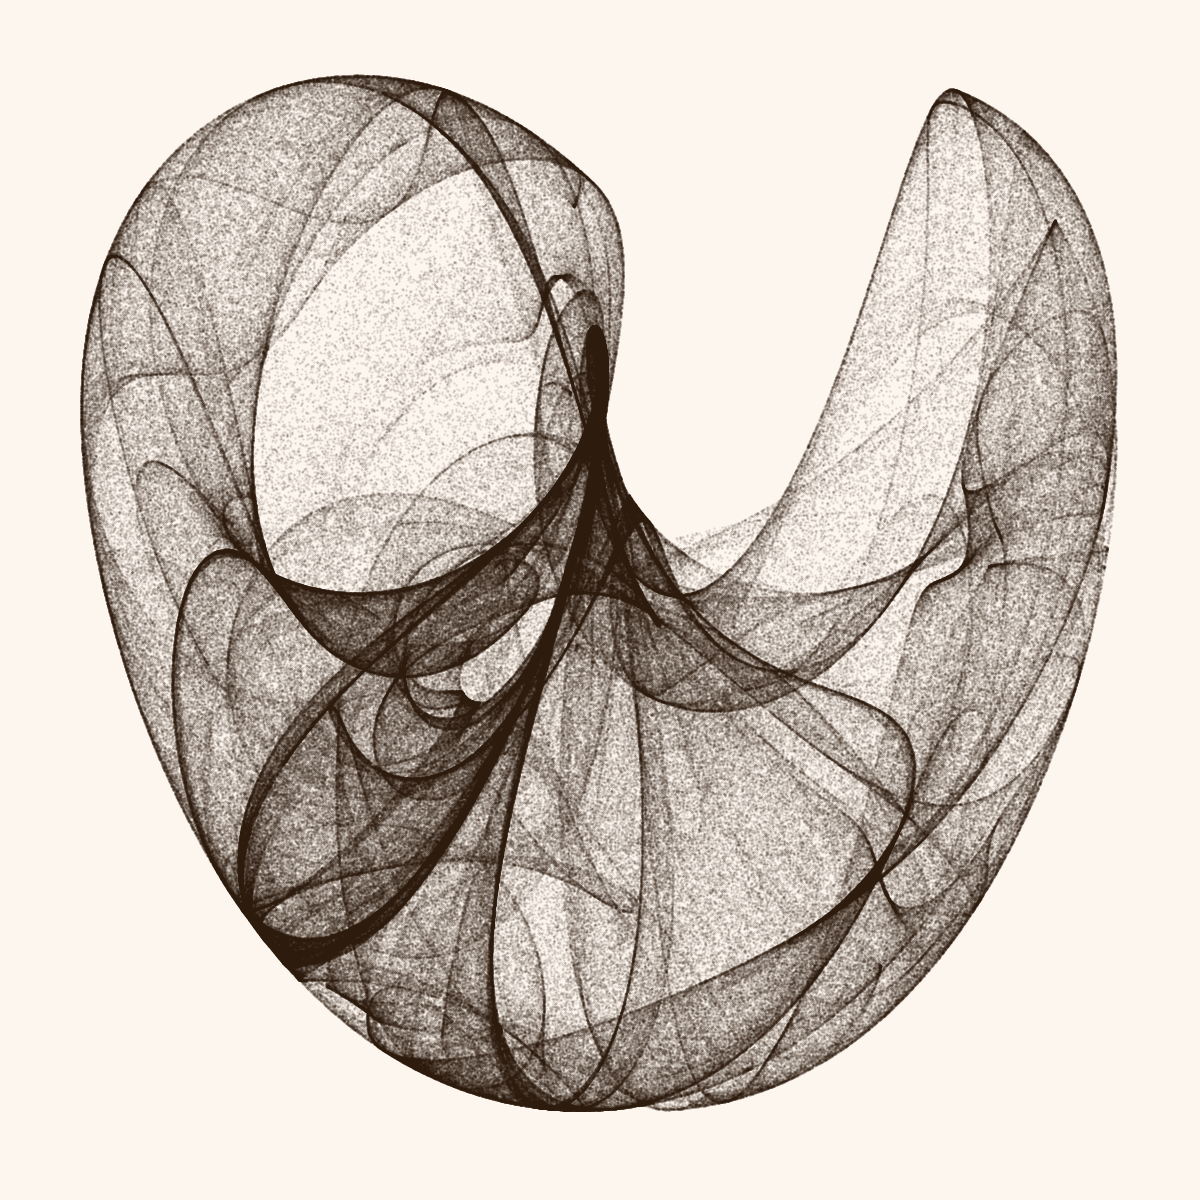
\includegraphics[width=0.9\textwidth]{attractor-image.png}%
    };
    \node[align=center, text=wp-text, yshift=-8cm, text width=0.90\paperwidth] at (current page.center) {%
      \bfseries\Huge \@title \\[0.5em]
      \normalsize \@author \\[0.5em]
      \normalsize \@date
    };
  \end{tikzpicture}%
}
\makeatother

\tikzset{basic/.style={draw,text width=1em,text badly centered}}
\tikzset{input/.style={basic,circle}}
\tikzset{weights/.style={basic,rectangle}}
\tikzset{functions/.style={basic,circle}}

\title{Introdução à Modelos Generativos para Imagem}
\author{Vitor N. Cabral de Oliveira\\ \href{mailto:vnco@cin.ufpe.br}{vnco@cin.ufpe.br}}

\date{\today}

\begin{document}

\coverpage
\newpage

\maketitle
\hypersetup{linkcolor=wp-primary}
\makeatletter
\def\input@path{{resources/style-transfer/}{resources/gan/}{../resources/style-transfer/}{../resources/gan/}}
\makeatother
\newpage
\hypersetup{linkcolor=wp-text}
\tableofcontents
\hypersetup{linkcolor=wp-primary}
\newpage

\section{Style Transfer}

A transferência de estilo é uma técnica de visão computacional que utiliza redes neurais convolucionais (CNNs) para gerar uma nova imagem que combina o conteúdo de uma imagem com o estilo artístico de outra. Essa técnica foi proposta no artigo seminal \textit{A Neural Algorithm of Artistic Style} por Leon Gatys et al. e faz uso de redes convolucionais pré-treinadas, como a ResNet50, para extrair características visuais de diferentes níveis de abstração.

A metodologia se baseia na relação entre as múltiplas camadas de uma CNN, onde cada camada $l$ produz um conjunto de mapas de características $F^{l}(I)$. Esses mapas capturam informações visuais em diferentes níveis de complexidade, desde bordas e texturas nas camadas iniciais até formas e objetos nas camadas mais profundas. Assim, a CNN pode ser vista como um extrator hierárquico de características, onde cada camada contribui para a representação da imagem $I$.

% Style Transfer — Hierarquia de Características na CNN (Grelha Corrigida)
% Uso: % Style Transfer — Hierarquia de Características na CNN (Grelha Corrigida)
% Uso: % Style Transfer — Hierarquia de Características na CNN (Grelha Corrigida)
% Uso: \input{resources/style-transfer/cnn-hierarchy.tex}
\begin{figure}[htbp]
\centering
\resizebox{\textwidth}{!}{%
\begin{tikzpicture}[
    >=latex,
    layer/.style={draw=wp-text, rounded corners=2pt, minimum width=3.0cm, minimum height=1.2cm, align=center, font=\small},
    conn/.style={->, draw=wp-primary, thick},
    brk/.style={decorate, decoration={brace, amplitude=5pt}, draw=wp-muted, thick},
    tuftebox/.style={draw=wp-light, fill=wp-code, rounded corners=2pt, align=center}
]

% =========================================================================
% FLUXO PRINCIPAL: CAMADAS DA CNN (Eixo X Otimizado)
% =========================================================================

\node[layer, fill=wp-accent!15, draw=wp-accent] (conv1) at (3.5, 2.5) {Camadas Iniciais\\conv$_1$ -- conv$_2$};
\node[layer, fill=wp-primary!10, draw=wp-primary] (conv2) at (7.0, 2.5) {Camadas Médias\\conv$_3$ -- conv$_4$};
\node[layer, fill=wp-text!10, draw=wp-text] (conv3) at (10.5, 2.5) {Camadas Profundas\\conv$_5$ -- conv$_6$};

% Imagem de Entrada simplificada para apenas "X"
\node[draw=wp-text, fill=wp-code, rounded corners=2pt, minimum width=1.0cm, minimum height=1.0cm, align=center, font=\large\bfseries] (input) at (0.8, 2.5) {$\mathcal{I}$};

% Conexões do Fluxo Principal
\draw[->, draw=wp-primary, thick] (input.east) -- (conv1.west);
\draw[->, draw=wp-primary, thick] (conv1.east) -- (conv2.west);
\draw[->, draw=wp-primary, thick] (conv2.east) -- (conv3.west);


% =========================================================================
% VISUALIZAÇÕES DE RECURSOS (Aproximadas verticalmente)
% =========================================================================

\node (vis1) at (3.5, 1.1) {
  \begin{tikzpicture}[scale=0.3]
    \foreach \i in {0,...,4}
      \foreach \j in {0,...,4}
        \pgfmathparse{mod(\i+\j,2)*100}
        \fill[black!\pgfmathresult] (\i*0.5, -\j*0.5) rectangle ++(0.45, 0.45);
  \end{tikzpicture}\quad
  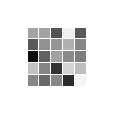
\begin{tikzpicture}[scale=0.3]
    \foreach \i in {0,...,4}
      \foreach \j in {0,...,4}
        \pgfmathparse{int(rnd*100)}
        \fill[black!\pgfmathresult] (\i*0.5, -\j*0.5) rectangle ++(0.45, 0.45);
  \end{tikzpicture}\quad
  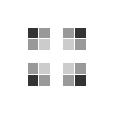
\begin{tikzpicture}[scale=0.3]
    \foreach \i in {0,...,4}
      \foreach \j in {0,...,4}
        \pgfmathparse{abs(\i-2)*abs(\j-2)*20}
        \fill[black!\pgfmathresult] (\i*0.5, -\j*0.5) rectangle ++(0.45, 0.45);
  \end{tikzpicture}
};

\node (vis2) at (7.0, 1.1) {
  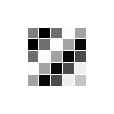
\begin{tikzpicture}[scale=0.3]
    \foreach \i in {0,...,4}
      \foreach \j in {0,...,4}
        \pgfmathparse{sin(deg(\i*1.5+\j*1.5))*50+50}
        \fill[black!\pgfmathresult] (\i*0.5, -\j*0.5) rectangle ++(0.45, 0.45);
  \end{tikzpicture}\quad
  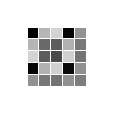
\begin{tikzpicture}[scale=0.3]
    \foreach \i in {0,...,4}
      \foreach \j in {0,...,4}
        \pgfmathparse{cos(deg(\i*2))*cos(deg(\j*2))*50+50}
        \fill[black!\pgfmathresult] (\i*0.5, -\j*0.5) rectangle ++(0.45, 0.45);
  \end{tikzpicture}\quad
  
\begin{tikzpicture}[scale=0.3]
    \foreach \i in {0,...,4}
      \foreach \j in {0,...,4}
        \pgfmathparse{sin(deg(sqrt(\i^2+\j^2)*2))*50+50}
        \fill[black!\pgfmathresult] (\i*0.5, -\j*0.5) rectangle ++(0.45, 0.45);
  \end{tikzpicture}
};

\node (vis3) at (10.5, 1.1) {
  
\begin{tikzpicture}[scale=0.3]
    \foreach \i in {0,...,4}
      \foreach \j in {0,...,4}
        \pgfmathparse{\i==2 && \j==2 ? 80 : 10}
        \fill[black!\pgfmathresult] (\i*0.5, -\j*0.5) rectangle ++(0.45, 0.45);
  \end{tikzpicture}\quad
  
\begin{tikzpicture}[scale=0.3]
    \foreach \i in {0,...,4}
      \foreach \j in {0,...,4}
        \pgfmathparse{(\i-2)^2+(\j-2)^2 < 2 ? 80 : 10}
        \fill[black!\pgfmathresult] (\i*0.5, -\j*0.5) rectangle ++(0.45, 0.45);
  \end{tikzpicture}\quad
  
\begin{tikzpicture}[scale=0.3]
    \foreach \i in {0,...,4}
      \foreach \j in {0,...,4}
        \pgfmathparse{(\i==1 || \i==3) && (\j>=1 && \j<=3) ? 80 : 10}
        \fill[black!\pgfmathresult] (\i*0.5, -\j*0.5) rectangle ++(0.45, 0.45);
  \end{tikzpicture}
};

% --- SETAS PONTILHADAS ---
\draw[->, draw=wp-muted, thick, dashed] (conv1.south) -- (vis1.north);
\draw[->, draw=wp-muted, thick, dashed] (conv2.south) -- (vis2.north);
\draw[->, draw=wp-muted, thick, dashed] (conv3.south) -- (vis3.north);


% --- TEXTOS INFERIORES DE CARACTERÍSTICAS ---
\node[font=\footnotesize, align=center, text=wp-accent] at (3.5, -0.1) {Bordas\\Texturas\\Cores};
\node[font=\footnotesize, align=center, text=wp-primary] at (7.0, -0.1) {Padrões\\Partes\\Formas simples};
\node[font=\footnotesize, align=center, text=wp-text] at (10.5, -0.1) {Objetos\\Semântica\\Conceitos};


% --- CHAVES SUPERIORES (Braces) ---
\draw[brk] (5.1, 4.0) -- (1.9, 4.0);
\node[above=4pt, font=\small, text=wp-accent] at (3.5, 4.0) {ESTILO (baixo nível)};

\draw[brk] (8.6, 4.0) -- (5.4, 4.0);
\node[above=4pt, font=\small, text=wp-primary] at (7.0, 4.0) {transição};

\draw[brk] (12.1, 4.0) -- (8.9, 4.0);
\node[above=4pt, font=\small, text=wp-text] at (10.5, 4.0) {CONTEÚDO (alto nível)};


% =========================================================================
% BLOCO SUPERIOR RE-ALINHADO E PROPORCIONAL
% Centrado exatamente em x=7.0 (meio do gráfico) com largura equilibrada de 7.0cm
% =========================================================================
\node[tuftebox, minimum width=7.0cm, minimum height=1.2cm] at (7.0, 6.0) {
    \textbf{\color{wp-primary}\small Extração de Características e Perdas}\\[4pt]
    \footnotesize Perda de estilo: múltiplas camadas (baixo + médio)\\
    \footnotesize Perda de conteúdo: camada profunda (alto nível)
};

\end{tikzpicture}
}
\caption{Hierarquia de características em uma CNN. Camadas iniciais capturam bordas, texturas e cores (estilo). Camadas médias detectam padrões e partes de objetos. Camadas profundas representam objetos completos e semântica de alto nível (conteúdo). A perda de estilo utiliza múltiplas camadas iniciais e médias, enquanto a perda de conteúdo utiliza uma camada profunda.}
\label{fig:cnn-hierarchy}
\end{figure}
\begin{figure}[htbp]
\centering
\resizebox{\textwidth}{!}{%
\begin{tikzpicture}[
    >=latex,
    layer/.style={draw=wp-text, rounded corners=2pt, minimum width=3.0cm, minimum height=1.2cm, align=center, font=\small},
    conn/.style={->, draw=wp-primary, thick},
    brk/.style={decorate, decoration={brace, amplitude=5pt}, draw=wp-muted, thick},
    tuftebox/.style={draw=wp-light, fill=wp-code, rounded corners=2pt, align=center}
]

% =========================================================================
% FLUXO PRINCIPAL: CAMADAS DA CNN (Eixo X Otimizado)
% =========================================================================

\node[layer, fill=wp-accent!15, draw=wp-accent] (conv1) at (3.5, 2.5) {Camadas Iniciais\\conv$_1$ -- conv$_2$};
\node[layer, fill=wp-primary!10, draw=wp-primary] (conv2) at (7.0, 2.5) {Camadas Médias\\conv$_3$ -- conv$_4$};
\node[layer, fill=wp-text!10, draw=wp-text] (conv3) at (10.5, 2.5) {Camadas Profundas\\conv$_5$ -- conv$_6$};

% Imagem de Entrada simplificada para apenas "X"
\node[draw=wp-text, fill=wp-code, rounded corners=2pt, minimum width=1.0cm, minimum height=1.0cm, align=center, font=\large\bfseries] (input) at (0.8, 2.5) {$\mathcal{I}$};

% Conexões do Fluxo Principal
\draw[->, draw=wp-primary, thick] (input.east) -- (conv1.west);
\draw[->, draw=wp-primary, thick] (conv1.east) -- (conv2.west);
\draw[->, draw=wp-primary, thick] (conv2.east) -- (conv3.west);


% =========================================================================
% VISUALIZAÇÕES DE RECURSOS (Aproximadas verticalmente)
% =========================================================================

\node (vis1) at (3.5, 1.1) {
  \begin{tikzpicture}[scale=0.3]
    \foreach \i in {0,...,4}
      \foreach \j in {0,...,4}
        \pgfmathparse{mod(\i+\j,2)*100}
        \fill[black!\pgfmathresult] (\i*0.5, -\j*0.5) rectangle ++(0.45, 0.45);
  \end{tikzpicture}\quad
  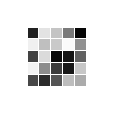
\begin{tikzpicture}[scale=0.3]
    \foreach \i in {0,...,4}
      \foreach \j in {0,...,4}
        \pgfmathparse{int(rnd*100)}
        \fill[black!\pgfmathresult] (\i*0.5, -\j*0.5) rectangle ++(0.45, 0.45);
  \end{tikzpicture}\quad
  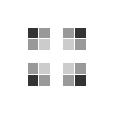
\begin{tikzpicture}[scale=0.3]
    \foreach \i in {0,...,4}
      \foreach \j in {0,...,4}
        \pgfmathparse{abs(\i-2)*abs(\j-2)*20}
        \fill[black!\pgfmathresult] (\i*0.5, -\j*0.5) rectangle ++(0.45, 0.45);
  \end{tikzpicture}
};

\node (vis2) at (7.0, 1.1) {
  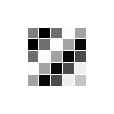
\begin{tikzpicture}[scale=0.3]
    \foreach \i in {0,...,4}
      \foreach \j in {0,...,4}
        \pgfmathparse{sin(deg(\i*1.5+\j*1.5))*50+50}
        \fill[black!\pgfmathresult] (\i*0.5, -\j*0.5) rectangle ++(0.45, 0.45);
  \end{tikzpicture}\quad
  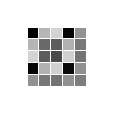
\begin{tikzpicture}[scale=0.3]
    \foreach \i in {0,...,4}
      \foreach \j in {0,...,4}
        \pgfmathparse{cos(deg(\i*2))*cos(deg(\j*2))*50+50}
        \fill[black!\pgfmathresult] (\i*0.5, -\j*0.5) rectangle ++(0.45, 0.45);
  \end{tikzpicture}\quad
  
\begin{tikzpicture}[scale=0.3]
    \foreach \i in {0,...,4}
      \foreach \j in {0,...,4}
        \pgfmathparse{sin(deg(sqrt(\i^2+\j^2)*2))*50+50}
        \fill[black!\pgfmathresult] (\i*0.5, -\j*0.5) rectangle ++(0.45, 0.45);
  \end{tikzpicture}
};

\node (vis3) at (10.5, 1.1) {
  
\begin{tikzpicture}[scale=0.3]
    \foreach \i in {0,...,4}
      \foreach \j in {0,...,4}
        \pgfmathparse{\i==2 && \j==2 ? 80 : 10}
        \fill[black!\pgfmathresult] (\i*0.5, -\j*0.5) rectangle ++(0.45, 0.45);
  \end{tikzpicture}\quad
  
\begin{tikzpicture}[scale=0.3]
    \foreach \i in {0,...,4}
      \foreach \j in {0,...,4}
        \pgfmathparse{(\i-2)^2+(\j-2)^2 < 2 ? 80 : 10}
        \fill[black!\pgfmathresult] (\i*0.5, -\j*0.5) rectangle ++(0.45, 0.45);
  \end{tikzpicture}\quad
  
\begin{tikzpicture}[scale=0.3]
    \foreach \i in {0,...,4}
      \foreach \j in {0,...,4}
        \pgfmathparse{(\i==1 || \i==3) && (\j>=1 && \j<=3) ? 80 : 10}
        \fill[black!\pgfmathresult] (\i*0.5, -\j*0.5) rectangle ++(0.45, 0.45);
  \end{tikzpicture}
};

% --- SETAS PONTILHADAS ---
\draw[->, draw=wp-muted, thick, dashed] (conv1.south) -- (vis1.north);
\draw[->, draw=wp-muted, thick, dashed] (conv2.south) -- (vis2.north);
\draw[->, draw=wp-muted, thick, dashed] (conv3.south) -- (vis3.north);


% --- TEXTOS INFERIORES DE CARACTERÍSTICAS ---
\node[font=\footnotesize, align=center, text=wp-accent] at (3.5, -0.1) {Bordas\\Texturas\\Cores};
\node[font=\footnotesize, align=center, text=wp-primary] at (7.0, -0.1) {Padrões\\Partes\\Formas simples};
\node[font=\footnotesize, align=center, text=wp-text] at (10.5, -0.1) {Objetos\\Semântica\\Conceitos};


% --- CHAVES SUPERIORES (Braces) ---
\draw[brk] (5.1, 4.0) -- (1.9, 4.0);
\node[above=4pt, font=\small, text=wp-accent] at (3.5, 4.0) {ESTILO (baixo nível)};

\draw[brk] (8.6, 4.0) -- (5.4, 4.0);
\node[above=4pt, font=\small, text=wp-primary] at (7.0, 4.0) {transição};

\draw[brk] (12.1, 4.0) -- (8.9, 4.0);
\node[above=4pt, font=\small, text=wp-text] at (10.5, 4.0) {CONTEÚDO (alto nível)};


% =========================================================================
% BLOCO SUPERIOR RE-ALINHADO E PROPORCIONAL
% Centrado exatamente em x=7.0 (meio do gráfico) com largura equilibrada de 7.0cm
% =========================================================================
\node[tuftebox, minimum width=7.0cm, minimum height=1.2cm] at (7.0, 6.0) {
    \textbf{\color{wp-primary}\small Extração de Características e Perdas}\\[4pt]
    \footnotesize Perda de estilo: múltiplas camadas (baixo + médio)\\
    \footnotesize Perda de conteúdo: camada profunda (alto nível)
};

\end{tikzpicture}
}
\caption{Hierarquia de características em uma CNN. Camadas iniciais capturam bordas, texturas e cores (estilo). Camadas médias detectam padrões e partes de objetos. Camadas profundas representam objetos completos e semântica de alto nível (conteúdo). A perda de estilo utiliza múltiplas camadas iniciais e médias, enquanto a perda de conteúdo utiliza uma camada profunda.}
\label{fig:cnn-hierarchy}
\end{figure}
\begin{figure}[htbp]
\centering
\resizebox{\textwidth}{!}{%
\begin{tikzpicture}[
    >=latex,
    layer/.style={draw=wp-text, rounded corners=2pt, minimum width=3.0cm, minimum height=1.2cm, align=center, font=\small},
    conn/.style={->, draw=wp-primary, thick},
    brk/.style={decorate, decoration={brace, amplitude=5pt}, draw=wp-muted, thick},
    tuftebox/.style={draw=wp-light, fill=wp-code, rounded corners=2pt, align=center}
]

% =========================================================================
% FLUXO PRINCIPAL: CAMADAS DA CNN (Eixo X Otimizado)
% =========================================================================

\node[layer, fill=wp-accent!15, draw=wp-accent] (conv1) at (3.5, 2.5) {Camadas Iniciais\\conv$_1$ -- conv$_2$};
\node[layer, fill=wp-primary!10, draw=wp-primary] (conv2) at (7.0, 2.5) {Camadas Médias\\conv$_3$ -- conv$_4$};
\node[layer, fill=wp-text!10, draw=wp-text] (conv3) at (10.5, 2.5) {Camadas Profundas\\conv$_5$ -- conv$_6$};

% Imagem de Entrada simplificada para apenas "X"
\node[draw=wp-text, fill=wp-code, rounded corners=2pt, minimum width=1.0cm, minimum height=1.0cm, align=center, font=\large\bfseries] (input) at (0.8, 2.5) {$\mathcal{I}$};

% Conexões do Fluxo Principal
\draw[->, draw=wp-primary, thick] (input.east) -- (conv1.west);
\draw[->, draw=wp-primary, thick] (conv1.east) -- (conv2.west);
\draw[->, draw=wp-primary, thick] (conv2.east) -- (conv3.west);


% =========================================================================
% VISUALIZAÇÕES DE RECURSOS (Aproximadas verticalmente)
% =========================================================================

\node (vis1) at (3.5, 1.1) {
  \begin{tikzpicture}[scale=0.3]
    \foreach \i in {0,...,4}
      \foreach \j in {0,...,4}
        \pgfmathparse{mod(\i+\j,2)*100}
        \fill[black!\pgfmathresult] (\i*0.5, -\j*0.5) rectangle ++(0.45, 0.45);
  \end{tikzpicture}\quad
  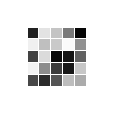
\begin{tikzpicture}[scale=0.3]
    \foreach \i in {0,...,4}
      \foreach \j in {0,...,4}
        \pgfmathparse{int(rnd*100)}
        \fill[black!\pgfmathresult] (\i*0.5, -\j*0.5) rectangle ++(0.45, 0.45);
  \end{tikzpicture}\quad
  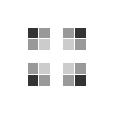
\begin{tikzpicture}[scale=0.3]
    \foreach \i in {0,...,4}
      \foreach \j in {0,...,4}
        \pgfmathparse{abs(\i-2)*abs(\j-2)*20}
        \fill[black!\pgfmathresult] (\i*0.5, -\j*0.5) rectangle ++(0.45, 0.45);
  \end{tikzpicture}
};

\node (vis2) at (7.0, 1.1) {
  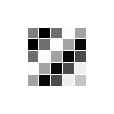
\begin{tikzpicture}[scale=0.3]
    \foreach \i in {0,...,4}
      \foreach \j in {0,...,4}
        \pgfmathparse{sin(deg(\i*1.5+\j*1.5))*50+50}
        \fill[black!\pgfmathresult] (\i*0.5, -\j*0.5) rectangle ++(0.45, 0.45);
  \end{tikzpicture}\quad
  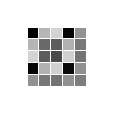
\begin{tikzpicture}[scale=0.3]
    \foreach \i in {0,...,4}
      \foreach \j in {0,...,4}
        \pgfmathparse{cos(deg(\i*2))*cos(deg(\j*2))*50+50}
        \fill[black!\pgfmathresult] (\i*0.5, -\j*0.5) rectangle ++(0.45, 0.45);
  \end{tikzpicture}\quad
  
\begin{tikzpicture}[scale=0.3]
    \foreach \i in {0,...,4}
      \foreach \j in {0,...,4}
        \pgfmathparse{sin(deg(sqrt(\i^2+\j^2)*2))*50+50}
        \fill[black!\pgfmathresult] (\i*0.5, -\j*0.5) rectangle ++(0.45, 0.45);
  \end{tikzpicture}
};

\node (vis3) at (10.5, 1.1) {
  
\begin{tikzpicture}[scale=0.3]
    \foreach \i in {0,...,4}
      \foreach \j in {0,...,4}
        \pgfmathparse{\i==2 && \j==2 ? 80 : 10}
        \fill[black!\pgfmathresult] (\i*0.5, -\j*0.5) rectangle ++(0.45, 0.45);
  \end{tikzpicture}\quad
  
\begin{tikzpicture}[scale=0.3]
    \foreach \i in {0,...,4}
      \foreach \j in {0,...,4}
        \pgfmathparse{(\i-2)^2+(\j-2)^2 < 2 ? 80 : 10}
        \fill[black!\pgfmathresult] (\i*0.5, -\j*0.5) rectangle ++(0.45, 0.45);
  \end{tikzpicture}\quad
  
\begin{tikzpicture}[scale=0.3]
    \foreach \i in {0,...,4}
      \foreach \j in {0,...,4}
        \pgfmathparse{(\i==1 || \i==3) && (\j>=1 && \j<=3) ? 80 : 10}
        \fill[black!\pgfmathresult] (\i*0.5, -\j*0.5) rectangle ++(0.45, 0.45);
  \end{tikzpicture}
};

% --- SETAS PONTILHADAS ---
\draw[->, draw=wp-muted, thick, dashed] (conv1.south) -- (vis1.north);
\draw[->, draw=wp-muted, thick, dashed] (conv2.south) -- (vis2.north);
\draw[->, draw=wp-muted, thick, dashed] (conv3.south) -- (vis3.north);


% --- TEXTOS INFERIORES DE CARACTERÍSTICAS ---
\node[font=\footnotesize, align=center, text=wp-accent] at (3.5, -0.1) {Bordas\\Texturas\\Cores};
\node[font=\footnotesize, align=center, text=wp-primary] at (7.0, -0.1) {Padrões\\Partes\\Formas simples};
\node[font=\footnotesize, align=center, text=wp-text] at (10.5, -0.1) {Objetos\\Semântica\\Conceitos};


% --- CHAVES SUPERIORES (Braces) ---
\draw[brk] (5.1, 4.0) -- (1.9, 4.0);
\node[above=4pt, font=\small, text=wp-accent] at (3.5, 4.0) {ESTILO (baixo nível)};

\draw[brk] (8.6, 4.0) -- (5.4, 4.0);
\node[above=4pt, font=\small, text=wp-primary] at (7.0, 4.0) {transição};

\draw[brk] (12.1, 4.0) -- (8.9, 4.0);
\node[above=4pt, font=\small, text=wp-text] at (10.5, 4.0) {CONTEÚDO (alto nível)};


% =========================================================================
% BLOCO SUPERIOR RE-ALINHADO E PROPORCIONAL
% Centrado exatamente em x=7.0 (meio do gráfico) com largura equilibrada de 7.0cm
% =========================================================================
\node[tuftebox, minimum width=7.0cm, minimum height=1.2cm] at (7.0, 6.0) {
    \textbf{\color{wp-primary}\small Extração de Características e Perdas}\\[4pt]
    \footnotesize Perda de estilo: múltiplas camadas (baixo + médio)\\
    \footnotesize Perda de conteúdo: camada profunda (alto nível)
};

\end{tikzpicture}
}
\caption{Hierarquia de características em uma CNN. Camadas iniciais capturam bordas, texturas e cores (estilo). Camadas médias detectam padrões e partes de objetos. Camadas profundas representam objetos completos e semântica de alto nível (conteúdo). A perda de estilo utiliza múltiplas camadas iniciais e médias, enquanto a perda de conteúdo utiliza uma camada profunda.}
\label{fig:cnn-hierarchy}
\end{figure}

O processo de transferência de estilo depende de duas imagens de entrada:
\begin{enumerate}
    \item \textbf{Imagem de conteúdo ($C$)}: Contém a estrutura e os objetos principais que serão preservados na imagem gerada.
    \item \textbf{Imagem de estilo ($S$)}: Fornece as texturas, cores e padrões artísticos que serão transferidos para a imagem final.
\end{enumerate}


A imagem gerada ($G$) é obtida por meio da otimização de uma função de perda composta, que combina a representação do conteúdo e do estilo.

% Style Transfer — Pipeline completo (Grelha e Alinhamento Otimizados)
% Uso: % Style Transfer — Pipeline completo (Grelha e Alinhamento Otimizados)
% Uso: % Style Transfer — Pipeline completo (Grelha e Alinhamento Otimizados)
% Uso: \input{resources/style-transfer/style-transfer-pipeline.tex}
\begin{figure*}[htbp]
\centering
\resizebox{\textwidth}{!}{%
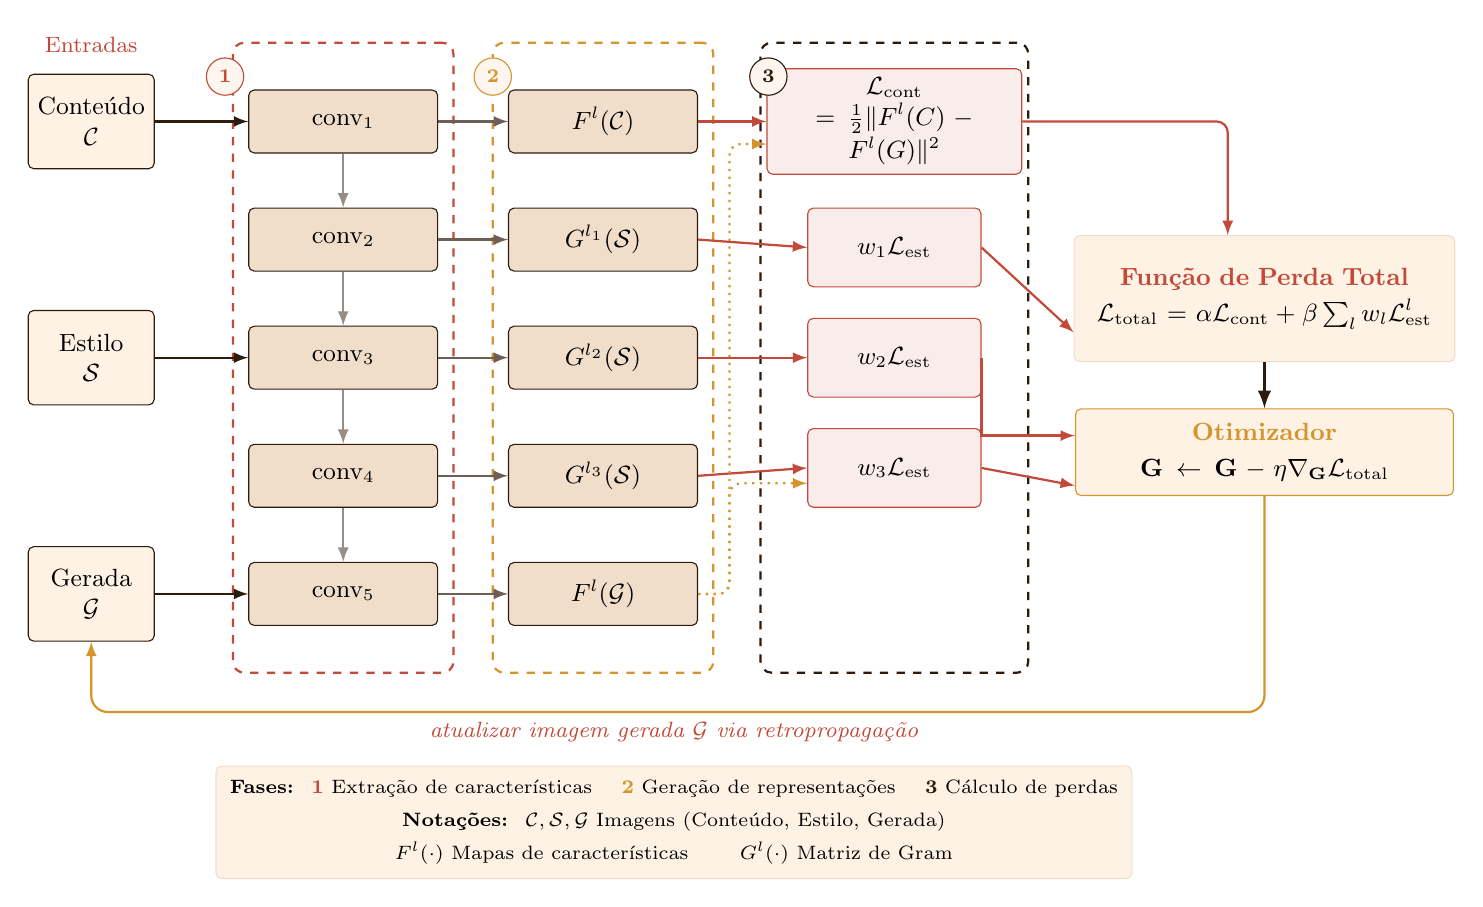
\begin{tikzpicture}[
    >=latex,
    box/.style={draw=wp-text, fill=wp-light, rounded corners=2pt, minimum width=2.4cm, minimum height=0.8cm, align=center, font=\small},
    img/.style={draw=wp-text, fill=wp-code, rounded corners=2pt, minimum width=1.6cm, minimum height=1.2cm, align=center, font=\small},
    loss/.style={draw=wp-primary, fill=wp-primary!10, rounded corners=2pt, minimum width=2.2cm, minimum height=1.0cm, align=center, font=\small},
    cnn/.style={draw=wp-primary, dashed, line width=0.8pt, fill=none, rounded corners=4pt, minimum width=2.8cm, minimum height=8cm, align=center, font=\small},
    grambox/.style={draw=wp-accent, dashed, line width=0.8pt, fill=none, rounded corners=4pt, minimum width=2.8cm, minimum height=8cm, align=center, font=\small},
    lossbox/.style={draw=wp-text, dashed, line width=0.8pt, fill=none, rounded corners=4pt, minimum width=3.4cm, minimum height=8cm, align=center, font=\small},
    conn/.style={->, draw=wp-primary, thick},
    label/.style={font=\footnotesize, text=wp-primary},
    tuftebox/.style={draw=wp-light, fill=wp-code, rounded corners=2pt, align=center}
]

% =========================================================================
% ENTRADAS: TENSORES DE IMAGEM SIMPLIFICADOS
% =========================================================================
\node[img] (content) at (0, 3.0)  {Conteúdo\\$\mathcal{C}$};
\node[img] (style)   at (0, 0.0)  {Estilo\\$\mathcal{S}$};
\node[img] (gen)     at (0, -3.0) {Gerada\\$\mathcal{G}$};

\node[label, above=4.2pt] at (content.north) {Entradas};

% =========================================================================
% CAMADAS DA CNN (Fase 1 - Container unificado)
% =========================================================================
\node[cnn] (cnn_box) at (3.2, 0) {};

\node[box] (conv1) at (3.2, 3.0)  {conv$_1$};
\node[box] (conv2) at (3.2, 1.5)  {conv$_2$};
\node[box] (conv3) at (3.2, 0.0)  {conv$_3$};
\node[box] (conv4) at (3.2, -1.5) {conv$_4$};
\node[box] (conv5) at (3.2, -3.0) {conv$_5$};

% Fluxo interno da CNN
\draw[->, draw=wp-text!50, thick] (conv1) -- (conv2);
\draw[->, draw=wp-text!50, thick] (conv2) -- (conv3);
\draw[->, draw=wp-text!50, thick] (conv3) -- (conv4);
\draw[->, draw=wp-text!50, thick] (conv4) -- (conv5);

% Conexões das entradas para a CNN
\draw[->, draw=wp-text, thick] (content.east) -- (conv1.west);
\draw[->, draw=wp-text, thick] (style.east)   -- (conv3.west);
\draw[->, draw=wp-text, thick] (gen.east)     -- (conv5.west);


% =========================================================================
% MAPAS DE CARACTERÍSTICAS E MATRIZES DE GRAM (Fase 2)
% =========================================================================
\node[grambox] (gram_container) at (6.5, 0) {};

\node[box] (fm_c)  at (6.5,  3.0) {$F^l(\mathcal{C})$};
\node[box] (gm_s1) at (6.5,  1.5) {$G^{l_1}(\mathcal{S})$};
\node[box] (gm_s2) at (6.5,  0.0) {$G^{l_2}(\mathcal{S})$};
\node[box] (gm_s3) at (6.5, -1.5) {$G^{l_3}(\mathcal{S})$};
\node[box] (fm_g)  at (6.5, -3.0) {$F^l(\mathcal{G})$};

\draw[->, draw=wp-text!70, thick] (conv1.east) -- (fm_c.west);
\draw[->, draw=wp-text!70, thick] (conv2.east) -- (gm_s1.west);
\draw[->, draw=wp-text!70, thick] (conv3.east) -- (gm_s2.west);
\draw[->, draw=wp-text!70, thick] (conv4.east) -- (gm_s3.west);
\draw[->, draw=wp-text!70, thick] (conv5.east) -- (fm_g.west);


% =========================================================================
% COMPUTAÇÃO DE PERDAS (Fase 3)
% =========================================================================
\node[lossbox] (loss_container) at (10.2, 0) {};

\node[loss, text width=3.0cm] (l_c) at (10.2, 3.0) {$\mathcal{L}_{\mathrm{cont}}$\\$=\frac{1}{2}\|F^l(C)-F^l(G)\|^2$};
\node[loss] (l_s1) at (10.2,  1.4) {$w_1\mathcal{L}_{\mathrm{est}}$};
\node[loss] (l_s2) at (10.2,  0.0) {$w_2\mathcal{L}_{\mathrm{est}}$};
\node[loss] (l_s3) at (10.2, -1.4) {$w_3\mathcal{L}_{\mathrm{est}}$};

\draw[conn] (fm_c.east)  -- (l_c.west);
\draw[conn] (gm_s1.east) -- (l_s1.west);
\draw[conn] (gm_s2.east) -- (l_s2.west);
\draw[conn] (gm_s3.east) -- (l_s3.west);

% Feedback do G para as perdas
\draw[->, draw=wp-accent, thick, dotted, rounded corners=4pt] (fm_g.east) -- ++(0.4,0) |- (l_c.190);
\draw[->, draw=wp-accent, thick, dotted, rounded corners=4pt] (fm_g.east) -- ++(0.4,0) |- (l_s3.190);


% =========================================================================
% FUNÇÃO DE PERDA TOTAL & OTIMIZADOR
% =========================================================================
\node[tuftebox, minimum width=4.8cm, minimum height=1.6cm, text width=4.6cm, font=\small] (l_total) at (14.9, 0.75) {
    \textbf{\color{wp-primary}Função de Perda Total}\\[2pt] 
    $\mathcal{L}_{\mathrm{total}} = \alpha\mathcal{L}_{\mathrm{cont}} + \beta\sum_l w_l\mathcal{L}_{\mathrm{est}}^l$
};

\node[draw=wp-accent, fill=wp-code, rounded corners=2pt, minimum width=4.8cm, minimum height=1.1cm, text width=4.2cm, font=\small, align=center] (opt) at (14.9, -1.2) {
    \textbf{\color{wp-accent}Otimizador}\\[2pt] 
    $\mathbf{G} \leftarrow \mathbf{G} - \eta\nabla_{\mathbf{G}}\mathcal{L}_{\mathrm{total}}$
};

% Conexões para a direita
\draw[->, draw=wp-primary, thick, rounded corners=4pt] (l_c.east) -| (l_total.120);
\draw[->, draw=wp-primary, thick] (l_s1.east) -- (l_total.190);
\draw[->, draw=wp-primary, thick] (l_s2.east) |- (opt.175);
\draw[->, draw=wp-primary, thick] (l_s3.east) -- (opt.190);

\draw[->, draw=wp-text, very thick] (l_total.south) -- (opt.north);


% =========================================================================
% FASES DE PROCESSAMENTO (Indicadores Numéricos)
% =========================================================================
\node[draw=wp-primary, fill=wp-bg, circle, inner sep=2.5pt, font=\scriptsize\bfseries, text=wp-primary] at (1.7, 3.57) {1};
\node[draw=wp-accent, fill=wp-bg, circle, inner sep=2.5pt, font=\scriptsize\bfseries, text=wp-accent] at (5.1, 3.57) {2};
\node[draw=wp-text, fill=wp-bg, circle, inner sep=2.5pt, font=\scriptsize\bfseries, text=wp-text] at (8.6, 3.57) {3};


% =========================================================================
% FEEDBACK LOOP (Passando horizontalmente por baixo)
% =========================================================================
\draw[->, draw=wp-accent, thick, rounded corners=6pt] 
    (opt.south) -- (14.9, -4.5) -- (0, -4.5) -- (gen.south);

\node[label, font=\itshape\footnotesize, anchor=north] at (7.4, -4.5) 
    {atualizar imagem gerada $\mathcal{G}$ via retropropagação};


% =========================================================================
% LEGENDA DAS FASES E NOTAÇÕES REPOSICIONADA
% =========================================================================
\node[tuftebox, minimum width=10.0cm, minimum height=1.0cm, inner sep=5pt] (legenda) at (7.4, -5.9) {
    \scriptsize 
    \textbf{Fases:} \ 
    \textbf{\color{wp-primary}1} Extração de características \quad 
    \textbf{\color{wp-accent}2} Geração de representações \quad 
    \textbf{\color{wp-text}3} Cálculo de perdas \\
    \scriptsize
    \textbf{Notações:} \ 
    $\mathcal{C}, \mathcal{S}, \mathcal{G}$ Imagens (Conteúdo, Estilo, Gerada)\\
    \scriptsize
    $F^l(\cdot)$ Mapas de características \qquad 
    $G^l(\cdot)$ Matriz de Gram
};

\end{tikzpicture}
}
\caption{Pipeline completo de Style Transfer. Três imagens ($\mathcal{C}$, $\mathcal{S}$, $\mathcal{G}$) passam por uma CNN pré-treinada. Mapas de características de $\mathcal{C}$ e $\mathcal{G}$ em uma camada profunda definem a perda de conteúdo. Matrizes de Gram de $\mathcal{S}$ e $\mathcal{G}$ em múltiplos níveis definem a perda de estilo. A perda total é minimizada via gradiente descendente, atualizando $\mathcal{G}$.}
\label{fig:style-transfer-pipeline}
\end{figure*}
\begin{figure*}[htbp]
\centering
\resizebox{\textwidth}{!}{%
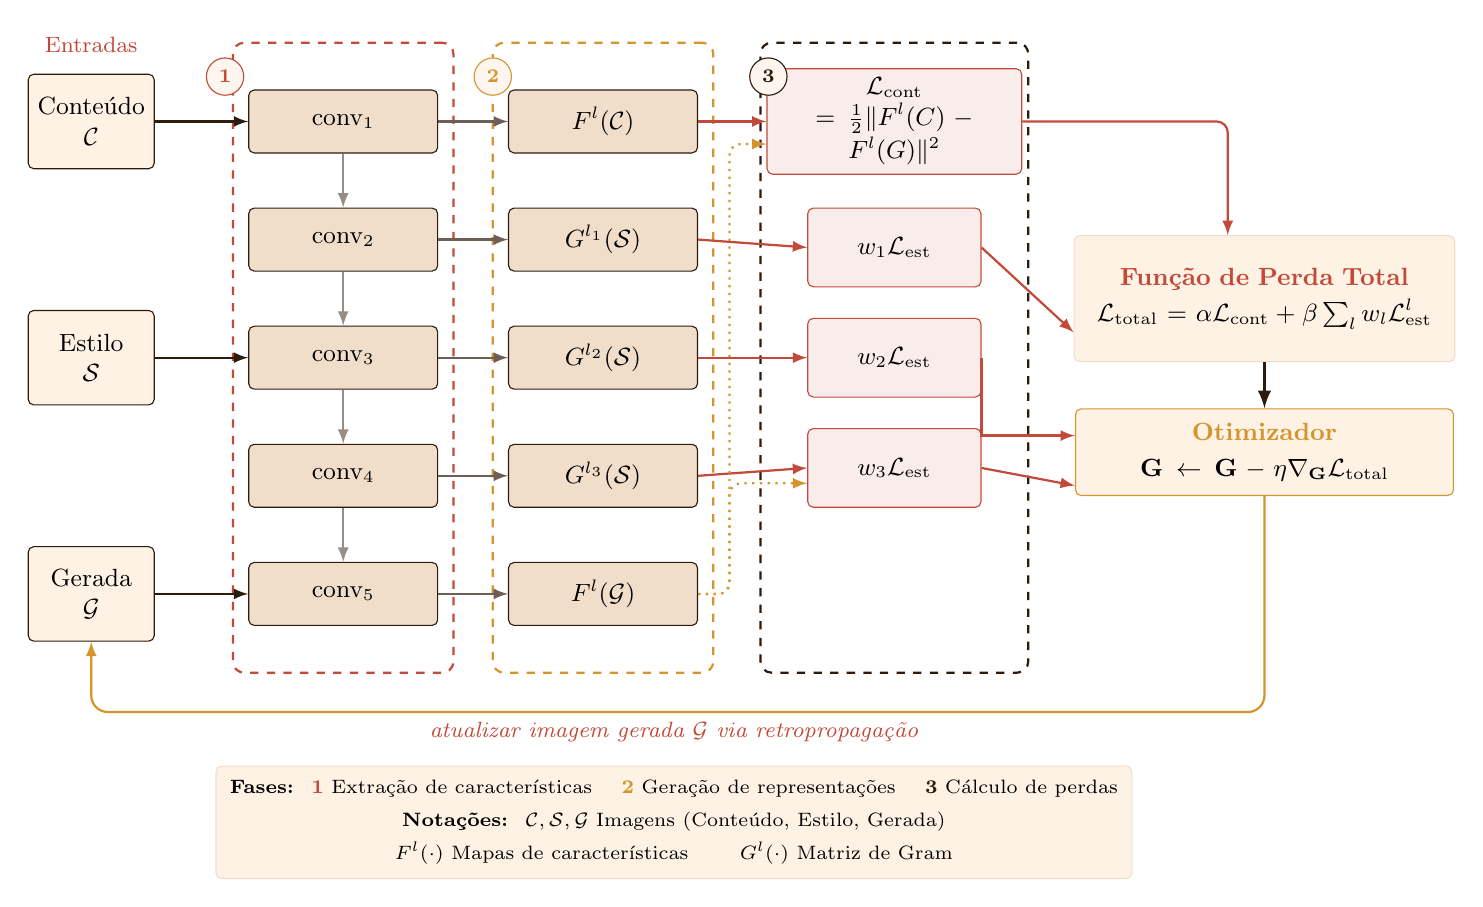
\begin{tikzpicture}[
    >=latex,
    box/.style={draw=wp-text, fill=wp-light, rounded corners=2pt, minimum width=2.4cm, minimum height=0.8cm, align=center, font=\small},
    img/.style={draw=wp-text, fill=wp-code, rounded corners=2pt, minimum width=1.6cm, minimum height=1.2cm, align=center, font=\small},
    loss/.style={draw=wp-primary, fill=wp-primary!10, rounded corners=2pt, minimum width=2.2cm, minimum height=1.0cm, align=center, font=\small},
    cnn/.style={draw=wp-primary, dashed, line width=0.8pt, fill=none, rounded corners=4pt, minimum width=2.8cm, minimum height=8cm, align=center, font=\small},
    grambox/.style={draw=wp-accent, dashed, line width=0.8pt, fill=none, rounded corners=4pt, minimum width=2.8cm, minimum height=8cm, align=center, font=\small},
    lossbox/.style={draw=wp-text, dashed, line width=0.8pt, fill=none, rounded corners=4pt, minimum width=3.4cm, minimum height=8cm, align=center, font=\small},
    conn/.style={->, draw=wp-primary, thick},
    label/.style={font=\footnotesize, text=wp-primary},
    tuftebox/.style={draw=wp-light, fill=wp-code, rounded corners=2pt, align=center}
]

% =========================================================================
% ENTRADAS: TENSORES DE IMAGEM SIMPLIFICADOS
% =========================================================================
\node[img] (content) at (0, 3.0)  {Conteúdo\\$\mathcal{C}$};
\node[img] (style)   at (0, 0.0)  {Estilo\\$\mathcal{S}$};
\node[img] (gen)     at (0, -3.0) {Gerada\\$\mathcal{G}$};

\node[label, above=4.2pt] at (content.north) {Entradas};

% =========================================================================
% CAMADAS DA CNN (Fase 1 - Container unificado)
% =========================================================================
\node[cnn] (cnn_box) at (3.2, 0) {};

\node[box] (conv1) at (3.2, 3.0)  {conv$_1$};
\node[box] (conv2) at (3.2, 1.5)  {conv$_2$};
\node[box] (conv3) at (3.2, 0.0)  {conv$_3$};
\node[box] (conv4) at (3.2, -1.5) {conv$_4$};
\node[box] (conv5) at (3.2, -3.0) {conv$_5$};

% Fluxo interno da CNN
\draw[->, draw=wp-text!50, thick] (conv1) -- (conv2);
\draw[->, draw=wp-text!50, thick] (conv2) -- (conv3);
\draw[->, draw=wp-text!50, thick] (conv3) -- (conv4);
\draw[->, draw=wp-text!50, thick] (conv4) -- (conv5);

% Conexões das entradas para a CNN
\draw[->, draw=wp-text, thick] (content.east) -- (conv1.west);
\draw[->, draw=wp-text, thick] (style.east)   -- (conv3.west);
\draw[->, draw=wp-text, thick] (gen.east)     -- (conv5.west);


% =========================================================================
% MAPAS DE CARACTERÍSTICAS E MATRIZES DE GRAM (Fase 2)
% =========================================================================
\node[grambox] (gram_container) at (6.5, 0) {};

\node[box] (fm_c)  at (6.5,  3.0) {$F^l(\mathcal{C})$};
\node[box] (gm_s1) at (6.5,  1.5) {$G^{l_1}(\mathcal{S})$};
\node[box] (gm_s2) at (6.5,  0.0) {$G^{l_2}(\mathcal{S})$};
\node[box] (gm_s3) at (6.5, -1.5) {$G^{l_3}(\mathcal{S})$};
\node[box] (fm_g)  at (6.5, -3.0) {$F^l(\mathcal{G})$};

\draw[->, draw=wp-text!70, thick] (conv1.east) -- (fm_c.west);
\draw[->, draw=wp-text!70, thick] (conv2.east) -- (gm_s1.west);
\draw[->, draw=wp-text!70, thick] (conv3.east) -- (gm_s2.west);
\draw[->, draw=wp-text!70, thick] (conv4.east) -- (gm_s3.west);
\draw[->, draw=wp-text!70, thick] (conv5.east) -- (fm_g.west);


% =========================================================================
% COMPUTAÇÃO DE PERDAS (Fase 3)
% =========================================================================
\node[lossbox] (loss_container) at (10.2, 0) {};

\node[loss, text width=3.0cm] (l_c) at (10.2, 3.0) {$\mathcal{L}_{\mathrm{cont}}$\\$=\frac{1}{2}\|F^l(C)-F^l(G)\|^2$};
\node[loss] (l_s1) at (10.2,  1.4) {$w_1\mathcal{L}_{\mathrm{est}}$};
\node[loss] (l_s2) at (10.2,  0.0) {$w_2\mathcal{L}_{\mathrm{est}}$};
\node[loss] (l_s3) at (10.2, -1.4) {$w_3\mathcal{L}_{\mathrm{est}}$};

\draw[conn] (fm_c.east)  -- (l_c.west);
\draw[conn] (gm_s1.east) -- (l_s1.west);
\draw[conn] (gm_s2.east) -- (l_s2.west);
\draw[conn] (gm_s3.east) -- (l_s3.west);

% Feedback do G para as perdas
\draw[->, draw=wp-accent, thick, dotted, rounded corners=4pt] (fm_g.east) -- ++(0.4,0) |- (l_c.190);
\draw[->, draw=wp-accent, thick, dotted, rounded corners=4pt] (fm_g.east) -- ++(0.4,0) |- (l_s3.190);


% =========================================================================
% FUNÇÃO DE PERDA TOTAL & OTIMIZADOR
% =========================================================================
\node[tuftebox, minimum width=4.8cm, minimum height=1.6cm, text width=4.6cm, font=\small] (l_total) at (14.9, 0.75) {
    \textbf{\color{wp-primary}Função de Perda Total}\\[2pt] 
    $\mathcal{L}_{\mathrm{total}} = \alpha\mathcal{L}_{\mathrm{cont}} + \beta\sum_l w_l\mathcal{L}_{\mathrm{est}}^l$
};

\node[draw=wp-accent, fill=wp-code, rounded corners=2pt, minimum width=4.8cm, minimum height=1.1cm, text width=4.2cm, font=\small, align=center] (opt) at (14.9, -1.2) {
    \textbf{\color{wp-accent}Otimizador}\\[2pt] 
    $\mathbf{G} \leftarrow \mathbf{G} - \eta\nabla_{\mathbf{G}}\mathcal{L}_{\mathrm{total}}$
};

% Conexões para a direita
\draw[->, draw=wp-primary, thick, rounded corners=4pt] (l_c.east) -| (l_total.120);
\draw[->, draw=wp-primary, thick] (l_s1.east) -- (l_total.190);
\draw[->, draw=wp-primary, thick] (l_s2.east) |- (opt.175);
\draw[->, draw=wp-primary, thick] (l_s3.east) -- (opt.190);

\draw[->, draw=wp-text, very thick] (l_total.south) -- (opt.north);


% =========================================================================
% FASES DE PROCESSAMENTO (Indicadores Numéricos)
% =========================================================================
\node[draw=wp-primary, fill=wp-bg, circle, inner sep=2.5pt, font=\scriptsize\bfseries, text=wp-primary] at (1.7, 3.57) {1};
\node[draw=wp-accent, fill=wp-bg, circle, inner sep=2.5pt, font=\scriptsize\bfseries, text=wp-accent] at (5.1, 3.57) {2};
\node[draw=wp-text, fill=wp-bg, circle, inner sep=2.5pt, font=\scriptsize\bfseries, text=wp-text] at (8.6, 3.57) {3};


% =========================================================================
% FEEDBACK LOOP (Passando horizontalmente por baixo)
% =========================================================================
\draw[->, draw=wp-accent, thick, rounded corners=6pt] 
    (opt.south) -- (14.9, -4.5) -- (0, -4.5) -- (gen.south);

\node[label, font=\itshape\footnotesize, anchor=north] at (7.4, -4.5) 
    {atualizar imagem gerada $\mathcal{G}$ via retropropagação};


% =========================================================================
% LEGENDA DAS FASES E NOTAÇÕES REPOSICIONADA
% =========================================================================
\node[tuftebox, minimum width=10.0cm, minimum height=1.0cm, inner sep=5pt] (legenda) at (7.4, -5.9) {
    \scriptsize 
    \textbf{Fases:} \ 
    \textbf{\color{wp-primary}1} Extração de características \quad 
    \textbf{\color{wp-accent}2} Geração de representações \quad 
    \textbf{\color{wp-text}3} Cálculo de perdas \\
    \scriptsize
    \textbf{Notações:} \ 
    $\mathcal{C}, \mathcal{S}, \mathcal{G}$ Imagens (Conteúdo, Estilo, Gerada)\\
    \scriptsize
    $F^l(\cdot)$ Mapas de características \qquad 
    $G^l(\cdot)$ Matriz de Gram
};

\end{tikzpicture}
}
\caption{Pipeline completo de Style Transfer. Três imagens ($\mathcal{C}$, $\mathcal{S}$, $\mathcal{G}$) passam por uma CNN pré-treinada. Mapas de características de $\mathcal{C}$ e $\mathcal{G}$ em uma camada profunda definem a perda de conteúdo. Matrizes de Gram de $\mathcal{S}$ e $\mathcal{G}$ em múltiplos níveis definem a perda de estilo. A perda total é minimizada via gradiente descendente, atualizando $\mathcal{G}$.}
\label{fig:style-transfer-pipeline}
\end{figure*}
\begin{figure*}[htbp]
\centering
\resizebox{\textwidth}{!}{%
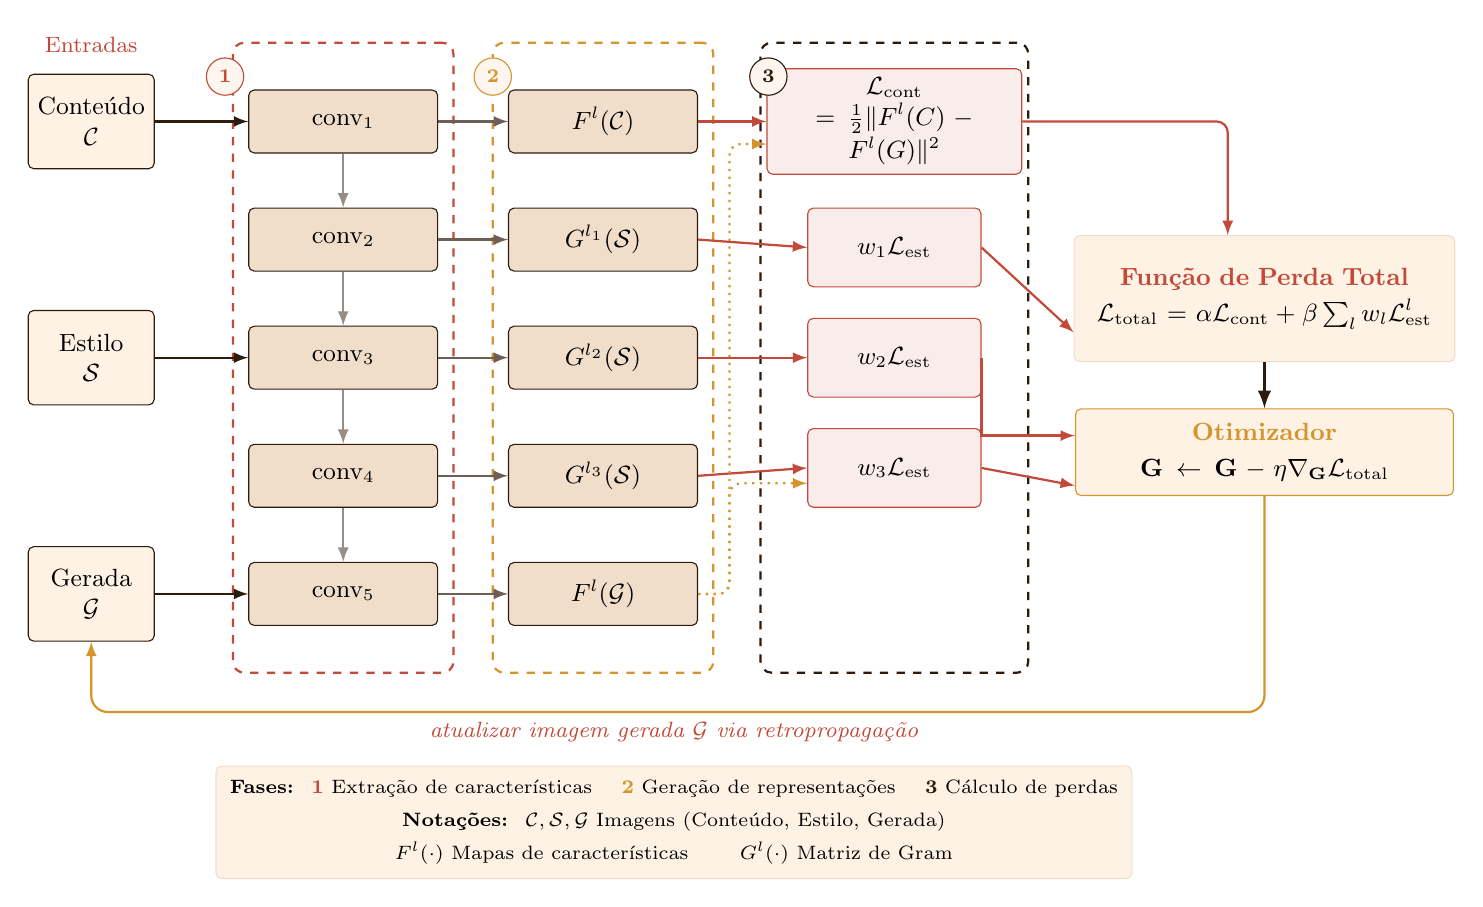
\begin{tikzpicture}[
    >=latex,
    box/.style={draw=wp-text, fill=wp-light, rounded corners=2pt, minimum width=2.4cm, minimum height=0.8cm, align=center, font=\small},
    img/.style={draw=wp-text, fill=wp-code, rounded corners=2pt, minimum width=1.6cm, minimum height=1.2cm, align=center, font=\small},
    loss/.style={draw=wp-primary, fill=wp-primary!10, rounded corners=2pt, minimum width=2.2cm, minimum height=1.0cm, align=center, font=\small},
    cnn/.style={draw=wp-primary, dashed, line width=0.8pt, fill=none, rounded corners=4pt, minimum width=2.8cm, minimum height=8cm, align=center, font=\small},
    grambox/.style={draw=wp-accent, dashed, line width=0.8pt, fill=none, rounded corners=4pt, minimum width=2.8cm, minimum height=8cm, align=center, font=\small},
    lossbox/.style={draw=wp-text, dashed, line width=0.8pt, fill=none, rounded corners=4pt, minimum width=3.4cm, minimum height=8cm, align=center, font=\small},
    conn/.style={->, draw=wp-primary, thick},
    label/.style={font=\footnotesize, text=wp-primary},
    tuftebox/.style={draw=wp-light, fill=wp-code, rounded corners=2pt, align=center}
]

% =========================================================================
% ENTRADAS: TENSORES DE IMAGEM SIMPLIFICADOS
% =========================================================================
\node[img] (content) at (0, 3.0)  {Conteúdo\\$\mathcal{C}$};
\node[img] (style)   at (0, 0.0)  {Estilo\\$\mathcal{S}$};
\node[img] (gen)     at (0, -3.0) {Gerada\\$\mathcal{G}$};

\node[label, above=4.2pt] at (content.north) {Entradas};

% =========================================================================
% CAMADAS DA CNN (Fase 1 - Container unificado)
% =========================================================================
\node[cnn] (cnn_box) at (3.2, 0) {};

\node[box] (conv1) at (3.2, 3.0)  {conv$_1$};
\node[box] (conv2) at (3.2, 1.5)  {conv$_2$};
\node[box] (conv3) at (3.2, 0.0)  {conv$_3$};
\node[box] (conv4) at (3.2, -1.5) {conv$_4$};
\node[box] (conv5) at (3.2, -3.0) {conv$_5$};

% Fluxo interno da CNN
\draw[->, draw=wp-text!50, thick] (conv1) -- (conv2);
\draw[->, draw=wp-text!50, thick] (conv2) -- (conv3);
\draw[->, draw=wp-text!50, thick] (conv3) -- (conv4);
\draw[->, draw=wp-text!50, thick] (conv4) -- (conv5);

% Conexões das entradas para a CNN
\draw[->, draw=wp-text, thick] (content.east) -- (conv1.west);
\draw[->, draw=wp-text, thick] (style.east)   -- (conv3.west);
\draw[->, draw=wp-text, thick] (gen.east)     -- (conv5.west);


% =========================================================================
% MAPAS DE CARACTERÍSTICAS E MATRIZES DE GRAM (Fase 2)
% =========================================================================
\node[grambox] (gram_container) at (6.5, 0) {};

\node[box] (fm_c)  at (6.5,  3.0) {$F^l(\mathcal{C})$};
\node[box] (gm_s1) at (6.5,  1.5) {$G^{l_1}(\mathcal{S})$};
\node[box] (gm_s2) at (6.5,  0.0) {$G^{l_2}(\mathcal{S})$};
\node[box] (gm_s3) at (6.5, -1.5) {$G^{l_3}(\mathcal{S})$};
\node[box] (fm_g)  at (6.5, -3.0) {$F^l(\mathcal{G})$};

\draw[->, draw=wp-text!70, thick] (conv1.east) -- (fm_c.west);
\draw[->, draw=wp-text!70, thick] (conv2.east) -- (gm_s1.west);
\draw[->, draw=wp-text!70, thick] (conv3.east) -- (gm_s2.west);
\draw[->, draw=wp-text!70, thick] (conv4.east) -- (gm_s3.west);
\draw[->, draw=wp-text!70, thick] (conv5.east) -- (fm_g.west);


% =========================================================================
% COMPUTAÇÃO DE PERDAS (Fase 3)
% =========================================================================
\node[lossbox] (loss_container) at (10.2, 0) {};

\node[loss, text width=3.0cm] (l_c) at (10.2, 3.0) {$\mathcal{L}_{\mathrm{cont}}$\\$=\frac{1}{2}\|F^l(C)-F^l(G)\|^2$};
\node[loss] (l_s1) at (10.2,  1.4) {$w_1\mathcal{L}_{\mathrm{est}}$};
\node[loss] (l_s2) at (10.2,  0.0) {$w_2\mathcal{L}_{\mathrm{est}}$};
\node[loss] (l_s3) at (10.2, -1.4) {$w_3\mathcal{L}_{\mathrm{est}}$};

\draw[conn] (fm_c.east)  -- (l_c.west);
\draw[conn] (gm_s1.east) -- (l_s1.west);
\draw[conn] (gm_s2.east) -- (l_s2.west);
\draw[conn] (gm_s3.east) -- (l_s3.west);

% Feedback do G para as perdas
\draw[->, draw=wp-accent, thick, dotted, rounded corners=4pt] (fm_g.east) -- ++(0.4,0) |- (l_c.190);
\draw[->, draw=wp-accent, thick, dotted, rounded corners=4pt] (fm_g.east) -- ++(0.4,0) |- (l_s3.190);


% =========================================================================
% FUNÇÃO DE PERDA TOTAL & OTIMIZADOR
% =========================================================================
\node[tuftebox, minimum width=4.8cm, minimum height=1.6cm, text width=4.6cm, font=\small] (l_total) at (14.9, 0.75) {
    \textbf{\color{wp-primary}Função de Perda Total}\\[2pt] 
    $\mathcal{L}_{\mathrm{total}} = \alpha\mathcal{L}_{\mathrm{cont}} + \beta\sum_l w_l\mathcal{L}_{\mathrm{est}}^l$
};

\node[draw=wp-accent, fill=wp-code, rounded corners=2pt, minimum width=4.8cm, minimum height=1.1cm, text width=4.2cm, font=\small, align=center] (opt) at (14.9, -1.2) {
    \textbf{\color{wp-accent}Otimizador}\\[2pt] 
    $\mathbf{G} \leftarrow \mathbf{G} - \eta\nabla_{\mathbf{G}}\mathcal{L}_{\mathrm{total}}$
};

% Conexões para a direita
\draw[->, draw=wp-primary, thick, rounded corners=4pt] (l_c.east) -| (l_total.120);
\draw[->, draw=wp-primary, thick] (l_s1.east) -- (l_total.190);
\draw[->, draw=wp-primary, thick] (l_s2.east) |- (opt.175);
\draw[->, draw=wp-primary, thick] (l_s3.east) -- (opt.190);

\draw[->, draw=wp-text, very thick] (l_total.south) -- (opt.north);


% =========================================================================
% FASES DE PROCESSAMENTO (Indicadores Numéricos)
% =========================================================================
\node[draw=wp-primary, fill=wp-bg, circle, inner sep=2.5pt, font=\scriptsize\bfseries, text=wp-primary] at (1.7, 3.57) {1};
\node[draw=wp-accent, fill=wp-bg, circle, inner sep=2.5pt, font=\scriptsize\bfseries, text=wp-accent] at (5.1, 3.57) {2};
\node[draw=wp-text, fill=wp-bg, circle, inner sep=2.5pt, font=\scriptsize\bfseries, text=wp-text] at (8.6, 3.57) {3};


% =========================================================================
% FEEDBACK LOOP (Passando horizontalmente por baixo)
% =========================================================================
\draw[->, draw=wp-accent, thick, rounded corners=6pt] 
    (opt.south) -- (14.9, -4.5) -- (0, -4.5) -- (gen.south);

\node[label, font=\itshape\footnotesize, anchor=north] at (7.4, -4.5) 
    {atualizar imagem gerada $\mathcal{G}$ via retropropagação};


% =========================================================================
% LEGENDA DAS FASES E NOTAÇÕES REPOSICIONADA
% =========================================================================
\node[tuftebox, minimum width=10.0cm, minimum height=1.0cm, inner sep=5pt] (legenda) at (7.4, -5.9) {
    \scriptsize 
    \textbf{Fases:} \ 
    \textbf{\color{wp-primary}1} Extração de características \quad 
    \textbf{\color{wp-accent}2} Geração de representações \quad 
    \textbf{\color{wp-text}3} Cálculo de perdas \\
    \scriptsize
    \textbf{Notações:} \ 
    $\mathcal{C}, \mathcal{S}, \mathcal{G}$ Imagens (Conteúdo, Estilo, Gerada)\\
    \scriptsize
    $F^l(\cdot)$ Mapas de características \qquad 
    $G^l(\cdot)$ Matriz de Gram
};

\end{tikzpicture}
}
\caption{Pipeline completo de Style Transfer. Três imagens ($\mathcal{C}$, $\mathcal{S}$, $\mathcal{G}$) passam por uma CNN pré-treinada. Mapas de características de $\mathcal{C}$ e $\mathcal{G}$ em uma camada profunda definem a perda de conteúdo. Matrizes de Gram de $\mathcal{S}$ e $\mathcal{G}$ em múltiplos níveis definem a perda de estilo. A perda total é minimizada via gradiente descendente, atualizando $\mathcal{G}$.}
\label{fig:style-transfer-pipeline}
\end{figure*}

\subsection{Representação do Conteúdo}

O conteúdo de uma imagem está associado às características de alto nível, como formas e objetos, que são capturados principalmente pelas camadas mais profundas da CNN. Para representar o conteúdo, utilizamos os mapas de características $F^l(C)$ e $F^l(G)$ extraídos de uma camada específica $l$ da rede.

A função de perda do conteúdo mede a diferença entre as representações da imagem de conteúdo e da imagem gerada na camada $l$. Essa diferença é calculada como o erro quadrático médio entre os mapas de características:

\begin{equation*}
    \mathcal{L}_{\text{conteúdo}} (C, G, l) = \frac{1}{2} \sum_{i,j} \left(F_{ij}^l(G) - F_{ij}^l(C)\right)^2
\end{equation*}

Onde:
- $F_{ij}^l(C)$ é o valor do mapa de características da imagem de conteúdo na posição $(i,j)$ da camada $l$.
- $F_{ij}^l(G)$ é o valor correspondente na imagem gerada.

\subsection{Representação do Estilo}

O estilo de uma imagem está associado às características de baixo e médio nível, como texturas, cores e padrões, que são capturados pelas correlações entre os mapas de características em \textbf{múltiplas camadas} $L$ da CNN. Para representar o estilo, utilizamos a matriz de Gram $G^l$, que mede as correlações entre os mapas de características na camada $l$.

A função de perda do estilo é definida como a soma ponderada das diferenças entre as matrizes de Gram da imagem de estilo e da imagem gerada em várias camadas:

\begin{equation*}
    \mathcal{L}_{\text{estilo}} (S, G, L) = \sum_{l \in L} w_l \cdot \frac{1}{4N_l^2 M_l^2} \sum_{i,j} \left(G^l_{ij}(G) - G^l_{ij}(S)\right)^2
\end{equation*}

Onde:
- $w_l$ é o peso associado à camada $l$, que controla sua contribuição para a perda total.
- $N_l$ é o número de mapas de características na camada $l$.
- $M_l$ é o tamanho espacial (altura $\times$ largura) dos mapas de características na camada $l$.
- $G^l_{ij}(S)$ e $G^l_{ij}(G)$ são os elementos das matrizes de Gram para a imagem de estilo e a imagem gerada, respectivamente.

\subsection{Otimização}

A imagem gerada $G$ é obtida minimizando uma função de perda total, que combina as perdas de conteúdo e estilo:

\begin{equation*}
    \mathcal{L}_{\text{total}} (C, S, G) = \alpha \cdot \mathcal{L}_{\text{conteúdo}} (C, G, l) + \beta \cdot \mathcal{L}_{\text{estilo}} (S, G, L)
\end{equation*}

Onde $\alpha$ e $\beta$ são hiperparâmetros que controlam o equilíbrio entre a preservação do conteúdo e a transferência do estilo.

Por meio de técnicas de otimização, como o gradiente descendente, a imagem gerada é iterativamente ajustada até que a perda total seja minimizada, resultando em uma imagem que combina o conteúdo de $C$ com o estilo de $S$.


O objetivo é minimizar \( \mathcal{L}_{\text{total}} \) em relação à imagem gerada \( \mathbf{G} \). Isso é feito usando Gradient Descent:
\[
\mathbf{G} \leftarrow \mathbf{G} - \eta \cdot \nabla_{\mathbf{G}} \mathcal{L}_{\text{total}}
\]
Onde \( \eta \) é a taxa de aprendizado.

% Style Transfer — Loop de Otimização (Layout em Carrossel Horário)
% Uso: % Style Transfer — Loop de Otimização (Layout em Carrossel Horário)
% Uso: % Style Transfer — Loop de Otimização (Layout em Carrossel Horário)
% Uso: \input{resources/style-transfer/optimization-loop.tex}
\begin{figure*}[htbp]
\centering
\resizebox{\textwidth}{!}{%
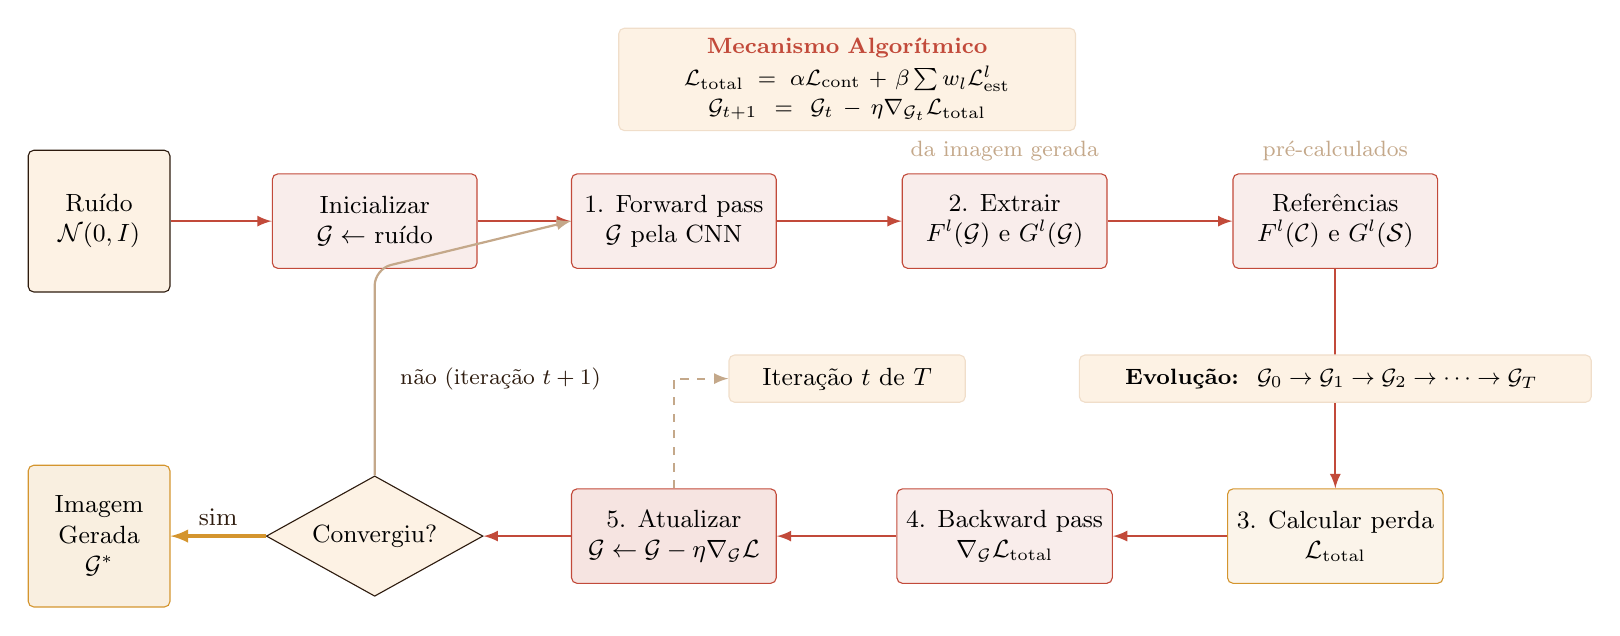
\begin{tikzpicture}[
    >=latex,
    box/.style={draw=wp-text, fill=wp-light, rounded corners=2pt, minimum width=2.5cm, minimum height=1.0cm, align=center, font=\small},
    proc/.style={draw=wp-primary, fill=wp-primary!10, rounded corners=2pt, minimum width=2.6cm, minimum height=1.2cm, align=center, font=\small},
    img/.style={draw=wp-text, fill=wp-code, rounded corners=2pt, minimum width=1.8cm, minimum height=1.8cm, align=center, font=\small},
    conn/.style={->, draw=wp-primary, thick},
    label/.style={font=\footnotesize, text=wp-muted},
    tuftebox/.style={draw=wp-light, fill=wp-code, rounded corners=2pt, align=center}
]

% =========================================================================
% ESTÁGIO 1: INICIALIZAÇÃO EXTERNA (Fora do loop principal)
% =========================================================================
\node[img] (start) at (-3.5, 3.0) {Ruído\\$\mathcal{N}(0,I)$};
\node[proc] (init) at (0, 3.0) {Inicializar\\$\mathcal{G} \leftarrow$ ruído};

\draw[conn] (start) -- (init);

% =========================================================================
% ESTÁGIO 2: FLUXO SUPERIOR (Esquerda para a Direita)
% =========================================================================
\node[proc] (forward) at (3.8, 3.0) {1. Forward pass\\$\mathcal{G}$ pela CNN};
\node[proc] (features) at (8.0, 3.0) {2. Extrair\\$F^l(\mathcal{G})$ e $G^l(\mathcal{G})$};
\node[proc] (targets)  at (12.2, 3.0) {Referências\\$F^l(\mathcal{C})$ e $G^l(\mathcal{S})$};

\draw[conn] (init) -- (forward);
\draw[conn] (forward) -- (features);
\draw[conn] (features) -- (targets);

\node[label, above=1pt] at (features.north) {da imagem gerada};
\node[label, above=1pt] at (targets.north) {pré-calculados};


% =========================================================================
% ESTÁGIO 3: DESCIDA E RETORNO INFERIOR (Direita para a Esquerda)
% =========================================================================
\node[proc, fill=wp-accent!10, draw=wp-accent] (loss) at (12.2, -1.0) {3. Calcular perda\\$\mathcal{L}_{\mathrm{total}}$};
\node[proc] (backward) at (8.0, -1.0) {4. Backward pass\\$\nabla_{\mathcal{G}} \mathcal{L}_{\mathrm{total}}$};
\node[proc, fill=wp-primary!15, draw=wp-primary] (update) at (3.8, -1.0) {5. Atualizar\\$\mathcal{G} \leftarrow \mathcal{G} - \eta \nabla_{\mathcal{G}} \mathcal{L}$};

% Descida vertical na extrema direita
\draw[conn] (targets.south) -- (loss.north);

% Fluxo de retorno para a esquerda na base
\draw[conn] (loss) -- (backward);
\draw[conn] (backward) -- (update);


% =========================================================================
% ESTÁGIO 4: CIRCUITO DE RETORNO DO LOOP (Fechamento à Esquerda)
% =========================================================================
\node[draw=wp-text, diamond, fill=wp-code, aspect=1.8, minimum width=2.0cm, font=\small] (decide) at (0, -1.0) {Convergiu?};
\node[img, fill=wp-accent!15, draw=wp-accent] (output) at (-3.5, -1.0) {Imagem\\Gerada\\$\mathcal{G}^*$};

\draw[conn] (update) -- (decide);
\draw[->, draw=wp-accent, very thick] (decide) -- node[above, font=\small, text=wp-text] {sim} (output);

% O FECHAMENTO DO ANEL: "Não" sobe em linha reta vertical direto para o Forward Pass
\draw[->, draw=wp-muted, thick, rounded corners=6pt] (decide.north) -- (init.south) -- (forward.west);
\node[text=wp-text, font=\footnotesize, anchor=west] at (0.2, 1.0) {não (iteração $t+1$)};


% =========================================================================
% CAIXAS DE CONTEXTO E METADADOS METODOLÓGICOS (Zonas Vazias Limpas)
% =========================================================================
% Central inferior
\node[draw=wp-light, fill=wp-code, rounded corners=2pt, minimum width=3.0cm, minimum height=0.6cm, font=\small] (iter) at (6.0, 1.0) {Iteração $t$ de $T$};
\draw[->, draw=wp-muted, thick, dashed] (update.north) |- (iter.west);

\node[tuftebox, minimum width=6.5cm, minimum height=0.6cm, inner sep=4pt] at (12.2, 1.0) {
    \footnotesize \textbf{Evolução:} \ $\mathcal{G}_0 \rightarrow \mathcal{G}_1 \rightarrow \mathcal{G}_2 \rightarrow \cdots \rightarrow \mathcal{G}_T$
};

% Bloco de fórmulas suspenso no centro-topo sem atrapalhar setas
\node[tuftebox, minimum width=5.8cm, minimum height=1.3cm, text width=5.5cm, font=\footnotesize] at (6.0, 4.8) {
    \textbf{\color{wp-primary}Mecanismo Algorítmico}\\[2pt]
    $\mathcal{L}_{\mathrm{total}} = \alpha\mathcal{L}_{\mathrm{cont}} + \beta\sum w_l\mathcal{L}_{\mathrm{est}}^l$ \\[1pt]
    $\mathbf{\mathcal{G}}_{t+1} = \mathbf{\mathcal{G}}_t - \eta \nabla_{\mathbf{\mathcal{G}}_t}\mathcal{L}_{\mathrm{total}}$
};

\end{tikzpicture}
}
\caption{Loop de otimização iterativo do Style Transfer organizado em anel de fluxo horário.}
\label{fig:optimization-loop}
\end{figure*}
\begin{figure*}[htbp]
\centering
\resizebox{\textwidth}{!}{%
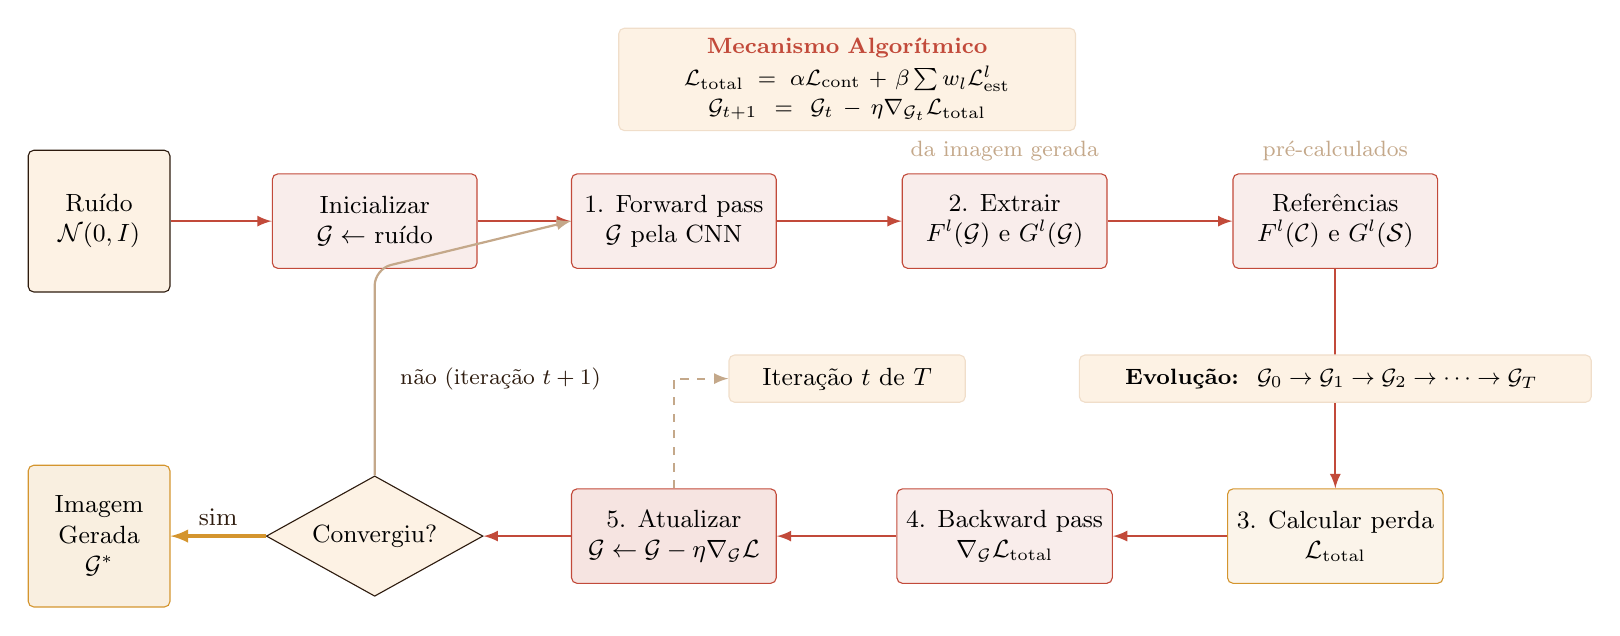
\begin{tikzpicture}[
    >=latex,
    box/.style={draw=wp-text, fill=wp-light, rounded corners=2pt, minimum width=2.5cm, minimum height=1.0cm, align=center, font=\small},
    proc/.style={draw=wp-primary, fill=wp-primary!10, rounded corners=2pt, minimum width=2.6cm, minimum height=1.2cm, align=center, font=\small},
    img/.style={draw=wp-text, fill=wp-code, rounded corners=2pt, minimum width=1.8cm, minimum height=1.8cm, align=center, font=\small},
    conn/.style={->, draw=wp-primary, thick},
    label/.style={font=\footnotesize, text=wp-muted},
    tuftebox/.style={draw=wp-light, fill=wp-code, rounded corners=2pt, align=center}
]

% =========================================================================
% ESTÁGIO 1: INICIALIZAÇÃO EXTERNA (Fora do loop principal)
% =========================================================================
\node[img] (start) at (-3.5, 3.0) {Ruído\\$\mathcal{N}(0,I)$};
\node[proc] (init) at (0, 3.0) {Inicializar\\$\mathcal{G} \leftarrow$ ruído};

\draw[conn] (start) -- (init);

% =========================================================================
% ESTÁGIO 2: FLUXO SUPERIOR (Esquerda para a Direita)
% =========================================================================
\node[proc] (forward) at (3.8, 3.0) {1. Forward pass\\$\mathcal{G}$ pela CNN};
\node[proc] (features) at (8.0, 3.0) {2. Extrair\\$F^l(\mathcal{G})$ e $G^l(\mathcal{G})$};
\node[proc] (targets)  at (12.2, 3.0) {Referências\\$F^l(\mathcal{C})$ e $G^l(\mathcal{S})$};

\draw[conn] (init) -- (forward);
\draw[conn] (forward) -- (features);
\draw[conn] (features) -- (targets);

\node[label, above=1pt] at (features.north) {da imagem gerada};
\node[label, above=1pt] at (targets.north) {pré-calculados};


% =========================================================================
% ESTÁGIO 3: DESCIDA E RETORNO INFERIOR (Direita para a Esquerda)
% =========================================================================
\node[proc, fill=wp-accent!10, draw=wp-accent] (loss) at (12.2, -1.0) {3. Calcular perda\\$\mathcal{L}_{\mathrm{total}}$};
\node[proc] (backward) at (8.0, -1.0) {4. Backward pass\\$\nabla_{\mathcal{G}} \mathcal{L}_{\mathrm{total}}$};
\node[proc, fill=wp-primary!15, draw=wp-primary] (update) at (3.8, -1.0) {5. Atualizar\\$\mathcal{G} \leftarrow \mathcal{G} - \eta \nabla_{\mathcal{G}} \mathcal{L}$};

% Descida vertical na extrema direita
\draw[conn] (targets.south) -- (loss.north);

% Fluxo de retorno para a esquerda na base
\draw[conn] (loss) -- (backward);
\draw[conn] (backward) -- (update);


% =========================================================================
% ESTÁGIO 4: CIRCUITO DE RETORNO DO LOOP (Fechamento à Esquerda)
% =========================================================================
\node[draw=wp-text, diamond, fill=wp-code, aspect=1.8, minimum width=2.0cm, font=\small] (decide) at (0, -1.0) {Convergiu?};
\node[img, fill=wp-accent!15, draw=wp-accent] (output) at (-3.5, -1.0) {Imagem\\Gerada\\$\mathcal{G}^*$};

\draw[conn] (update) -- (decide);
\draw[->, draw=wp-accent, very thick] (decide) -- node[above, font=\small, text=wp-text] {sim} (output);

% O FECHAMENTO DO ANEL: "Não" sobe em linha reta vertical direto para o Forward Pass
\draw[->, draw=wp-muted, thick, rounded corners=6pt] (decide.north) -- (init.south) -- (forward.west);
\node[text=wp-text, font=\footnotesize, anchor=west] at (0.2, 1.0) {não (iteração $t+1$)};


% =========================================================================
% CAIXAS DE CONTEXTO E METADADOS METODOLÓGICOS (Zonas Vazias Limpas)
% =========================================================================
% Central inferior
\node[draw=wp-light, fill=wp-code, rounded corners=2pt, minimum width=3.0cm, minimum height=0.6cm, font=\small] (iter) at (6.0, 1.0) {Iteração $t$ de $T$};
\draw[->, draw=wp-muted, thick, dashed] (update.north) |- (iter.west);

\node[tuftebox, minimum width=6.5cm, minimum height=0.6cm, inner sep=4pt] at (12.2, 1.0) {
    \footnotesize \textbf{Evolução:} \ $\mathcal{G}_0 \rightarrow \mathcal{G}_1 \rightarrow \mathcal{G}_2 \rightarrow \cdots \rightarrow \mathcal{G}_T$
};

% Bloco de fórmulas suspenso no centro-topo sem atrapalhar setas
\node[tuftebox, minimum width=5.8cm, minimum height=1.3cm, text width=5.5cm, font=\footnotesize] at (6.0, 4.8) {
    \textbf{\color{wp-primary}Mecanismo Algorítmico}\\[2pt]
    $\mathcal{L}_{\mathrm{total}} = \alpha\mathcal{L}_{\mathrm{cont}} + \beta\sum w_l\mathcal{L}_{\mathrm{est}}^l$ \\[1pt]
    $\mathbf{\mathcal{G}}_{t+1} = \mathbf{\mathcal{G}}_t - \eta \nabla_{\mathbf{\mathcal{G}}_t}\mathcal{L}_{\mathrm{total}}$
};

\end{tikzpicture}
}
\caption{Loop de otimização iterativo do Style Transfer organizado em anel de fluxo horário.}
\label{fig:optimization-loop}
\end{figure*}
\begin{figure*}[htbp]
\centering
\resizebox{\textwidth}{!}{%
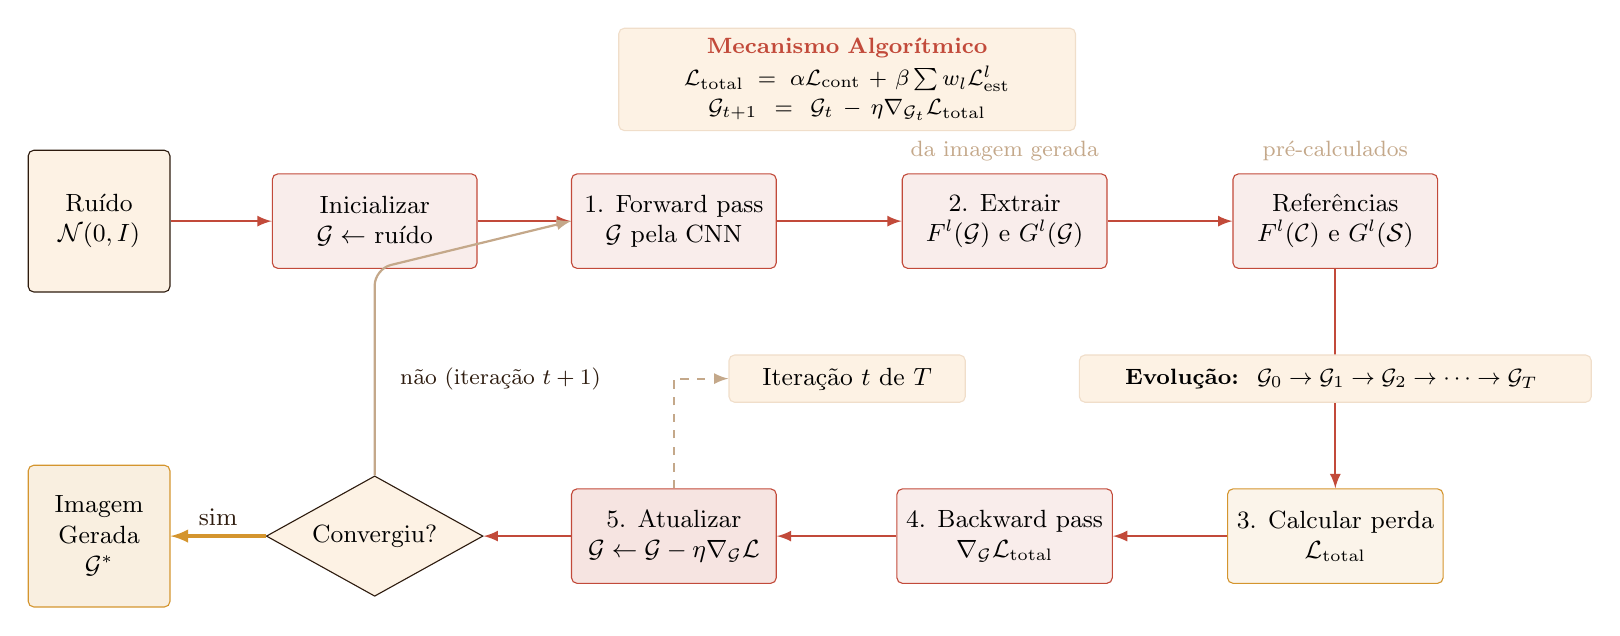
\begin{tikzpicture}[
    >=latex,
    box/.style={draw=wp-text, fill=wp-light, rounded corners=2pt, minimum width=2.5cm, minimum height=1.0cm, align=center, font=\small},
    proc/.style={draw=wp-primary, fill=wp-primary!10, rounded corners=2pt, minimum width=2.6cm, minimum height=1.2cm, align=center, font=\small},
    img/.style={draw=wp-text, fill=wp-code, rounded corners=2pt, minimum width=1.8cm, minimum height=1.8cm, align=center, font=\small},
    conn/.style={->, draw=wp-primary, thick},
    label/.style={font=\footnotesize, text=wp-muted},
    tuftebox/.style={draw=wp-light, fill=wp-code, rounded corners=2pt, align=center}
]

% =========================================================================
% ESTÁGIO 1: INICIALIZAÇÃO EXTERNA (Fora do loop principal)
% =========================================================================
\node[img] (start) at (-3.5, 3.0) {Ruído\\$\mathcal{N}(0,I)$};
\node[proc] (init) at (0, 3.0) {Inicializar\\$\mathcal{G} \leftarrow$ ruído};

\draw[conn] (start) -- (init);

% =========================================================================
% ESTÁGIO 2: FLUXO SUPERIOR (Esquerda para a Direita)
% =========================================================================
\node[proc] (forward) at (3.8, 3.0) {1. Forward pass\\$\mathcal{G}$ pela CNN};
\node[proc] (features) at (8.0, 3.0) {2. Extrair\\$F^l(\mathcal{G})$ e $G^l(\mathcal{G})$};
\node[proc] (targets)  at (12.2, 3.0) {Referências\\$F^l(\mathcal{C})$ e $G^l(\mathcal{S})$};

\draw[conn] (init) -- (forward);
\draw[conn] (forward) -- (features);
\draw[conn] (features) -- (targets);

\node[label, above=1pt] at (features.north) {da imagem gerada};
\node[label, above=1pt] at (targets.north) {pré-calculados};


% =========================================================================
% ESTÁGIO 3: DESCIDA E RETORNO INFERIOR (Direita para a Esquerda)
% =========================================================================
\node[proc, fill=wp-accent!10, draw=wp-accent] (loss) at (12.2, -1.0) {3. Calcular perda\\$\mathcal{L}_{\mathrm{total}}$};
\node[proc] (backward) at (8.0, -1.0) {4. Backward pass\\$\nabla_{\mathcal{G}} \mathcal{L}_{\mathrm{total}}$};
\node[proc, fill=wp-primary!15, draw=wp-primary] (update) at (3.8, -1.0) {5. Atualizar\\$\mathcal{G} \leftarrow \mathcal{G} - \eta \nabla_{\mathcal{G}} \mathcal{L}$};

% Descida vertical na extrema direita
\draw[conn] (targets.south) -- (loss.north);

% Fluxo de retorno para a esquerda na base
\draw[conn] (loss) -- (backward);
\draw[conn] (backward) -- (update);


% =========================================================================
% ESTÁGIO 4: CIRCUITO DE RETORNO DO LOOP (Fechamento à Esquerda)
% =========================================================================
\node[draw=wp-text, diamond, fill=wp-code, aspect=1.8, minimum width=2.0cm, font=\small] (decide) at (0, -1.0) {Convergiu?};
\node[img, fill=wp-accent!15, draw=wp-accent] (output) at (-3.5, -1.0) {Imagem\\Gerada\\$\mathcal{G}^*$};

\draw[conn] (update) -- (decide);
\draw[->, draw=wp-accent, very thick] (decide) -- node[above, font=\small, text=wp-text] {sim} (output);

% O FECHAMENTO DO ANEL: "Não" sobe em linha reta vertical direto para o Forward Pass
\draw[->, draw=wp-muted, thick, rounded corners=6pt] (decide.north) -- (init.south) -- (forward.west);
\node[text=wp-text, font=\footnotesize, anchor=west] at (0.2, 1.0) {não (iteração $t+1$)};


% =========================================================================
% CAIXAS DE CONTEXTO E METADADOS METODOLÓGICOS (Zonas Vazias Limpas)
% =========================================================================
% Central inferior
\node[draw=wp-light, fill=wp-code, rounded corners=2pt, minimum width=3.0cm, minimum height=0.6cm, font=\small] (iter) at (6.0, 1.0) {Iteração $t$ de $T$};
\draw[->, draw=wp-muted, thick, dashed] (update.north) |- (iter.west);

\node[tuftebox, minimum width=6.5cm, minimum height=0.6cm, inner sep=4pt] at (12.2, 1.0) {
    \footnotesize \textbf{Evolução:} \ $\mathcal{G}_0 \rightarrow \mathcal{G}_1 \rightarrow \mathcal{G}_2 \rightarrow \cdots \rightarrow \mathcal{G}_T$
};

% Bloco de fórmulas suspenso no centro-topo sem atrapalhar setas
\node[tuftebox, minimum width=5.8cm, minimum height=1.3cm, text width=5.5cm, font=\footnotesize] at (6.0, 4.8) {
    \textbf{\color{wp-primary}Mecanismo Algorítmico}\\[2pt]
    $\mathcal{L}_{\mathrm{total}} = \alpha\mathcal{L}_{\mathrm{cont}} + \beta\sum w_l\mathcal{L}_{\mathrm{est}}^l$ \\[1pt]
    $\mathbf{\mathcal{G}}_{t+1} = \mathbf{\mathcal{G}}_t - \eta \nabla_{\mathbf{\mathcal{G}}_t}\mathcal{L}_{\mathrm{total}}$
};

\end{tikzpicture}
}
\caption{Loop de otimização iterativo do Style Transfer organizado em anel de fluxo horário.}
\label{fig:optimization-loop}
\end{figure*}

\section{Autoencoders}

Autoencoders (AEs) são uma técnica de aprendizado não supervisionado que visa aprender representações compactas e eficientes de dados sem a necessidade de rótulos. Eles consistem em duas redes neurais principais: o \textbf{encoder} (codificador) e o \textbf{decoder} (decodificador). O encoder transforma os dados de entrada em uma representação codificada, enquanto o decoder tenta reconstruir os dados originais a partir dessa representação. Matematicamente, um autoencoder pode ser definido como:

\begin{equation*}
    E_{\phi}: \mathcal{X} \rightarrow \mathcal{Z} \quad \text{e} \quad D_{\theta}: \mathcal{Z} \rightarrow \mathcal{X}
\end{equation*}

Onde:
\begin{itemize}
    \item $E_{\phi}$ é o encoder, parametrizado por $\phi$.
    \item $D_{\theta}$ é o decoder, parametrizado por $\theta$.
    \item $\mathcal{X}$ é o espaço dos dados de entrada (por exemplo, $\mathbb{R}^m$).
    \item $\mathcal{Z}$ é o espaço latente (ou espaço codificado), geralmente de dimensão menor que $\mathcal{X}$ (por exemplo, $\mathbb{R}^n$, com $n \leq m$).
\end{itemize}

O objetivo do autoencoder é aprender uma representação compacta $z \in \mathcal{Z}$ dos dados de entrada $x \in \mathcal{X}$, de modo que a reconstrução $\hat{x} = D_{\theta}(E_{\phi}(x))$ seja o mais próxima possível de $x$.


\begin{figure*}[htbp]
\centering
\resizebox{\textwidth}{!}{%
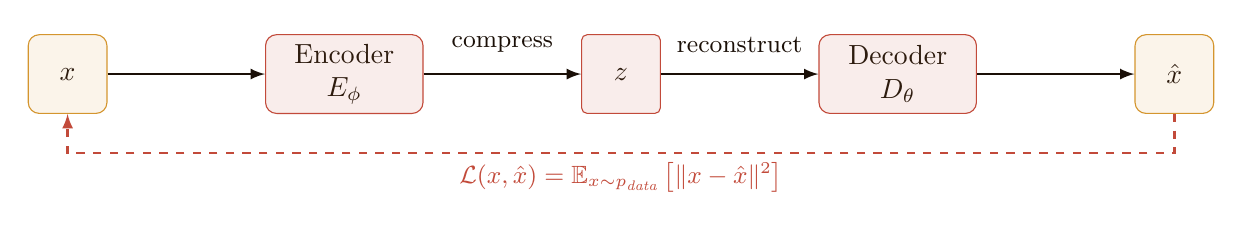
\begin{tikzpicture}[
    node distance=2.0cm, 
    auto, 
    font=\normalsize,
    >=latex
  ]
  
  % Global Style Definitions using your native wp- colors
  \tikzset{
    box/.style={draw=wp-primary, fill=wp-primary!10, rounded corners, minimum width=2.0cm, minimum height=1.0cm, text=wp-text, align=center},
    input/.style={draw=wp-accent, fill=wp-accent!10, rounded corners, minimum width=1.0cm, minimum height=1.0cm, text=wp-text, align=center},
    latent/.style={draw=wp-primary, fill=wp-primary!10, rounded corners=2pt, minimum width=1.0cm, minimum height=1.0cm, text=wp-text, align=center}
  }

  % Horizontal Pipeline
  \node (input)   [input] {$x$};
  \node (encoder) [box, right=of input] {Encoder \\ $E_\phi$};
  \node (latent)  [latent, right=of encoder] {$z$};
  \node (decoder) [box, right=of latent] {Decoder \\ $D_\theta$};
  \node (output)  [input, right=of decoder] {$\hat{x}$};

  % Connecting Edges using your primary theme color (Terracotta)
  \draw[->, wp-dark, thick] (input) -- (encoder);
  \draw[->, wp-dark, thick] (encoder) -- (latent);
  \draw[->, wp-dark, thick] (latent) -- (decoder);
  \draw[->, wp-dark, thick] (decoder) -- (output);

  % Step Metadata Labels (Muted earth tone)
  \node[above=0.15cm, wp-dark, font=\small] at ($(encoder.east)!0.5!(latent.west)$) {compress};
  \node[above=0.15cm, wp-dark, font=\small] at ($(latent.east)!0.5!(decoder.west)$) {reconstruct};

  
  % Desce reto de output, corre horizontalmente e sobe reto para input
  \draw[->, draw=wp-primary, thick, dashed] 
      (output.south) -- ++(0,-0.5) -| (input.south);
      
  % Texto posicionado exatamente no centro do eixo horizontal (alinhado sob o latent)
  \node[wp-primary, font=\itshape\small, below=1.0cm] at (latent.center) 
      {$\mathcal{L}(x, \hat{x}) = \mathbb{E}_{x \sim p_{\text{data}}} \left[ \Vert x - \hat{x} \Vert^2 \right]$};

\end{tikzpicture}
}
\caption{Exemplo clássico da arquitetura de um Autoencoder (AE).}
\label{fig:ae_expanded}
\end{figure*}

\subsection{Espaço Latente}

O espaço latente $\mathcal{Z}$ é uma representação de dimensionalidade reduzida dos dados de entrada. Para cada dado $x \in \mathcal{X}$, o encoder mapeia $x$ para um vetor 
latente $z \in \mathcal{Z}$:

\begin{equation*}
    z = E_{\phi}(x)
\end{equation*}

Esse vetor latente $z$ captura as características essenciais dos dados de entrada, eliminando redundâncias e ruídos.
 A dimensionalidade de $\mathcal{Z}$ é tipicamente menor que a de $\mathcal{X}$, o que permite ao autoencoder aprender uma representação compacta e eficiente.

\subsection{Funcionamento do Autoencoder}

A intuição por trás de um autoencoder pode ser resumida em três etapas principais:
\begin{enumerate}
    \item \textbf{Entrada}: Um dado $x \in \mathbb{R}^D$ é fornecido como entrada.
    \item \textbf{Encoder}: O encoder mapeia $x$ para um vetor latente $z \in \mathbb{R}^d$, onde $d \ll D$:
   \begin{equation*}
       z = E(x) = \sigma(W_e x + b_e)
   \end{equation*}
   Aqui, $W_e$ e $b_e$ são os pesos e vieses do encoder, respectivamente, e $\sigma$ é uma função de ativação não linear (como ReLU ou sigmoide).
   \item $\mathbf{Decoder}$ O decoder reconstrói $\hat{x} \in \mathbb{R}^D$ a partir do vetor latente $z$:
   \begin{equation*}
       \hat{x} = D(z) = \sigma(W_d z + b_d)
   \end{equation*}
   Onde $W_d$ e $b_d$ são os pesos e vieses do decoder.
\end{enumerate}

\subsection{Função de Perda}

O objetivo do autoencoder é minimizar o erro de reconstrução, ou seja, a diferença entre a entrada original $x$ e a reconstrução $\hat{x}$. 
A função de perda mais comum é o erro quadrático médio (MSE), definido como:

\begin{equation*}
    \mathcal{L}_{AE} = \mathbb{E}_{x \sim p_{\text{data}}} \left[ \Vert x - \hat{x} \Vert^2 \right]
\end{equation*}

Onde:
\begin{itemize}
    \item $\mathbb{E}_{x \sim p_{\text{data}}}$ denota o valor esperado em relação à distribuição dos dados de entrada.
    \item $\Vert x - \hat{x} \Vert^2$ é a norma euclidiana ao quadrado da diferença entre $x$ e $\hat{x}$.
\end{itemize}


Ao minimizar essa função de perda, o autoencoder aprende a reconstruir os dados de entrada com a maior precisão possível, ao mesmo tempo em que compacta a informação no espaço latente.

\subsection{Variações de Autoencoders}

Além do autoencoder básico, existem várias variações que ampliam suas capacidades:
\begin{itemize}
    \item Denoising Autoencoder: Treinado para reconstruir dados a partir de entradas corrompidas por ruído.
    \item Sparse Autoencoder: Introduz uma penalidade de esparsidade no espaço latente, incentivando a ativação de apenas algumas unidades latentes.
    \item Variational Autoencoder (VAE): Modela a distribuição dos dados no espaço latente, permitindo a geração de novos dados.
    \item Convolutional Autoencoder: Utiliza camadas convolucionais no encoder e decoder, sendo especialmente útil para dados imagéticos.
\end{itemize}


\section{Variational Autoencoders (VAEs)}

Os Variational Autoencoders (VAEs) são uma extensão dos autoencoders tradicionais que incorporam conceitos de inferência probabilística. 
Enquanto autoencoders comuns aprendem uma representação determinística no espaço latente, os VAEs modelam a distribuição de probabilidade dos dados no espaço latente, permitindo a 
geração de novos dados a partir dessa distribuição. 

\begin{figure*}[htbp]
\centering
\resizebox{\textwidth}{!}{%
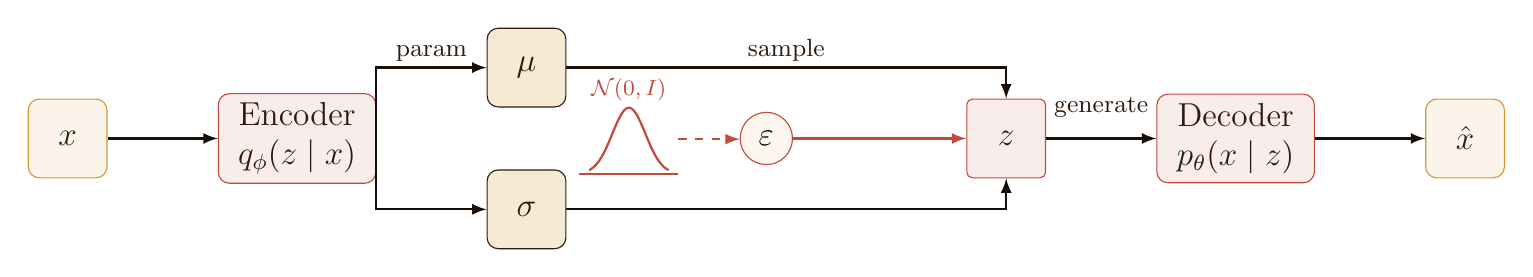
\begin{tikzpicture}[
    node distance=1.0cm and 1.4cm, 
    auto, 
    font=\large,
    >=latex
  ]
  
  % Global Style Definitions matching your exact branding
  \tikzset{    
    box/.style={draw=wp-primary, fill=wp-primary!10, rounded corners, minimum width=2.0cm, minimum height=1.0cm, text=wp-text, align=center},
    input/.style={draw=wp-accent, fill=wp-accent!10, rounded corners, minimum width=1.0cm, minimum height=1.0cm, text=wp-text, align=center},
    latent/.style={draw=wp-primary, fill=wp-primary!10, rounded corners=2pt, minimum width=1.0cm, minimum height=1.0cm, text=wp-text, align=center},
    param/.style={draw=wp-text, fill=wp-accent!20, rounded corners, minimum width=1.0cm, minimum height=1.0cm, text=wp-text, align=center}
  }

  % Pipeline Nodes
  \node (input)   [input] {$x$};
  \node (encoder) [box, right=of input] {Encoder \\ $q_\phi(z \mid x)$};
  
  % Distributed Latent Parameters
  \node (mu)      [param, right=of encoder, yshift=0.9cm] {$\mu$};
  \node (sigma)   [param, right=of encoder, yshift=-0.9cm] {$\sigma$};
  
  \coordinate (gauss_center) at ($(encoder.east)!0.5!(mu.east)$);
  
  % --- EMBEDDED GAUSSIAN BELL CURVE PLOT ---
  \begin{scope}[shift={($(gauss_center)-(-2.0cm,0.9cm)$)}, scale=0.42]
    % Small axis floor
    \draw[wp-primary, thick] (-1.5,0) -- (1.5,0);
    % Plotting the normal distribution function mathematically
    \draw[domain=-1.2:1.2, samples=60, smooth, thick, wp-primary] 
      plot (\x, {2.0*exp(-\x*\x*2)});
    % Small label indicator
    \node[wp-primary, font=\footnotesize, above] at (0, 1.9) {$\mathcal{N}(0,I)$};
    
    % Âncora calibrada no fim do eixo direito (y=0) para perfeito alinhamento horizontal
    \coordinate (borda_direita_gauss) at (1.5, 1.05);
  \end{scope}

  % Reparameterization Ring (Stochastic Noise)
  \node (reparam) [draw=wp-primary, circle, fill=wp-bg, inner sep=4pt, right=of mu, xshift=0.8cm, yshift=-0.9cm] {$\varepsilon$};
  
  % Target Generation Substrate
  \node (z)       [latent, right=of reparam, xshift=0.8cm] {$z$};
  \node (decoder) [box, right=of z] {Decoder \\ $p_\theta(x \mid z)$};
  \node (output)  [input, right=of decoder] {$\hat{x}$};

  % Encoder Out-routing (Orthogonal splits)
  \draw[->, wp-dark, thick] (input) -- (encoder);
  \draw[->, wp-dark, thick] (encoder.east) |- (mu.west);
  \draw[->, wp-dark, thick] (encoder.east) |- (sigma.west);

 % Força a seta a sair da borda da gaussiana e ir perfeitamente reta (0º) até a altura exata do centro de epsilon
  \draw[->, wp-primary, dashed, thick] (borda_direita_gauss) -- (reparam.west |- borda_direita_gauss);

  % Convergence paths tracking into Latent Z
  \draw[->, wp-dark, thick] (mu.east) -| (z.north);
  \draw[->, wp-dark, thick] (sigma.east) -| (z.south);
  \draw[->, wp-primary, thick] (reparam.east) -- (z.west);

  % Generation loop termination
  \draw[->, wp-dark, thick] (z) -- (decoder);
  \draw[->, wp-dark, thick] (decoder) -- (output);

  % Flawless Textual Flow Anchors (Centered mathematically in the blank channels)
  \node[above=0.4cm, wp-text, font=\small] at ($(encoder.east)!0.5!(mu.west)$) {param};
  \node[above=0.15cm, wp-text, font=\small] at ($(mu.east)!0.5!(z.north)$) {sample};
  \node[above=0.15cm, wp-text, font=\small] at ($(z.east)!0.5!(decoder.west)$) {generate};

\end{tikzpicture}
}
\caption{Arquitetura de um Variational Autoencoder (VAE) detalhando o reparameterization trick em formato expandido com amostragem exógena de uma distribuição $\mathcal{N}(0, I)$.}
\label{fig:vae_expanded_final}
\end{figure*}



\subsection{Fundamentos Probabilísticos}

Ao contrário dos autoencoders tradicionais, que mapeiam diretamente uma entrada $x$ para um vetor latente $z$, os VAEs modelam a distribuição de probabilidade $p(z|x)$. No entanto, como essa distribuição é intratável, os VAEs utilizam uma abordagem variacional para aproximá-la. Especificamente, eles introduzem uma distribuição aproximada $q_{\phi}(z|x)$, parametrizada por $\phi$, que é aprendida durante o treinamento.

O objetivo do VAE é maximizar a ELBO, que é uma aproximação do logaritmo da verossimilhança dos dados. A ELBO é dada por:

\begin{equation*}
    \text{ELBO} = \mathbb{E}_{q_{\phi}(z|x)} \left[ \log p_{\theta}(x|z) \right] - D_{\text{KL}}(q_{\phi}(z|x) \Vert p(z))
\end{equation*}

Onde:
\begin{itemize}
\item $\mathbb{E}_{q_{\phi}(z|x)} \left[ \log p_{\theta}(x|z) \right]$ é o termo de reconstrução, que mede quão bem o decoder consegue reconstruir $x$ a partir de $z$.
\item $D_{\text{KL}}(q_{\phi}(z|x) \Vert p(z))$ é a divergência de Kullback-Leibler (KL) entre a distribuição aproximada $q_{\phi}(z|x)$ e uma distribuição pré-definida $p(z)$ (geralmente uma distribuição normal padrão $\mathcal{N}(0, I)$).
\end{itemize}

\subsection{Encoder e Decoder Probabilísticos}

No VAE, tanto o encoder quanto o decoder são modelados probabilisticamente:
\begin{enumerate}
    \item \textbf{Encoder}: O encoder mapeia a entrada $x$ para os parâmetros de uma distribuição no espaço latente, geralmente uma distribuição normal multivariada:
   \begin{equation*}
       q_{\phi}(z|x) = \mathcal{N}(z; \mu_{\phi}(x), \sigma_{\phi}^2(x))
   \end{equation*}
   Onde $\mu_{\phi}(x)$ e $\sigma_{\phi}^2(x)$ são a média e a variância da distribuição, respectivamente, aprendidas pelo encoder.
   \item \textbf{Decoder}: O decoder mapeia o vetor latente $z$ para os parâmetros de uma distribuição nos dados de saída. Para dados contínuos, isso geralmente é uma distribuição normal:
   \begin{equation*}
       p_{\theta}(x|z) = \mathcal{N}(x; \mu_{\theta}(z), \sigma_{\theta}^2(z))
   \end{equation*}
   Para dados binários, uma distribuição Bernoulli pode ser usada.

\end{enumerate} 

\subsection{Reparametrização}

Um desafio no treinamento de VAEs é a amostragem de $z$ a partir de $q_{\phi}(z|x)$, que é uma operação estocástica e não diferenciável. Para contornar esse problema, os VAEs utilizam de reparametrização: em vez de amostrar diretamente de $q_{\phi}(z|x)$, eles amostram de uma distribuição base $\epsilon \sim \mathcal{N}(0, I)$ e transformam a amostra da seguinte forma:

\begin{equation*}
    z = \mu_{\phi}(x) + \sigma_{\phi}(x) \cdot \epsilon
\end{equation*}

Essa transformação torna o processo diferenciável, permitindo o uso de gradientes descendentes para otimizar os parâmetros do modelo.

\subsection{Função de Perda}

A função de perda do VAE é o negativo da ELBO, que consiste em dois termos:
\begin{enumerate}
    \item Termo de reconstrução: Mede a qualidade da reconstrução dos dados de entrada.
    \item Termo de regularização: A divergência KL, que força a distribuição aproximada $q_{\phi}(z|x)$ a se aproximar da distribuição pré-definida $p(z)$.
\end{enumerate}

Matematicamente, a função de perda é dada por:

\begin{equation*}
    \mathcal{L}_{\text{VAE}} = -\mathbb{E}_{q_{\phi}(z|x)} \left[ \log p_{\theta}(x|z) \right] + D_{\text{KL}}(q_{\phi}(z|x) \Vert p(z))
\end{equation*}

\subsection{Exemplo de Arquitetura}

Um VAE típico consiste em:
\begin{enumerate}
    \item Encoder: Uma rede neural que mapeia a entrada $x$ para os parâmetros $\mu_{\phi}(x)$ e $\sigma_{\phi}(x)$ da distribuição latente.
    \item Reparametrização: Amostra $z$ usando o truque da reparametrização.
    \item Decoder: Uma rede neural que mapeia $z$ para os parâmetros da distribuição de saída $p_{\theta}(x|z)$.
\end{enumerate}

\subsection{Vantagens e Desvantagens}

\paragraph{Vantagens}
\begin{itemize}
    \item Permitem a geração de novos dados a partir de uma distribuição aprendida.
    \item O espaço latente é contínuo, o que facilita a interpolação e a manipulação de dados.
    \item São baseados em fundamentos probabilísticos sólidos.
\end{itemize}


\paragraph{Desvantagens}
\begin{itemize}
    \item As amostras geradas podem ser menos nítidas ou realistas em comparação com outras técnicas, como GANs (Generative Adversarial Networks).
    \item O treinamento pode ser mais complexo devido à necessidade de otimizar a ELBO.

\end{itemize}

\section{Generative Adversarial Networks (GANs)}

As Generative Adversarial Networks (GANs) são uma classe de modelos de aprendizado profundo introduzidos por Ian Goodfellow e colaboradores em 2014. Elas são amplamente utilizadas para geração de dados, como imagens, áudio e texto. A ideia central das GANs é treinar dois modelos neurais simultaneamente: um \textbf{gerador} (generator) e um \textbf{discriminador} (discriminator), que competem entre si em um jogo de soma zero. Essa competição leva à geração de dados realistas que são indistinguíveis dos dados reais.

\subsection{Fundamentos das GANs}

Uma GAN consiste em dois componentes principais:
\begin{enumerate}
    \item Gerador ($G$): Um modelo que gera dados a partir de um vetor de ruído aleatório $z$, geralmente amostrado de uma distribuição simples, como uma distribuição normal ou uniforme. O objetivo do gerador é produzir dados que sejam indistinguíveis dos dados reais.
    \item Discriminador ($D$): Um modelo que tenta distinguir entre dados reais (amostrados da distribuição real $p_{\text{data}}(x)$) e dados falsos (gerados pelo gerador). O discriminador é treinado para maximizar a probabilidade de classificar corretamente os dados como reais ou falsos.
\end{enumerate}

% GAN — Arquitetura Otimizada (Texto de Retropropagação Interno e Centralizado)
% Uso: % GAN — Arquitetura Otimizada (Texto de Retropropagação Interno e Centralizado)
% Uso: % GAN — Arquitetura Otimizada (Texto de Retropropagação Interno e Centralizado)
% Uso: \input{resources/gan/gan-architecture.tex}
\begin{figure}[htbp]
\centering
\resizebox{\textwidth}{!}{%
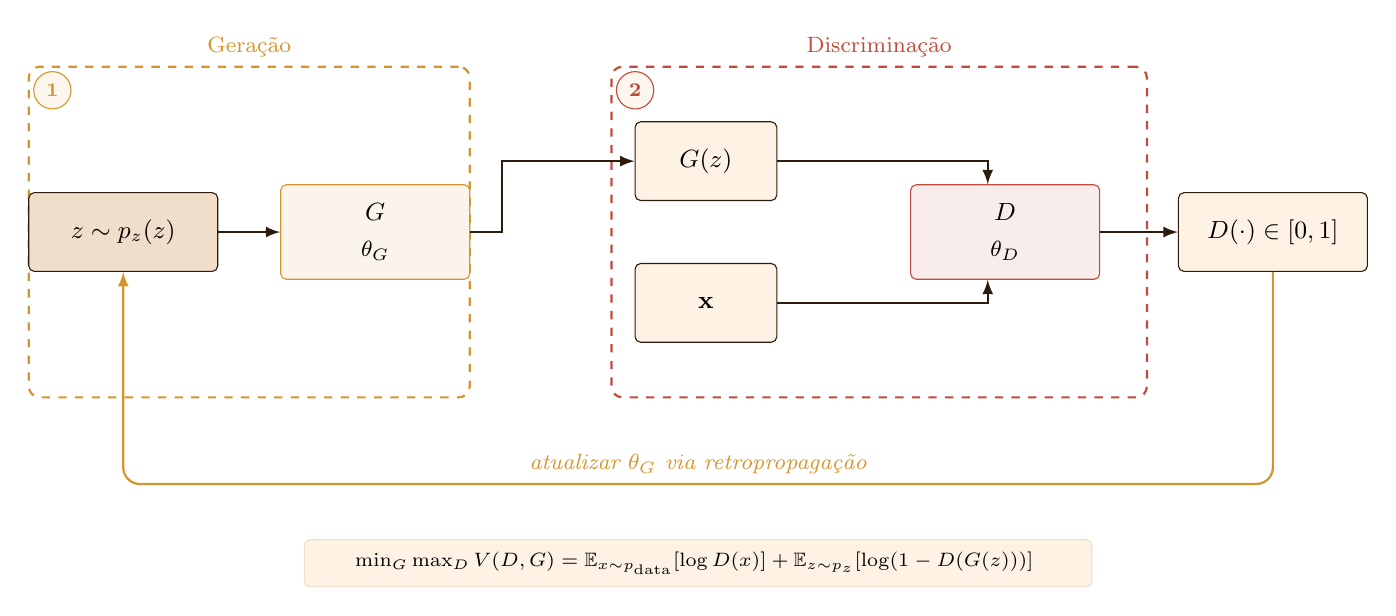
\begin{tikzpicture}[
    >=latex,
    box/.style={draw=wp-text, fill=wp-light, rounded corners=2pt, minimum width=2.4cm, minimum height=1.0cm, align=center, font=\small},
    gen/.style={draw=wp-accent, fill=wp-accent!10, rounded corners=2pt, minimum width=2.4cm, minimum height=1.2cm, align=center, font=\small},
    disc/.style={draw=wp-primary, fill=wp-primary!10, rounded corners=2pt, minimum width=2.4cm, minimum height=1.2cm, align=center, font=\small},
    data/.style={draw=wp-text, fill=wp-code, rounded corners=2pt, minimum width=1.8cm, minimum height=1.0cm, align=center, font=\small},
    conn/.style={->, draw=wp-text, thick},
    label/.style={font=\footnotesize, text=wp-primary},
    tuftebox/.style={draw=wp-light, fill=wp-code, rounded corners=2pt, align=center},
    genbox/.style={draw=wp-accent, dashed, line width=0.8pt, fill=none, rounded corners=4pt, minimum width=5.6cm, minimum height=4.2cm, align=center},
    discbox/.style={draw=wp-primary, dashed, line width=0.8pt, fill=none, rounded corners=4pt, minimum width=6.8cm, minimum height=4.2cm, align=center},
    phase/.style={draw=wp-primary, fill=wp-bg, circle, inner sep=2.5pt, font=\scriptsize\bfseries}
]

% =========================================================================
% FASE 1: GERAÇÃO (Container wp-accent à Esquerda)
% =========================================================================
\node[genbox] (g_container) at (1.6, 0.7) {};
\node[label, above, text=wp-accent] at (g_container.north) {Geração};

\node[box] (z) at (0, 0.7) {$z \sim p_z(z)$};
\node[gen] (G) at (3.2, 0.7) {$G$\\[2pt]\footnotesize$\theta_G$};

\draw[conn] (z) -- (G);


% =========================================================================
% FASE 2: DISCRIMINAÇÃO (Container wp-primary ao Centro)
% =========================================================================
\node[discbox] (d_container) at (9.6, 0.7) {};
\node[label, above, text=wp-primary] at (d_container.north) {Discriminação};

\node[data] (fake) at (7.4, 1.6) {$G(z)$};
\node[data] (real) at (7.4, -0.2) {$\mathbf{x}$};
\node[disc] (D)    at (11.2, 0.7) {$D$\\[2pt]\footnotesize$\theta_D$};

\draw[conn] (G.east) -- ++(0.4,0) |- (fake.west);
\draw[conn] (fake.east) -| (D.110);
\draw[conn] (real.east) -| (D.250);


% =========================================================================
% SAÍDA: AVALIAÇÃO DA PROBABILIDADE (Extrema Direita)
% =========================================================================
\node[box, fill=wp-code, draw=wp-text] (out) at (14.6, 0.7) {$D(\cdot) \in [0,1]$};
\draw[conn] (D) -- (out);


% =========================================================================
% INDICADORES NUMÉRICOS DAS FASES
% =========================================================================
\node[phase, text=wp-accent, draw=wp-accent] at (-0.9, 2.5) {1};
\node[phase, text=wp-primary, draw=wp-primary] at (6.5, 2.5) {2};


% =========================================================================
% FEEDBACK LOOP (Seta Externa de Retorno)
% =========================================================================
\draw[->, draw=wp-accent, thick, rounded corners=6pt] 
    (out.south) -- (14.6, -2.5) -- (0, -2.5) -- (z.south);

% AJUSTE: Centralizado em x=7.3 e jogado para o lado de dentro (anchor=south)
\node[font=\itshape\footnotesize, text=wp-accent, anchor=south] at (7.3, -2.5) 
    {atualizar $\theta_G$ via retropropagação};


% =========================================================================
% EQUAÇÃO DE LOSS CENTRALIZADA NA BASE
% =========================================================================
\node[tuftebox, minimum width=10.0cm, minimum height=0.6cm, inner sep=4pt, anchor=north] at (7.3, -3.2) {
    \scriptsize $\min_G \max_D V(D,G) = \mathbb{E}_{x \sim p_{\text{data}}}[\log D(x)] + \mathbb{E}_{z \sim p_z}[\log(1-D(G(z)))]$
};

\end{tikzpicture}
}
\caption{Arquitetura de uma GAN. Jogo adversarial de soma zero entre o gerador $G$ e o discriminador $D$.}
\label{fig:gan-architecture}
\end{figure}
\begin{figure}[htbp]
\centering
\resizebox{\textwidth}{!}{%
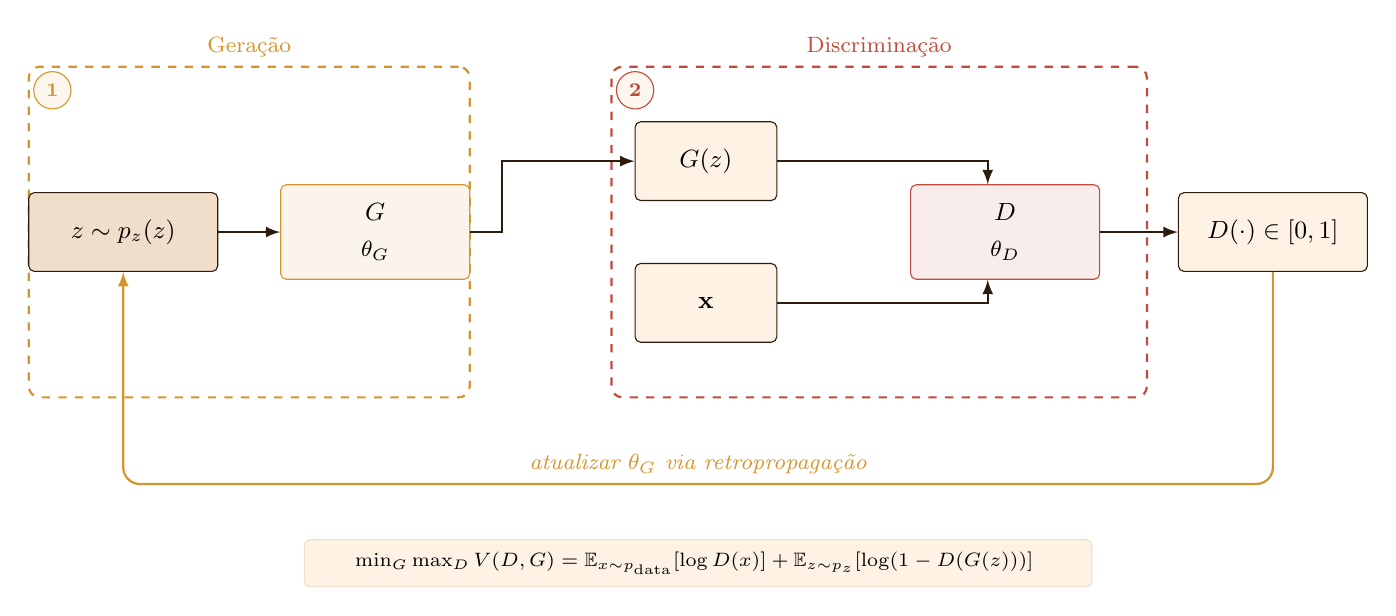
\begin{tikzpicture}[
    >=latex,
    box/.style={draw=wp-text, fill=wp-light, rounded corners=2pt, minimum width=2.4cm, minimum height=1.0cm, align=center, font=\small},
    gen/.style={draw=wp-accent, fill=wp-accent!10, rounded corners=2pt, minimum width=2.4cm, minimum height=1.2cm, align=center, font=\small},
    disc/.style={draw=wp-primary, fill=wp-primary!10, rounded corners=2pt, minimum width=2.4cm, minimum height=1.2cm, align=center, font=\small},
    data/.style={draw=wp-text, fill=wp-code, rounded corners=2pt, minimum width=1.8cm, minimum height=1.0cm, align=center, font=\small},
    conn/.style={->, draw=wp-text, thick},
    label/.style={font=\footnotesize, text=wp-primary},
    tuftebox/.style={draw=wp-light, fill=wp-code, rounded corners=2pt, align=center},
    genbox/.style={draw=wp-accent, dashed, line width=0.8pt, fill=none, rounded corners=4pt, minimum width=5.6cm, minimum height=4.2cm, align=center},
    discbox/.style={draw=wp-primary, dashed, line width=0.8pt, fill=none, rounded corners=4pt, minimum width=6.8cm, minimum height=4.2cm, align=center},
    phase/.style={draw=wp-primary, fill=wp-bg, circle, inner sep=2.5pt, font=\scriptsize\bfseries}
]

% =========================================================================
% FASE 1: GERAÇÃO (Container wp-accent à Esquerda)
% =========================================================================
\node[genbox] (g_container) at (1.6, 0.7) {};
\node[label, above, text=wp-accent] at (g_container.north) {Geração};

\node[box] (z) at (0, 0.7) {$z \sim p_z(z)$};
\node[gen] (G) at (3.2, 0.7) {$G$\\[2pt]\footnotesize$\theta_G$};

\draw[conn] (z) -- (G);


% =========================================================================
% FASE 2: DISCRIMINAÇÃO (Container wp-primary ao Centro)
% =========================================================================
\node[discbox] (d_container) at (9.6, 0.7) {};
\node[label, above, text=wp-primary] at (d_container.north) {Discriminação};

\node[data] (fake) at (7.4, 1.6) {$G(z)$};
\node[data] (real) at (7.4, -0.2) {$\mathbf{x}$};
\node[disc] (D)    at (11.2, 0.7) {$D$\\[2pt]\footnotesize$\theta_D$};

\draw[conn] (G.east) -- ++(0.4,0) |- (fake.west);
\draw[conn] (fake.east) -| (D.110);
\draw[conn] (real.east) -| (D.250);


% =========================================================================
% SAÍDA: AVALIAÇÃO DA PROBABILIDADE (Extrema Direita)
% =========================================================================
\node[box, fill=wp-code, draw=wp-text] (out) at (14.6, 0.7) {$D(\cdot) \in [0,1]$};
\draw[conn] (D) -- (out);


% =========================================================================
% INDICADORES NUMÉRICOS DAS FASES
% =========================================================================
\node[phase, text=wp-accent, draw=wp-accent] at (-0.9, 2.5) {1};
\node[phase, text=wp-primary, draw=wp-primary] at (6.5, 2.5) {2};


% =========================================================================
% FEEDBACK LOOP (Seta Externa de Retorno)
% =========================================================================
\draw[->, draw=wp-accent, thick, rounded corners=6pt] 
    (out.south) -- (14.6, -2.5) -- (0, -2.5) -- (z.south);

% AJUSTE: Centralizado em x=7.3 e jogado para o lado de dentro (anchor=south)
\node[font=\itshape\footnotesize, text=wp-accent, anchor=south] at (7.3, -2.5) 
    {atualizar $\theta_G$ via retropropagação};


% =========================================================================
% EQUAÇÃO DE LOSS CENTRALIZADA NA BASE
% =========================================================================
\node[tuftebox, minimum width=10.0cm, minimum height=0.6cm, inner sep=4pt, anchor=north] at (7.3, -3.2) {
    \scriptsize $\min_G \max_D V(D,G) = \mathbb{E}_{x \sim p_{\text{data}}}[\log D(x)] + \mathbb{E}_{z \sim p_z}[\log(1-D(G(z)))]$
};

\end{tikzpicture}
}
\caption{Arquitetura de uma GAN. Jogo adversarial de soma zero entre o gerador $G$ e o discriminador $D$.}
\label{fig:gan-architecture}
\end{figure}
\begin{figure}[htbp]
\centering
\resizebox{\textwidth}{!}{%
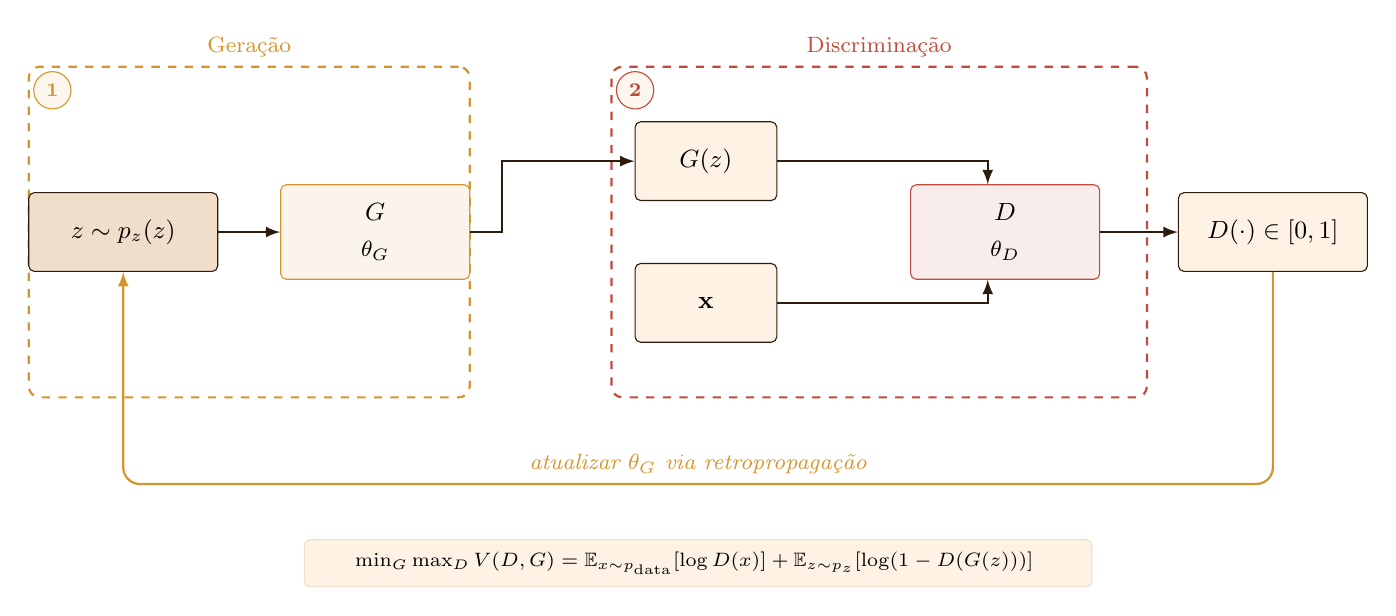
\begin{tikzpicture}[
    >=latex,
    box/.style={draw=wp-text, fill=wp-light, rounded corners=2pt, minimum width=2.4cm, minimum height=1.0cm, align=center, font=\small},
    gen/.style={draw=wp-accent, fill=wp-accent!10, rounded corners=2pt, minimum width=2.4cm, minimum height=1.2cm, align=center, font=\small},
    disc/.style={draw=wp-primary, fill=wp-primary!10, rounded corners=2pt, minimum width=2.4cm, minimum height=1.2cm, align=center, font=\small},
    data/.style={draw=wp-text, fill=wp-code, rounded corners=2pt, minimum width=1.8cm, minimum height=1.0cm, align=center, font=\small},
    conn/.style={->, draw=wp-text, thick},
    label/.style={font=\footnotesize, text=wp-primary},
    tuftebox/.style={draw=wp-light, fill=wp-code, rounded corners=2pt, align=center},
    genbox/.style={draw=wp-accent, dashed, line width=0.8pt, fill=none, rounded corners=4pt, minimum width=5.6cm, minimum height=4.2cm, align=center},
    discbox/.style={draw=wp-primary, dashed, line width=0.8pt, fill=none, rounded corners=4pt, minimum width=6.8cm, minimum height=4.2cm, align=center},
    phase/.style={draw=wp-primary, fill=wp-bg, circle, inner sep=2.5pt, font=\scriptsize\bfseries}
]

% =========================================================================
% FASE 1: GERAÇÃO (Container wp-accent à Esquerda)
% =========================================================================
\node[genbox] (g_container) at (1.6, 0.7) {};
\node[label, above, text=wp-accent] at (g_container.north) {Geração};

\node[box] (z) at (0, 0.7) {$z \sim p_z(z)$};
\node[gen] (G) at (3.2, 0.7) {$G$\\[2pt]\footnotesize$\theta_G$};

\draw[conn] (z) -- (G);


% =========================================================================
% FASE 2: DISCRIMINAÇÃO (Container wp-primary ao Centro)
% =========================================================================
\node[discbox] (d_container) at (9.6, 0.7) {};
\node[label, above, text=wp-primary] at (d_container.north) {Discriminação};

\node[data] (fake) at (7.4, 1.6) {$G(z)$};
\node[data] (real) at (7.4, -0.2) {$\mathbf{x}$};
\node[disc] (D)    at (11.2, 0.7) {$D$\\[2pt]\footnotesize$\theta_D$};

\draw[conn] (G.east) -- ++(0.4,0) |- (fake.west);
\draw[conn] (fake.east) -| (D.110);
\draw[conn] (real.east) -| (D.250);


% =========================================================================
% SAÍDA: AVALIAÇÃO DA PROBABILIDADE (Extrema Direita)
% =========================================================================
\node[box, fill=wp-code, draw=wp-text] (out) at (14.6, 0.7) {$D(\cdot) \in [0,1]$};
\draw[conn] (D) -- (out);


% =========================================================================
% INDICADORES NUMÉRICOS DAS FASES
% =========================================================================
\node[phase, text=wp-accent, draw=wp-accent] at (-0.9, 2.5) {1};
\node[phase, text=wp-primary, draw=wp-primary] at (6.5, 2.5) {2};


% =========================================================================
% FEEDBACK LOOP (Seta Externa de Retorno)
% =========================================================================
\draw[->, draw=wp-accent, thick, rounded corners=6pt] 
    (out.south) -- (14.6, -2.5) -- (0, -2.5) -- (z.south);

% AJUSTE: Centralizado em x=7.3 e jogado para o lado de dentro (anchor=south)
\node[font=\itshape\footnotesize, text=wp-accent, anchor=south] at (7.3, -2.5) 
    {atualizar $\theta_G$ via retropropagação};


% =========================================================================
% EQUAÇÃO DE LOSS CENTRALIZADA NA BASE
% =========================================================================
\node[tuftebox, minimum width=10.0cm, minimum height=0.6cm, inner sep=4pt, anchor=north] at (7.3, -3.2) {
    \scriptsize $\min_G \max_D V(D,G) = \mathbb{E}_{x \sim p_{\text{data}}}[\log D(x)] + \mathbb{E}_{z \sim p_z}[\log(1-D(G(z)))]$
};

\end{tikzpicture}
}
\caption{Arquitetura de uma GAN. Jogo adversarial de soma zero entre o gerador $G$ e o discriminador $D$.}
\label{fig:gan-architecture}
\end{figure}

O treinamento das GANs é formulado como um jogo minimax entre o gerador e o discriminador, onde o gerador tenta enganar o discriminador, e o discriminador tenta detectar as amostras falsas. Matematicamente, o objetivo pode ser expresso como:

\begin{equation*}
    \min_G \max_D V(D, G) = \mathbb{E}_{x \sim p_{\text{data}}(x)} \left[ \log D(x) \right] + \mathbb{E}_{z \sim p_z(z)} \left[ \log (1 - D(G(z))) \right]
\end{equation*}

Onde:
\begin{itemize}
    \item $D(x)$ é a probabilidade estimada pelo discriminador de que $x$ seja real.
    \item $G(z)$ é a amostra gerada pelo gerador a partir do vetor de ruído $z$.
    \item $p_{\text{data}}(x)$ é a distribuição dos dados reais.
    \item $p_z(z)$ é a distribuição do vetor de ruído (geralmente $\mathcal{N}(0, I)$ ou $\text{Uniform}(-1, 1)$).
\end{itemize}

\subsection{Funcionamento do Treinamento}

O treinamento de uma GAN envolve as seguintes etapas iterativas:
\begin{enumerate}
    \item Treinamento do Discriminador: Fixa-se o gerador e atualiza-se o discriminador para maximizar a função de custo $V(D, G)$. Isso envolve:
    \begin{itemize}
        \item Classificar corretamente os dados reais como reais.
        \item Classificar corretamente os dados falsos (gerados pelo gerador) como falsos.
    \end{itemize}
    \item Treinamento do Gerador: Fixa-se o discriminador e atualiza-se o gerador para minimizar a função de custo $V(D, G)$. Isso envolve:
    \begin{itemize}
        \item Gerar dados que sejam classificados como reais pelo discriminador.

    \end{itemize}
\end{enumerate}
Esse processo é repetido até que o gerador produza dados realistas e o discriminador não consiga distinguir entre dados reais e falsos.

% GAN — Ciclo de Treinamento NATIVO TUFTE
% Uso: % GAN — Ciclo de Treinamento NATIVO TUFTE
% Uso: % GAN — Ciclo de Treinamento NATIVO TUFTE
% Uso: \input{resources/gan/gan-training-cycle.tex}
\begin{figure}[htbp]
\centering
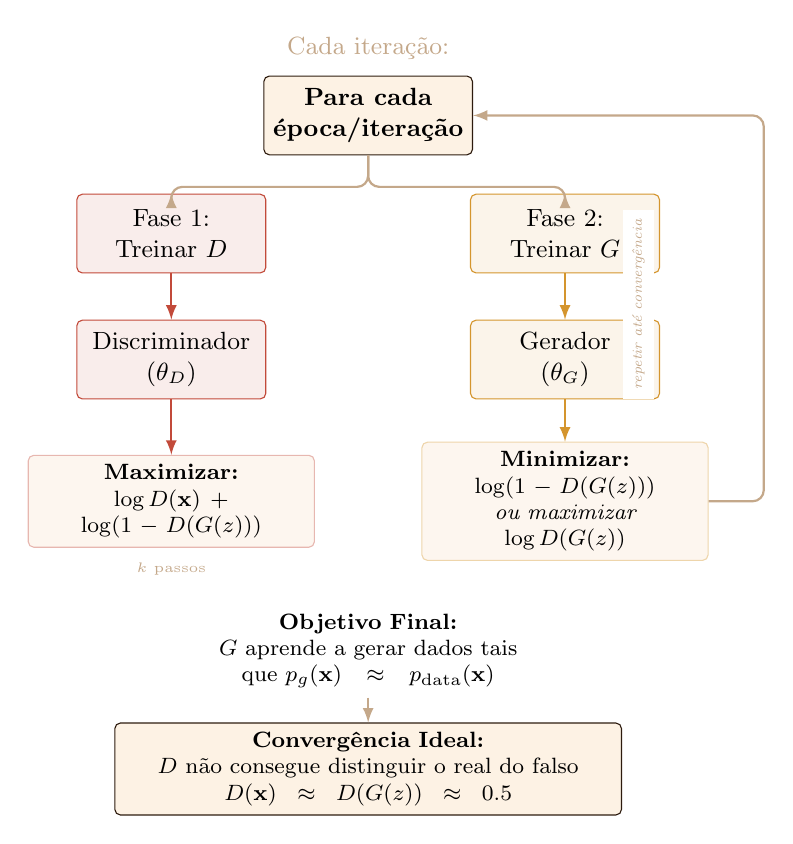
\begin{tikzpicture}[
    >=latex,
    phase/.style={draw=wp-text, fill=wp-code, rounded corners=2pt, minimum width=2.4cm, minimum height=1.0cm, align=center, font=\small},
    modelD/.style={draw=wp-primary, fill=wp-primary!10, rounded corners=2pt, minimum width=2.4cm, minimum height=1.0cm, align=center, font=\small},
    modelG/.style={draw=wp-accent, fill=wp-accent!10, rounded corners=2pt, minimum width=2.4cm, minimum height=1.0cm, align=center, font=\small},
    result/.style={draw=wp-light, fill=wp-bg, rounded corners=2pt, align=center, font=\footnotesize, text width=3.4cm},
    conn/.style={->, thick, draw=wp-text!70}
]

% ── Cabeçalho / Loop Principal ────────────────────────────────
\node[phase, font=\bfseries\small] (loop) at (3.0, 2.5) {Para cada\\época/iteração};
\node[font=\small, wp-muted, anchor=south] at (3.0, 3.1) {Cada iteração:};

% ── Coluna da Esquerda (Fase 1: Discriminador - wp-primary) ───
\node[draw=wp-primary, fill=wp-primary!10, rounded corners=2pt, minimum width=2.4cm, minimum height=1.0cm, align=center, font=\small] (p1) at (0.5, 1.0) {Fase 1:\\Treinar $D$};
\node[modelD] (d1) at (0.5, -0.6) {Discriminador\\($\theta_D$)};
\node[result, draw=wp-primary!40] (r1) at (0.5, -2.4) {\textbf{Maximizar:}\\$\log D(\mathbf{x}) + \log(1 - D(G(z)))$};

\draw[conn, draw=wp-primary] (p1) -- (d1);
\draw[conn, draw=wp-primary] (d1) -- (r1);
\node[font=\tiny, wp-muted, below=2pt] at (r1.south) {$k$ passos};

% ── Coluna da Direita (Fase 2: Gerador - wp-accent) ───────────
\node[draw=wp-accent, fill=wp-accent!10, rounded corners=2pt, minimum width=2.4cm, minimum height=1.0cm, align=center, font=\small] (p2) at (5.5, 1.0) {Fase 2:\\Treinar $G$};
\node[modelG] (g1) at (5.5, -0.6) {Gerador\\($\theta_G$)};
\node[result, draw=wp-accent!40] (r2) at (5.5, -2.4) {\textbf{Minimizar:}\\$\log(1 - D(G(z)))$\\\textit{ou maximizar} $\log D(G(z))$};

\draw[conn, draw=wp-accent] (p2) -- (g1);
\draw[conn, draw=wp-accent] (g1) -- (r2);

% ── Seta de Divisão Inicial do Loop ───────────────────────────
\draw[->, thick, draw=wp-muted, rounded corners=4pt] (loop.south) -- ++(0, -0.4) -| (p1.north);
\draw[->, thick, draw=wp-muted, rounded corners=4pt] (loop.south) -- ++(0, -0.4) -| (p2.north);

% ── Seta de Retorno / Feedback de Progresso (Sem Cruzamento) ──
\draw[->, thick, draw=wp-muted, rounded corners=4pt] (r2.east) -- ++(0.7, 0) |- (loop.east);
\node[font=\itshape\tiny, wp-muted, fill=white, anchor=mid, rotate=90] at (6.4, 0.1) {repetir até convergência};

% =========================================================================
% SEÇÃO DE CONVERGÊNCIA (Bloco de Saída Inferior)
% =========================================================================
\node[font=\footnotesize, align=center, text width=6.5cm] (obj) at (3.0, -4.3) {
    \textbf{Objetivo Final:}\\
    $G$ aprende a gerar dados tais que $p_g(\mathbf{x}) \approx p_{\mathrm{data}}(\mathbf{x})$
};

\node[draw=wp-text, fill=wp-code, rounded corners=2pt, font=\footnotesize, align=center, text width=6.2cm] (conv) at (3.0, -5.8) {
    \textbf{Convergência Ideal:}\\
    $D$ não consegue distinguir o real do falso\\
    $D(\mathbf{x}) \approx D(G(z)) \approx 0.5$
};

\draw[->, draw=wp-muted, thick] (obj.south) -- (conv.north);

\end{tikzpicture}
\caption{Ciclo de treinamento de uma GAN. O processo alterna iterativamente entre a otimização do Discriminador $D$ (Fase 1) e do Gerador $G$ (Fase 2) até que o sistema atinja o equilíbrio de Nash, onde as amostras sintéticas tornam-se indistinguíveis das reais.}
\label{fig:gan-training-cycle}
\end{figure}
\begin{figure}[htbp]
\centering
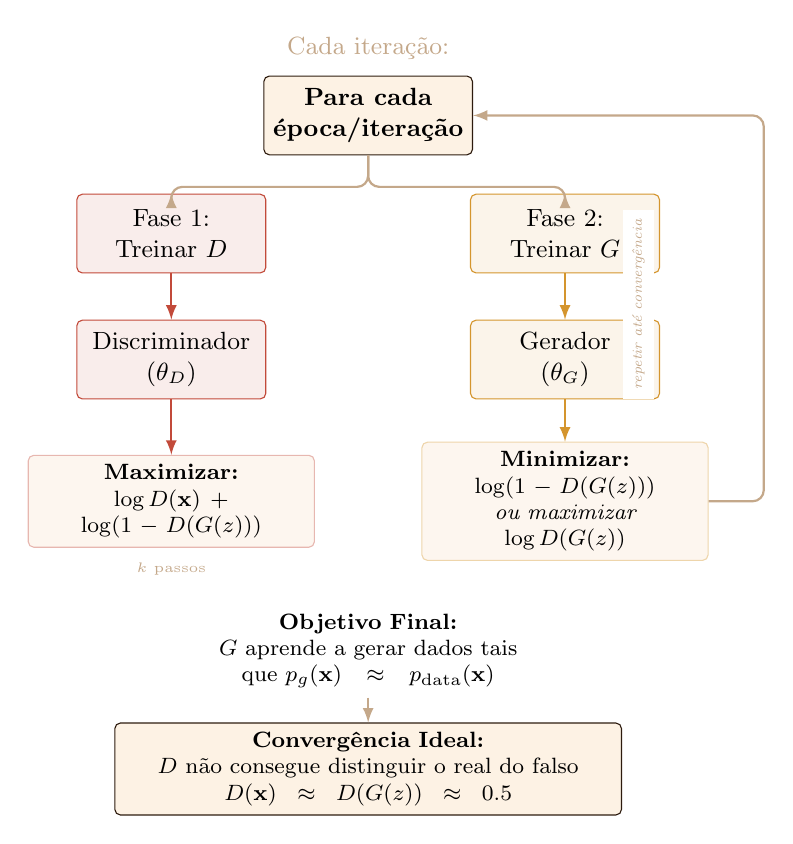
\begin{tikzpicture}[
    >=latex,
    phase/.style={draw=wp-text, fill=wp-code, rounded corners=2pt, minimum width=2.4cm, minimum height=1.0cm, align=center, font=\small},
    modelD/.style={draw=wp-primary, fill=wp-primary!10, rounded corners=2pt, minimum width=2.4cm, minimum height=1.0cm, align=center, font=\small},
    modelG/.style={draw=wp-accent, fill=wp-accent!10, rounded corners=2pt, minimum width=2.4cm, minimum height=1.0cm, align=center, font=\small},
    result/.style={draw=wp-light, fill=wp-bg, rounded corners=2pt, align=center, font=\footnotesize, text width=3.4cm},
    conn/.style={->, thick, draw=wp-text!70}
]

% ── Cabeçalho / Loop Principal ────────────────────────────────
\node[phase, font=\bfseries\small] (loop) at (3.0, 2.5) {Para cada\\época/iteração};
\node[font=\small, wp-muted, anchor=south] at (3.0, 3.1) {Cada iteração:};

% ── Coluna da Esquerda (Fase 1: Discriminador - wp-primary) ───
\node[draw=wp-primary, fill=wp-primary!10, rounded corners=2pt, minimum width=2.4cm, minimum height=1.0cm, align=center, font=\small] (p1) at (0.5, 1.0) {Fase 1:\\Treinar $D$};
\node[modelD] (d1) at (0.5, -0.6) {Discriminador\\($\theta_D$)};
\node[result, draw=wp-primary!40] (r1) at (0.5, -2.4) {\textbf{Maximizar:}\\$\log D(\mathbf{x}) + \log(1 - D(G(z)))$};

\draw[conn, draw=wp-primary] (p1) -- (d1);
\draw[conn, draw=wp-primary] (d1) -- (r1);
\node[font=\tiny, wp-muted, below=2pt] at (r1.south) {$k$ passos};

% ── Coluna da Direita (Fase 2: Gerador - wp-accent) ───────────
\node[draw=wp-accent, fill=wp-accent!10, rounded corners=2pt, minimum width=2.4cm, minimum height=1.0cm, align=center, font=\small] (p2) at (5.5, 1.0) {Fase 2:\\Treinar $G$};
\node[modelG] (g1) at (5.5, -0.6) {Gerador\\($\theta_G$)};
\node[result, draw=wp-accent!40] (r2) at (5.5, -2.4) {\textbf{Minimizar:}\\$\log(1 - D(G(z)))$\\\textit{ou maximizar} $\log D(G(z))$};

\draw[conn, draw=wp-accent] (p2) -- (g1);
\draw[conn, draw=wp-accent] (g1) -- (r2);

% ── Seta de Divisão Inicial do Loop ───────────────────────────
\draw[->, thick, draw=wp-muted, rounded corners=4pt] (loop.south) -- ++(0, -0.4) -| (p1.north);
\draw[->, thick, draw=wp-muted, rounded corners=4pt] (loop.south) -- ++(0, -0.4) -| (p2.north);

% ── Seta de Retorno / Feedback de Progresso (Sem Cruzamento) ──
\draw[->, thick, draw=wp-muted, rounded corners=4pt] (r2.east) -- ++(0.7, 0) |- (loop.east);
\node[font=\itshape\tiny, wp-muted, fill=white, anchor=mid, rotate=90] at (6.4, 0.1) {repetir até convergência};

% =========================================================================
% SEÇÃO DE CONVERGÊNCIA (Bloco de Saída Inferior)
% =========================================================================
\node[font=\footnotesize, align=center, text width=6.5cm] (obj) at (3.0, -4.3) {
    \textbf{Objetivo Final:}\\
    $G$ aprende a gerar dados tais que $p_g(\mathbf{x}) \approx p_{\mathrm{data}}(\mathbf{x})$
};

\node[draw=wp-text, fill=wp-code, rounded corners=2pt, font=\footnotesize, align=center, text width=6.2cm] (conv) at (3.0, -5.8) {
    \textbf{Convergência Ideal:}\\
    $D$ não consegue distinguir o real do falso\\
    $D(\mathbf{x}) \approx D(G(z)) \approx 0.5$
};

\draw[->, draw=wp-muted, thick] (obj.south) -- (conv.north);

\end{tikzpicture}
\caption{Ciclo de treinamento de uma GAN. O processo alterna iterativamente entre a otimização do Discriminador $D$ (Fase 1) e do Gerador $G$ (Fase 2) até que o sistema atinja o equilíbrio de Nash, onde as amostras sintéticas tornam-se indistinguíveis das reais.}
\label{fig:gan-training-cycle}
\end{figure}
\begin{figure}[htbp]
\centering
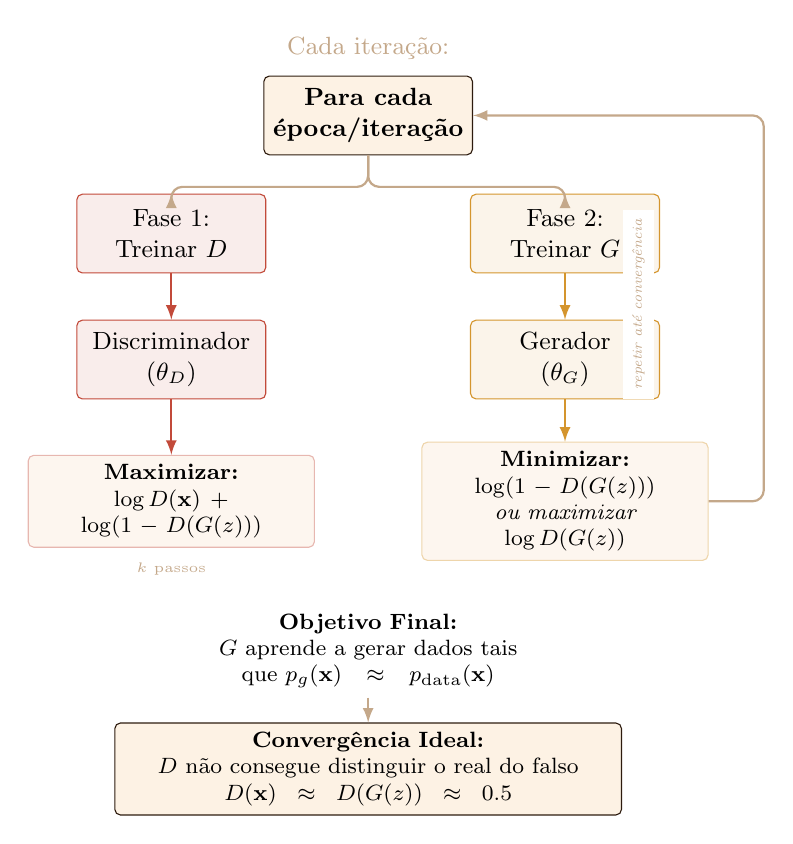
\begin{tikzpicture}[
    >=latex,
    phase/.style={draw=wp-text, fill=wp-code, rounded corners=2pt, minimum width=2.4cm, minimum height=1.0cm, align=center, font=\small},
    modelD/.style={draw=wp-primary, fill=wp-primary!10, rounded corners=2pt, minimum width=2.4cm, minimum height=1.0cm, align=center, font=\small},
    modelG/.style={draw=wp-accent, fill=wp-accent!10, rounded corners=2pt, minimum width=2.4cm, minimum height=1.0cm, align=center, font=\small},
    result/.style={draw=wp-light, fill=wp-bg, rounded corners=2pt, align=center, font=\footnotesize, text width=3.4cm},
    conn/.style={->, thick, draw=wp-text!70}
]

% ── Cabeçalho / Loop Principal ────────────────────────────────
\node[phase, font=\bfseries\small] (loop) at (3.0, 2.5) {Para cada\\época/iteração};
\node[font=\small, wp-muted, anchor=south] at (3.0, 3.1) {Cada iteração:};

% ── Coluna da Esquerda (Fase 1: Discriminador - wp-primary) ───
\node[draw=wp-primary, fill=wp-primary!10, rounded corners=2pt, minimum width=2.4cm, minimum height=1.0cm, align=center, font=\small] (p1) at (0.5, 1.0) {Fase 1:\\Treinar $D$};
\node[modelD] (d1) at (0.5, -0.6) {Discriminador\\($\theta_D$)};
\node[result, draw=wp-primary!40] (r1) at (0.5, -2.4) {\textbf{Maximizar:}\\$\log D(\mathbf{x}) + \log(1 - D(G(z)))$};

\draw[conn, draw=wp-primary] (p1) -- (d1);
\draw[conn, draw=wp-primary] (d1) -- (r1);
\node[font=\tiny, wp-muted, below=2pt] at (r1.south) {$k$ passos};

% ── Coluna da Direita (Fase 2: Gerador - wp-accent) ───────────
\node[draw=wp-accent, fill=wp-accent!10, rounded corners=2pt, minimum width=2.4cm, minimum height=1.0cm, align=center, font=\small] (p2) at (5.5, 1.0) {Fase 2:\\Treinar $G$};
\node[modelG] (g1) at (5.5, -0.6) {Gerador\\($\theta_G$)};
\node[result, draw=wp-accent!40] (r2) at (5.5, -2.4) {\textbf{Minimizar:}\\$\log(1 - D(G(z)))$\\\textit{ou maximizar} $\log D(G(z))$};

\draw[conn, draw=wp-accent] (p2) -- (g1);
\draw[conn, draw=wp-accent] (g1) -- (r2);

% ── Seta de Divisão Inicial do Loop ───────────────────────────
\draw[->, thick, draw=wp-muted, rounded corners=4pt] (loop.south) -- ++(0, -0.4) -| (p1.north);
\draw[->, thick, draw=wp-muted, rounded corners=4pt] (loop.south) -- ++(0, -0.4) -| (p2.north);

% ── Seta de Retorno / Feedback de Progresso (Sem Cruzamento) ──
\draw[->, thick, draw=wp-muted, rounded corners=4pt] (r2.east) -- ++(0.7, 0) |- (loop.east);
\node[font=\itshape\tiny, wp-muted, fill=white, anchor=mid, rotate=90] at (6.4, 0.1) {repetir até convergência};

% =========================================================================
% SEÇÃO DE CONVERGÊNCIA (Bloco de Saída Inferior)
% =========================================================================
\node[font=\footnotesize, align=center, text width=6.5cm] (obj) at (3.0, -4.3) {
    \textbf{Objetivo Final:}\\
    $G$ aprende a gerar dados tais que $p_g(\mathbf{x}) \approx p_{\mathrm{data}}(\mathbf{x})$
};

\node[draw=wp-text, fill=wp-code, rounded corners=2pt, font=\footnotesize, align=center, text width=6.2cm] (conv) at (3.0, -5.8) {
    \textbf{Convergência Ideal:}\\
    $D$ não consegue distinguir o real do falso\\
    $D(\mathbf{x}) \approx D(G(z)) \approx 0.5$
};

\draw[->, draw=wp-muted, thick] (obj.south) -- (conv.north);

\end{tikzpicture}
\caption{Ciclo de treinamento de uma GAN. O processo alterna iterativamente entre a otimização do Discriminador $D$ (Fase 1) e do Gerador $G$ (Fase 2) até que o sistema atinja o equilíbrio de Nash, onde as amostras sintéticas tornam-se indistinguíveis das reais.}
\label{fig:gan-training-cycle}
\end{figure}

\subsection{Funções de Perda}

A função de perda das GANs pode ser interpretada como uma medida de divergência entre a distribuição real $p_{\text{data}}(x)$ e a distribuição gerada $p_g(x)$. No entanto, o treinamento das GANs é conhecido por ser instável, o que levou ao desenvolvimento de várias variações e funções de perda alternativas, como:
\begin{itemize}
    \item GAN Padrão: Usa a função de perda binária cruzada (binary cross-entropy).
    \item Wasserstein GAN (WGAN): Utiliza a distância de Wasserstein para melhorar a estabilidade do treinamento.
    \item Least Squares GAN (LSGAN): Substitui a função de perda binária cruzada por uma função de perda quadrática.    
\end{itemize}

% GAN Mode Collapse Diagram — Tufte & Official Warm Style
% Uso: % GAN Mode Collapse Diagram — Tufte & Official Warm Style
% Uso: % GAN Mode Collapse Diagram — Tufte & Official Warm Style
% Uso: \input{resources/gan/gan-mode-collapse.tex}
\begin{figure}[htbp]
\centering
\resizebox{\textwidth}{!}{%
\begin{tikzpicture}[
    >=latex,
    axis/.style={->, thick, draw=wp-muted},
    % Usando suas cores oficiais com opacidade calibrada para o fundo wp-bg
    realcolor/.style={draw=wp-accent, thick, fill=wp-accent!20},
    gencolor/.style={draw=wp-primary, thick, fill=wp-primary!20},
    tuftebox/.style={draw=wp-light, fill=wp-code, rounded corners=2pt, align=center, font=\small}
]

% =========================================================================
% PARTE SUPERIOR: DISTRIBUIÇÃO REAL (MULTIMODAL EXPANDIDA)
% =========================================================================

% Eixo Real Expandido para 11.0
\draw[axis] (0,0) -- (11,0) node[right, font=\normalsize, text=wp-text] {$x$};
\node[anchor=west, wp-accent, font=\bfseries\normalsize] at (0,2.5) {Distribuição Real $p_{\text{data}}(x)$};

% Modos espaçados horizontalmente (com preenchimento wp-accent)
\foreach \x/\num in {1.2/1, 3.2/2, 5.2/3, 7.2/4, 9.2/5} {
    \draw[realcolor] (\x-0.5,0) .. controls (\x-0.1,0) and (\x-0.1,1.8) .. (\x,1.8) 
                          .. controls (\x+0.1,1.8) and (\x+0.1,0) .. (\x+0.5,0);
    \node[above, font=\small, text=wp-muted] at (\x, 1.8) {Modo \num};
}

% Bloco Desejado Minimalista empurrado para a direita (x = 14.5, y = 0.9)
\node[tuftebox, minimum width=3.8cm, minimum height=2.4cm] (desejado) at (14.5, 0.9) {
    \textbf{\color{wp-accent}Comportamento Desejado}\\
    \small Gerador aprende todos os modos\\[6pt]
    \begin{tikzpicture}[scale=0.35]
        \foreach \x in {1,...,5} \draw[fill=wp-accent!60, draw=wp-accent] (\x,0) circle (0.25);
    \end{tikzpicture}\\
    \footnotesize\color{wp-muted}Amostras diversas (0, 1, 2, 3, 4...)
};

\draw[->, dashed, draw=wp-muted] (10.5,0.7) -- (desejado.west);


% =========================================================================
% TEXTO EXPLICATIVO INTERMEDIÁRIO (Nota editorial Tufte, sem caixa)
% =========================================================================
\node[font=\itshape\small, text=wp-text, text width=9.0cm] at (4.2, -0.7) {
    O gerador $G$ explora uma região limitada do espaço que consegue enganar o discriminador $D$ com mais facilidade.
};


% =========================================================================
% PARTE INFERIOR: COLAPSO DE MODO (Alinhamento Vertical Corrigido)
% =========================================================================

% Eixo Gerado posicionado em y = -4.5
\draw[axis] (0,-4.5) -- (11,-4.5) node[right, font=\small, text=wp-text] {$x$};

% Título posicionado com segurança em y = -2.0 (acima do pico)
\node[anchor=west, wp-primary, font=\bfseries\small] at (0,-2.0) {Distribuição Gerada $p_g(x)$ $\rightarrow$ Colapso};

% Modo único alinhado perfeitamente com o Modo 3 (x = 5.2). Preenchimento wp-primary
\draw[gencolor, line width=1pt] (4.4,-4.5) .. controls (4.9,-4.5) and (4.8,-2.7) .. (5.2,-2.7)
                     .. controls (5.6,-2.7) and (5.5,-4.5) .. (6.0,-4.5);
\node[above, font=\small, text=wp-primary] at (5.2, -2.7) {Modo 3 Explodido};
\node[below, font=\small, text=wp-text, align=center] at (5.2, -4.6) {Todas as amostras\\são quase idênticas};

% Bloco Colapso rebaixado para y = -4.0 (centro do eixo inferior)
\node[tuftebox, minimum width=3.8cm, minimum height=2.4cm] (colapso) at (14.5, -4.0) {
    \textbf{\color{wp-primary}O que ocorre de fato:}\\
    \small \textit{Colapso de Modo}\\[6pt]
    
\begin{tikzpicture}[scale=0.35]
        \foreach \x in {1,...,5} \draw[fill=wp-primary!80, draw=wp-primary] (3,0) circle (0.25);
    \end{tikzpicture}\\
    \footnotesize\color{wp-muted}Amostras repetitivas (3, 3, 3, 3, 3...)
};

% Seta corrigida saindo livremente de x = 6.2 sem colidir com nenhum texto
\draw[->, draw=wp-muted] (6.2,-4.0) -- (colapso.west);

\end{tikzpicture}
}
\caption{Colapso de Modo em GANs. Enquanto a distribuição real $p_{\text{data}}$ apresenta múltiplos modos (alta diversidade), o gerador colapsa para uma região restrita, limitando-se a reproduzir variações de um único modo.}
\label{fig:gan-mode-collapse}
\end{figure}
\begin{figure}[htbp]
\centering
\resizebox{\textwidth}{!}{%
\begin{tikzpicture}[
    >=latex,
    axis/.style={->, thick, draw=wp-muted},
    % Usando suas cores oficiais com opacidade calibrada para o fundo wp-bg
    realcolor/.style={draw=wp-accent, thick, fill=wp-accent!20},
    gencolor/.style={draw=wp-primary, thick, fill=wp-primary!20},
    tuftebox/.style={draw=wp-light, fill=wp-code, rounded corners=2pt, align=center, font=\small}
]

% =========================================================================
% PARTE SUPERIOR: DISTRIBUIÇÃO REAL (MULTIMODAL EXPANDIDA)
% =========================================================================

% Eixo Real Expandido para 11.0
\draw[axis] (0,0) -- (11,0) node[right, font=\normalsize, text=wp-text] {$x$};
\node[anchor=west, wp-accent, font=\bfseries\normalsize] at (0,2.5) {Distribuição Real $p_{\text{data}}(x)$};

% Modos espaçados horizontalmente (com preenchimento wp-accent)
\foreach \x/\num in {1.2/1, 3.2/2, 5.2/3, 7.2/4, 9.2/5} {
    \draw[realcolor] (\x-0.5,0) .. controls (\x-0.1,0) and (\x-0.1,1.8) .. (\x,1.8) 
                          .. controls (\x+0.1,1.8) and (\x+0.1,0) .. (\x+0.5,0);
    \node[above, font=\small, text=wp-muted] at (\x, 1.8) {Modo \num};
}

% Bloco Desejado Minimalista empurrado para a direita (x = 14.5, y = 0.9)
\node[tuftebox, minimum width=3.8cm, minimum height=2.4cm] (desejado) at (14.5, 0.9) {
    \textbf{\color{wp-accent}Comportamento Desejado}\\
    \small Gerador aprende todos os modos\\[6pt]
    \begin{tikzpicture}[scale=0.35]
        \foreach \x in {1,...,5} \draw[fill=wp-accent!60, draw=wp-accent] (\x,0) circle (0.25);
    \end{tikzpicture}\\
    \footnotesize\color{wp-muted}Amostras diversas (0, 1, 2, 3, 4...)
};

\draw[->, dashed, draw=wp-muted] (10.5,0.7) -- (desejado.west);


% =========================================================================
% TEXTO EXPLICATIVO INTERMEDIÁRIO (Nota editorial Tufte, sem caixa)
% =========================================================================
\node[font=\itshape\small, text=wp-text, text width=9.0cm] at (4.2, -0.7) {
    O gerador $G$ explora uma região limitada do espaço que consegue enganar o discriminador $D$ com mais facilidade.
};


% =========================================================================
% PARTE INFERIOR: COLAPSO DE MODO (Alinhamento Vertical Corrigido)
% =========================================================================

% Eixo Gerado posicionado em y = -4.5
\draw[axis] (0,-4.5) -- (11,-4.5) node[right, font=\small, text=wp-text] {$x$};

% Título posicionado com segurança em y = -2.0 (acima do pico)
\node[anchor=west, wp-primary, font=\bfseries\small] at (0,-2.0) {Distribuição Gerada $p_g(x)$ $\rightarrow$ Colapso};

% Modo único alinhado perfeitamente com o Modo 3 (x = 5.2). Preenchimento wp-primary
\draw[gencolor, line width=1pt] (4.4,-4.5) .. controls (4.9,-4.5) and (4.8,-2.7) .. (5.2,-2.7)
                     .. controls (5.6,-2.7) and (5.5,-4.5) .. (6.0,-4.5);
\node[above, font=\small, text=wp-primary] at (5.2, -2.7) {Modo 3 Explodido};
\node[below, font=\small, text=wp-text, align=center] at (5.2, -4.6) {Todas as amostras\\são quase idênticas};

% Bloco Colapso rebaixado para y = -4.0 (centro do eixo inferior)
\node[tuftebox, minimum width=3.8cm, minimum height=2.4cm] (colapso) at (14.5, -4.0) {
    \textbf{\color{wp-primary}O que ocorre de fato:}\\
    \small \textit{Colapso de Modo}\\[6pt]
    
\begin{tikzpicture}[scale=0.35]
        \foreach \x in {1,...,5} \draw[fill=wp-primary!80, draw=wp-primary] (3,0) circle (0.25);
    \end{tikzpicture}\\
    \footnotesize\color{wp-muted}Amostras repetitivas (3, 3, 3, 3, 3...)
};

% Seta corrigida saindo livremente de x = 6.2 sem colidir com nenhum texto
\draw[->, draw=wp-muted] (6.2,-4.0) -- (colapso.west);

\end{tikzpicture}
}
\caption{Colapso de Modo em GANs. Enquanto a distribuição real $p_{\text{data}}$ apresenta múltiplos modos (alta diversidade), o gerador colapsa para uma região restrita, limitando-se a reproduzir variações de um único modo.}
\label{fig:gan-mode-collapse}
\end{figure}
\begin{figure}[htbp]
\centering
\resizebox{\textwidth}{!}{%
\begin{tikzpicture}[
    >=latex,
    axis/.style={->, thick, draw=wp-muted},
    % Usando suas cores oficiais com opacidade calibrada para o fundo wp-bg
    realcolor/.style={draw=wp-accent, thick, fill=wp-accent!20},
    gencolor/.style={draw=wp-primary, thick, fill=wp-primary!20},
    tuftebox/.style={draw=wp-light, fill=wp-code, rounded corners=2pt, align=center, font=\small}
]

% =========================================================================
% PARTE SUPERIOR: DISTRIBUIÇÃO REAL (MULTIMODAL EXPANDIDA)
% =========================================================================

% Eixo Real Expandido para 11.0
\draw[axis] (0,0) -- (11,0) node[right, font=\normalsize, text=wp-text] {$x$};
\node[anchor=west, wp-accent, font=\bfseries\normalsize] at (0,2.5) {Distribuição Real $p_{\text{data}}(x)$};

% Modos espaçados horizontalmente (com preenchimento wp-accent)
\foreach \x/\num in {1.2/1, 3.2/2, 5.2/3, 7.2/4, 9.2/5} {
    \draw[realcolor] (\x-0.5,0) .. controls (\x-0.1,0) and (\x-0.1,1.8) .. (\x,1.8) 
                          .. controls (\x+0.1,1.8) and (\x+0.1,0) .. (\x+0.5,0);
    \node[above, font=\small, text=wp-muted] at (\x, 1.8) {Modo \num};
}

% Bloco Desejado Minimalista empurrado para a direita (x = 14.5, y = 0.9)
\node[tuftebox, minimum width=3.8cm, minimum height=2.4cm] (desejado) at (14.5, 0.9) {
    \textbf{\color{wp-accent}Comportamento Desejado}\\
    \small Gerador aprende todos os modos\\[6pt]
    \begin{tikzpicture}[scale=0.35]
        \foreach \x in {1,...,5} \draw[fill=wp-accent!60, draw=wp-accent] (\x,0) circle (0.25);
    \end{tikzpicture}\\
    \footnotesize\color{wp-muted}Amostras diversas (0, 1, 2, 3, 4...)
};

\draw[->, dashed, draw=wp-muted] (10.5,0.7) -- (desejado.west);


% =========================================================================
% TEXTO EXPLICATIVO INTERMEDIÁRIO (Nota editorial Tufte, sem caixa)
% =========================================================================
\node[font=\itshape\small, text=wp-text, text width=9.0cm] at (4.2, -0.7) {
    O gerador $G$ explora uma região limitada do espaço que consegue enganar o discriminador $D$ com mais facilidade.
};


% =========================================================================
% PARTE INFERIOR: COLAPSO DE MODO (Alinhamento Vertical Corrigido)
% =========================================================================

% Eixo Gerado posicionado em y = -4.5
\draw[axis] (0,-4.5) -- (11,-4.5) node[right, font=\small, text=wp-text] {$x$};

% Título posicionado com segurança em y = -2.0 (acima do pico)
\node[anchor=west, wp-primary, font=\bfseries\small] at (0,-2.0) {Distribuição Gerada $p_g(x)$ $\rightarrow$ Colapso};

% Modo único alinhado perfeitamente com o Modo 3 (x = 5.2). Preenchimento wp-primary
\draw[gencolor, line width=1pt] (4.4,-4.5) .. controls (4.9,-4.5) and (4.8,-2.7) .. (5.2,-2.7)
                     .. controls (5.6,-2.7) and (5.5,-4.5) .. (6.0,-4.5);
\node[above, font=\small, text=wp-primary] at (5.2, -2.7) {Modo 3 Explodido};
\node[below, font=\small, text=wp-text, align=center] at (5.2, -4.6) {Todas as amostras\\são quase idênticas};

% Bloco Colapso rebaixado para y = -4.0 (centro do eixo inferior)
\node[tuftebox, minimum width=3.8cm, minimum height=2.4cm] (colapso) at (14.5, -4.0) {
    \textbf{\color{wp-primary}O que ocorre de fato:}\\
    \small \textit{Colapso de Modo}\\[6pt]
    
\begin{tikzpicture}[scale=0.35]
        \foreach \x in {1,...,5} \draw[fill=wp-primary!80, draw=wp-primary] (3,0) circle (0.25);
    \end{tikzpicture}\\
    \footnotesize\color{wp-muted}Amostras repetitivas (3, 3, 3, 3, 3...)
};

% Seta corrigida saindo livremente de x = 6.2 sem colidir com nenhum texto
\draw[->, draw=wp-muted] (6.2,-4.0) -- (colapso.west);

\end{tikzpicture}
}
\caption{Colapso de Modo em GANs. Enquanto a distribuição real $p_{\text{data}}$ apresenta múltiplos modos (alta diversidade), o gerador colapsa para uma região restrita, limitando-se a reproduzir variações de um único modo.}
\label{fig:gan-mode-collapse}
\end{figure}

\subsection{Comparação com Outras Técnicas}

As GANs são frequentemente comparadas com outras técnicas de geração de dados, como Variational Autoencoders (VAEs):
\begin{itemize}
    \item GANs: Produzem amostras de alta qualidade, mas são mais difíceis de treinar e avaliar.
    \item VAEs: São mais estáveis e fornecem uma representação probabilística do espaço latente, mas as amostras geradas podem ser menos nítidas.
\end{itemize}

\section{Modelos de Difusão}

Os Modelos de Difusão (Diffusion Models) são uma classe de modelos generativos que se baseiam em um processo de difusão para transformar dados reais em ruído e, em seguida, aprender a reverter esse processo para gerar novos dados. Eles têm se destacado por sua capacidade de produzir amostras de alta qualidade e por sua estabilidade de treinamento, superando desafios comuns em outras abordagens, como GANs (Generative Adversarial Networks) e VAEs (Variational Autoencoders).

\subsection{Visão Geral do Processo de Difusão}

O conceito central dos Modelos de Difusão é simular um processo de difusão, que gradualmente adiciona ruído aos dados reais até que eles se tornem indistinguíveis de ruído puro. Em seguida, o modelo aprende a reverter esse processo, transformando o ruído de volta em dados realistas. Esse processo é dividido em duas fases principais:
\begin{enumerate}
    \item \textbf{Fase de Difusão (Forward Process)}: Adiciona ruído aos dados reais em várias etapas, seguindo um esquema pré-definido.
    \item \textbf{Fase de Reversão (Reverse Process)}: Aprende a remover o ruído e reconstruir os dados originais.
\end{enumerate}

\subsection{Fase de Difusão (Forward Process)}

Na fase de difusão, os dados reais $\mathbf{x}_0 \sim q(\mathbf{x})$ são gradualmente corrompidos por ruído gaussiano em $T$ etapas. Em cada etapa $t$, o dado $\mathbf{x}_t$ é obtido a partir de $\mathbf{x}_{t-1}$ pela adição de ruído:

\begin{equation*}
    q(\mathbf{x}_t | \mathbf{x}_{t-1}) = \mathcal{N}(\mathbf{x}_t; \sqrt{1 - \beta_t} \mathbf{x}_{t-1}, \beta_t \mathbf{I})
\end{equation*}

Onde:
\begin{itemize}
    \item $\beta_t$ é um parâmetro que controla a quantidade de ruído adicionado na etapa $t$, geralmente definido por uma \textit{schedule} de variâncias.
    \item $\mathbf{x}_{t-1}$ é a amostra da etapa anterior.
    \item $\mathbf{I}$ é a matriz identidade.
\end{itemize}

Definindo $\alpha_t = 1 - \beta_t$ e $\bar{\alpha}_t = \prod_{s=1}^t \alpha_s$, podemos obter diretamente $\mathbf{x}_t$ a partir de $\mathbf{x}_0$ em uma única etapa:

\begin{equation*}
    q(\mathbf{x}_t | \mathbf{x}_0) = \mathcal{N}(\mathbf{x}_t; \sqrt{\bar{\alpha}_t} \mathbf{x}_0, (1 - \bar{\alpha}_t) \mathbf{I})
\end{equation*}

Isso significa que podemos amostrar $\mathbf{x}_t$ da seguinte forma:

\begin{equation*}
    \mathbf{x}_t = \sqrt{\bar{\alpha}_t} \mathbf{x}_0 + \sqrt{1 - \bar{\alpha}_t} \boldsymbol{\epsilon}, \quad \text{onde } \boldsymbol{\epsilon} \sim \mathcal{N}(\mathbf{0}, \mathbf{I})
\end{equation*}

No final do processo de difusão ($t = T$), o dado $\mathbf{x}_T$ é essencialmente ruído gaussiano puro, sem qualquer informação discernível sobre $\mathbf{x}_0$, dado que a \textit{schedule} de variâncias $\beta_t$ é bem definida.

\subsection{Fase de Reversão (Reverse Process)}

A fase de reversão consiste em aprender a remover o ruído e reconstruir os dados originais. Isso é feito por meio de um modelo neural parametrizado por $\theta$ que aprende a prever a média e a variância da distribuição gaussiana que reverte o processo de difusão em cada etapa.

O processo de reversão é modelado como uma cadeia de Markov com transições gaussianas aprendidas:

\begin{equation*}
    p_\theta(\mathbf{x}_{t-1} | \mathbf{x}_t) = \mathcal{N}(\mathbf{x}_{t-1}; \boldsymbol{\mu}_\theta(\mathbf{x}_t, t), \boldsymbol{\Sigma}_\theta(\mathbf{x}_t, t))
\end{equation*}

Onde:
\begin{itemize}
    \item $\boldsymbol{\mu}_\theta(\mathbf{x}_t, t)$ é a média prevista pelo modelo neural.
    \item $\boldsymbol{\Sigma}_\theta(\mathbf{x}_t, t)$ é a variância prevista pelo modelo neural. Na prática, muitas vezes é fixada como $\sigma_t^2 \mathbf{I}$, onde $\sigma_t^2$ pode ser igual a $\beta_t$ ou $\frac{1 - \bar{\alpha}_{t-1}}{1 - \bar{\alpha}_t} \beta_t$.
\end{itemize}

Em vez de prever diretamente $\mathbf{x}_{t-1}$, o modelo geralmente é treinado para prever o ruído $\boldsymbol{\epsilon}$ adicionado em cada etapa. Assim, a média $\boldsymbol{\mu}_\theta$ pode ser reparametrizada como:

\begin{equation*}
    \boldsymbol{\mu}_\theta(\mathbf{x}_t, t) = \frac{1}{\sqrt{\alpha_t}} \left( \mathbf{x}_t - \frac{\beta_t}{\sqrt{1 - \bar{\alpha}_t}} \boldsymbol{\epsilon}_\theta(\mathbf{x}_t, t) \right)
\end{equation*}

Portanto, o processo de amostragem para gerar $\mathbf{x}_{t-1}$ a partir de $\mathbf{x}_t$ é:

\begin{equation*}
    \mathbf{x}_{t-1} = \frac{1}{\sqrt{\alpha_t}} \left( \mathbf{x}_t - \frac{\beta_t}{\sqrt{1 - \bar{\alpha}_t}} \boldsymbol{\epsilon}_\theta(\mathbf{x}_t, t) \right) + \sigma_t \mathbf{z}, \quad \text{onde } \mathbf{z} \sim \mathcal{N}(\mathbf{0}, \mathbf{I})
\end{equation*}

\subsection{Função de Perda}

O treinamento dos Modelos de Difusão é baseado na maximização da verossimilhança dos dados de treinamento. No entanto, a verossimilhança exata é intratável. Em vez disso, os modelos de difusão são treinados otimizando um limite inferior variacional (ELBO) na log-verossimilhança negativa.

Uma simplificação comum da função de perda é:

\begin{equation*}
    \mathcal{L}(\theta) = \mathbb{E}_{t, \mathbf{x}_0, \boldsymbol{\epsilon}} \left[ \left\| \boldsymbol{\epsilon} - \boldsymbol{\epsilon}_\theta(\sqrt{\bar{\alpha}_t} \mathbf{x}_0 + \sqrt{1 - \bar{\alpha}_t} \boldsymbol{\epsilon}, t) \right\|^2 \right]
\end{equation*}

Onde:
\begin{itemize}
    \item $t$ é a etapa de difusão, amostrada uniformemente entre $1$ e $T$.
    \item $\mathbf{x}_0$ é o dado real.
    \item $\boldsymbol{\epsilon} \sim \mathcal{N}(\mathbf{0}, \mathbf{I})$ é o ruído adicionado durante a fase de difusão.
    \item $\boldsymbol{\epsilon}_\theta(\mathbf{x}_t, t)$ é o ruído previsto pelo modelo, onde $\mathbf{x}_t = \sqrt{\bar{\alpha}_t} \mathbf{x}_0 + \sqrt{1 - \bar{\alpha}_t} \boldsymbol{\epsilon}$.
\end{itemize}

Essa função de perda simplesmente compara o ruído real adicionado durante o processo de difusão com o ruído previsto pelo modelo.

\subsection{Vantagens dos Modelos de Difusão}

Os Modelos de Difusão apresentam várias vantagens em relação a outras técnicas generativas:
\begin{itemize}
    \item \textbf{Estabilidade de Treinamento}: Ao contrário das GANs, que podem sofrer com instabilidade e colapso de moda, os Modelos de Difusão são mais estáveis e previsíveis.
    \item \textbf{Qualidade das Amostras}: Eles são capazes de gerar amostras de alta qualidade, especialmente em tarefas como geração de imagens.
    \item \textbf{Flexibilidade}: Podem ser aplicados a diferentes tipos de dados, como imagens, áudio e vídeos.
    \item \textbf{Fundamentação Teórica}: Baseiam-se em um processo bem definido de difusão e reversão, o que facilita a análise e a interpretação.
\end{itemize}

\subsection{Comparação com Outras Técnicas}

Em comparação com outras abordagens generativas, como GANs e VAEs, os Modelos de Difusão oferecem:
\begin{itemize}
    \item \textbf{Melhor Qualidade}: As amostras geradas tendem a ser mais nítidas e realistas.
    \item \textbf{Maior Estabilidade}: O treinamento é menos propenso a problemas como colapso de moda.
    \item \textbf{Custo Computacional}: O treinamento e a geração podem ser mais lentos devido ao grande número de etapas de difusão e reversão.
\end{itemize}

\subsection{Exemplo de Arquitetura: DDPM e U-Net}

Um exemplo popular de arquitetura para Modelos de Difusão é o Denoising Diffusion Probabilistic Models (DDPM), que utiliza uma rede neural U-Net para prever o ruído $\boldsymbol{\epsilon}_\theta(\mathbf{x}_t, t)$ em cada etapa de reversão. A U-Net é eficaz para capturar informações em múltiplas escalas, o que é crucial para a qualidade das amostras geradas.

A arquitetura U-Net consiste em um caminho de contração (encoder) que captura o contexto e um caminho de expansão (decoder) que permite a localização precisa. A U-Net também possui conexões residuais entre o encoder e o decoder, o que ajuda a preservar os detalhes finos durante o processo de geração.

\subsection{Stable Diffusion}

O Stable Diffusion é uma variação dos Modelos de Difusão que opera no \textbf{espaço latente} de um autoencoder variacional (VAE) pré-treinado, em vez de operar diretamente no espaço de pixels. Isso traz algumas vantagens:

\begin{enumerate}
    \item \textbf{Eficiência Computacional}: Trabalhar em um espaço latente de menor dimensão reduz significativamente o custo computacional do processo de difusão e reversão.
    \item \textbf{Velocidade de Amostragem}: A geração de amostras se torna mais rápida, pois o processo de reversão ocorre em um espaço de menor dimensão.
    \item \textbf{Qualidade Aprimorada}: O modelo pode se concentrar em capturar a semântica e a estrutura de alto nível dos dados, enquanto o VAE cuida dos detalhes de baixo nível.
\end{enumerate}

\paragraph{Como Funciona o Stable Diffusion}

\begin{enumerate}
    \item \textbf{Treinamento do VAE}: Um VAE é treinado para comprimir imagens em um espaço latente de menor dimensão. O encoder do VAE mapeia uma imagem $\mathbf{x}$ para uma representação latente $\mathbf{z} = E(\mathbf{x})$, e o decoder reconstrói a imagem a partir da representação latente: $\mathbf{x} \approx D(\mathbf{z})$.
    \item \textbf{Difusão no Espaço Latente}: O processo de difusão é aplicado às representações latentes $\mathbf{z}$ em vez das imagens originais $\mathbf{x}$. Isso significa que $\mathbf{z}_t$ é obtido a partir de $\mathbf{z}_0$ (que é a representação latente de $\mathbf{x}_0$) adicionando ruído de acordo com a \textit{schedule} de variâncias.
    \item \textbf{Modelo de Difusão Condicionado}: Um modelo de difusão, geralmente uma U-Net, é treinado para reverter o processo de difusão no espaço latente. Esse modelo pode ser condicionado a informações adicionais, como texto (para geração de imagem a partir de texto) ou máscaras de segmentação (para edição de imagens).
    \item \textbf{Geração de Amostras}: Para gerar uma nova amostra, o processo de reversão é executado no espaço latente, começando com ruído gaussiano puro $\mathbf{z}_T$. Em seguida, o decoder do VAE é usado para mapear a representação latente gerada $\mathbf{z}_0$ de volta para o espaço de pixels, produzindo a imagem final $\mathbf{x} = D(\mathbf{z}_0)$.
\end{enumerate}

\paragraph{Arquitetura do Stable Diffusion}

O Stable Diffusion geralmente usa uma arquitetura U-Net para o modelo de difusão no espaço latente. Além disso, ele pode incorporar mecanismos de atenção cruzada (cross-attention) para condicionar a geração a entradas de texto. Isso permite que o modelo gere imagens que correspondam a descrições textuais específicas.

\textbf{Em resumo}, o Stable Diffusion é uma abordagem eficiente e poderosa para a geração de imagens de alta qualidade, combinando a força dos Modelos de Difusão com a eficiência de trabalhar em um espaço latente aprendido por um VAE.

\newpage
\appendix
\section{Matrizes de Gram na Transferência de Estilo}

As matrizes de Gram desempenham um papel crucial na captura do estilo de uma imagem durante o processo de transferência de estilo. Elas são usadas para medir as correlações entre os mapas de características em diferentes camadas de uma rede neural convolucional (CNN). Esta seção fornece uma explicação detalhada das matrizes de Gram, seu cálculo e sua importância na transferência de estilo.

\subsection{Definição das Matrizes de Gram}

Dado um conjunto de mapas de características $F^l$ extraídos de uma camada específica $l$ de uma CNN, a matriz de Gram $G^l$ é uma matriz quadrada que captura os produtos internos entre os mapas de características vetorizados. Se os mapas de características na camada $l$ têm dimensões $N_l \times M_l$ (onde $N_l$ é o número de mapas de características e $M_l$ é a dimensão espacial, ou seja, altura $\times$ largura), a matriz de Gram $G^l$ é definida como:

\[
G^l = F^l \cdot (F^l)^T
\]

Onde:
\begin{itemize}
    \item $F^l$ é a matriz de mapas de características vetorizados com dimensões $N_l \times M_l$.
    \item $(F^l)^T$ é a transposta de $F^l$.
    \item A matriz de Gram resultante $G^l$ tem dimensões $N_l \times N_l$.
\end{itemize}

Cada elemento $G^l_{ij}$ da matriz de Gram representa o produto interno entre o $i$-ésimo e o $j$-ésimo mapa de características:

\[
G^l_{ij} = \sum_{k=1}^{M_l} F^l_{ik} \cdot F^l_{jk}
\]

\subsection{Interpretação das Matrizes de Gram}

A matriz de Gram codifica informações sobre as correlações entre os mapas de características em uma determinada camada. Essas correlações capturam a textura e o estilo de uma imagem, pois representam a frequência com que certas características (por exemplo, bordas, cores, padrões) aparecem juntas na imagem. Por exemplo:
\begin{itemize}
    \item Valores altos na matriz de Gram indicam correlações fortes entre mapas de características específicos, o que corresponde a padrões ou texturas recorrentes na imagem.
    \item  Valores baixos indicam correlações fracas ou inexistentes, sugerindo a ausência de tais padrões.
\end{itemize}

Ao comparar as matrizes de Gram da imagem de estilo e da imagem gerada, o algoritmo de transferência de estilo garante que a imagem gerada imite a textura e o estilo da imagem de estilo.

% Style Transfer — Cálculo da Matriz de Gram
% Uso: % Style Transfer — Cálculo da Matriz de Gram
% Uso: % Style Transfer — Cálculo da Matriz de Gram
% Uso: \input{resources/style-transfer/gram-matrix.tex}
\begin{figure*}[htbp]
\centering
\resizebox{\textwidth}{!}{%
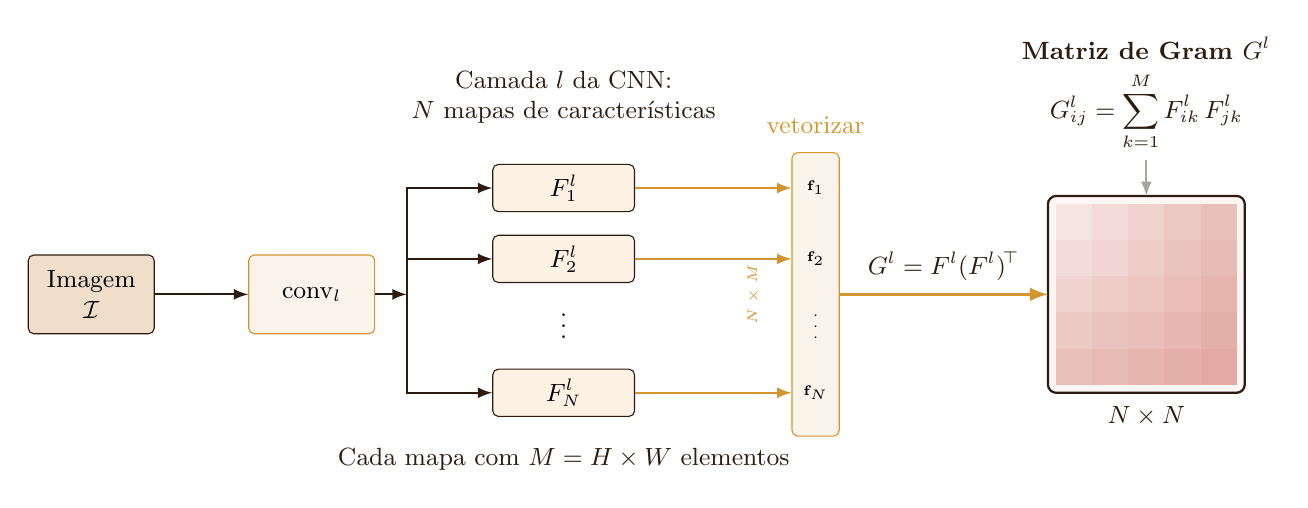
\begin{tikzpicture}[
    >=latex,
    box/.style={draw=wp-text, fill=wp-light, rounded corners=2pt, 
                minimum width=1.6cm, minimum height=1.0cm, 
                align=center, font=\small},
    fm/.style={draw=wp-text, fill=wp-code, rounded corners=2pt, 
               minimum width=1.8cm, minimum height=0.6cm, 
               align=center, font=\small},
    conn/.style={->, draw=wp-text, thick},
    label/.style={font=\small, text=wp-primary}
]

% =========================================================================
% ENTRADA E CAMADA CNN
% =========================================================================
\node[box] (img) at (0, 0) {Imagem\\$\mathcal{I}$};
\node[box, draw=wp-accent, fill=wp-accent!10] (cnn) at (2.8, 0) {conv$_l$};
\draw[conn] (img) -- (cnn);

% =========================================================================
% MAPAS DE CARACTERÍSTICAS
% =========================================================================
\node[fm] (fm1) at (6.0,  1.35) {$F^l_1$};
\node[fm] (fm2) at (6.0,  0.45) {$F^l_2$};
\node[font=\small] at (6.0, -0.30) {$\vdots$};
\node[fm] (fmN) at (6.0, -1.25) {$F^l_{N}$};

\coordinate (branch) at ($(cnn.east) + (0.4, 0)$);
\draw[conn] (cnn.east) -- (branch);
\draw[conn] (branch) |- (fm1.west);
\draw[conn] (branch) |- (fm2.west);
\draw[conn] (branch) |- (fmN.west);


\node[label, text=wp-text, font=\small, align=center] at (6.0, -2.1) 
    {Cada mapa com $M = H \times W$ elementos};

\node[font=\small, text=wp-text, align=center] at (6.0, 2.5) 
    {Camada $l$ da CNN:\\$N$ mapas de características};

% =========================================================================
% MATRIZ VETORIZADA F^l
% =========================================================================
\node[draw=wp-accent, fill=wp-accent!10, rounded corners=2pt, 
      minimum width=0.6cm, minimum height=3.6cm] (matrix_F) at (9.2, 0.0) {};

\node[font=\tiny] at (9.2,  1.35) {$\mathbf{f}_1$};
\node[font=\tiny] at (9.2,  0.45) {$\mathbf{f}_2$};
\node[font=\tiny] at (9.2, -0.30) {$\vdots$};
\node[font=\tiny] at (9.2, -1.25) {$\mathbf{f}_N$};

\draw[conn, draw=wp-accent] (fm1.east) -- (matrix_F.west |- fm1);
\draw[conn, draw=wp-accent] (fm2.east) -- (matrix_F.west |- fm2);
\draw[conn, draw=wp-accent] (fmN.east) -- (matrix_F.west |- fmN);

\node[label, text=wp-accent, font=\small, above=3pt] at (matrix_F.north) {vetorizar};
\node[font=\tiny, text=wp-accent, rotate=90, anchor=south] at ([xshift=-8pt]matrix_F.west) {$N \times M$};

% =========================================================================
% HEATMAP (desenhado diretamente — sem tikzpicture aninhado)
% =========================================================================
\def\cs{0.46}  % tamanho da célula
\def\gn{5}     % grade 5×5
\pgfmathsetmacro{\totalW}{\gn*\cs}
\pgfmathsetmacro{\gramX}{13.4 - \totalW/2}
\pgfmathsetmacro{\gramY}{0.0 + \totalW/2}

% Fundo arredondado
\fill[wp-primary!5, rounded corners=3pt] 
    (\gramX-0.1, \gramY+0.1) rectangle (\gramX+\totalW+0.1, \gramY-\totalW-0.1);

% Células com padrão simétrico
\foreach \i in {0,...,4}{
    \foreach \j in {0,...,4}{
        \pgfmathtruncatemacro{\val}{15 + abs(\i-\j)*5 + min(\i,\j)*8}
        \fill[wp-primary!\val] 
            (\gramX+\i*\cs, \gramY-\j*\cs) rectangle ++(\cs, -\cs);
    }
}

% Borda
\draw[wp-text, thick, rounded corners=3pt] 
    (\gramX-0.1, \gramY+0.1) rectangle (\gramX+\totalW+0.1, \gramY-\totalW-0.1);

% Dimensão
\node[wp-text, font=\small, anchor=north] at (\gramX+\totalW/2, \gramY-\totalW-0.15) {$N \times N$};

% Âncoras nomeadas para conexões
\coordinate (gramWest) at (\gramX-0.1, \gramY-\totalW/2);
\coordinate (gramNorth) at (\gramX+\totalW/2, \gramY+0.1);

% =========================================================================
% SETA DO PRODUTO MATRICIAL
% =========================================================================
\draw[conn, very thick, draw=wp-accent] 
    (matrix_F.east) -- 
    node[above, font=\small, text=wp-text, yshift=1pt] {$G^l = F^l (F^l)^{\!\top}$} 
    (gramWest);

% =========================================================================
% EQUAÇÃO
% =========================================================================
\node[font=\small, text=wp-text, align=center] (eq) at (\gramX+\totalW/2, \gramY+1.4) {
    \textbf{Matriz de Gram $G^l$}\\[4pt]
    $G^l_{ij} = \displaystyle\sum_{k=1}^{M} F^l_{ik}\, F^l_{jk}$
};
\draw[->, draw=wp-text!40, thick] (eq.south) -- (gramNorth);

\end{tikzpicture}
}
\caption{Cálculo da Matriz de Gram na camada $l$. Os $N$ mapas de características 
são vetorizados e organizados na matriz $F^l$ de dimensão $N \times M$. O produto 
 $F^l (F^l)^{\!\top}$ gera a matriz de Gram $G^l$ de tamanho $N \times N$, onde cada 
elemento $G^l_{ij}$ mede a correlação entre os mapas $i$ e $j$.}
\label{fig:gram-matrix}
\end{figure*}
\begin{figure*}[htbp]
\centering
\resizebox{\textwidth}{!}{%
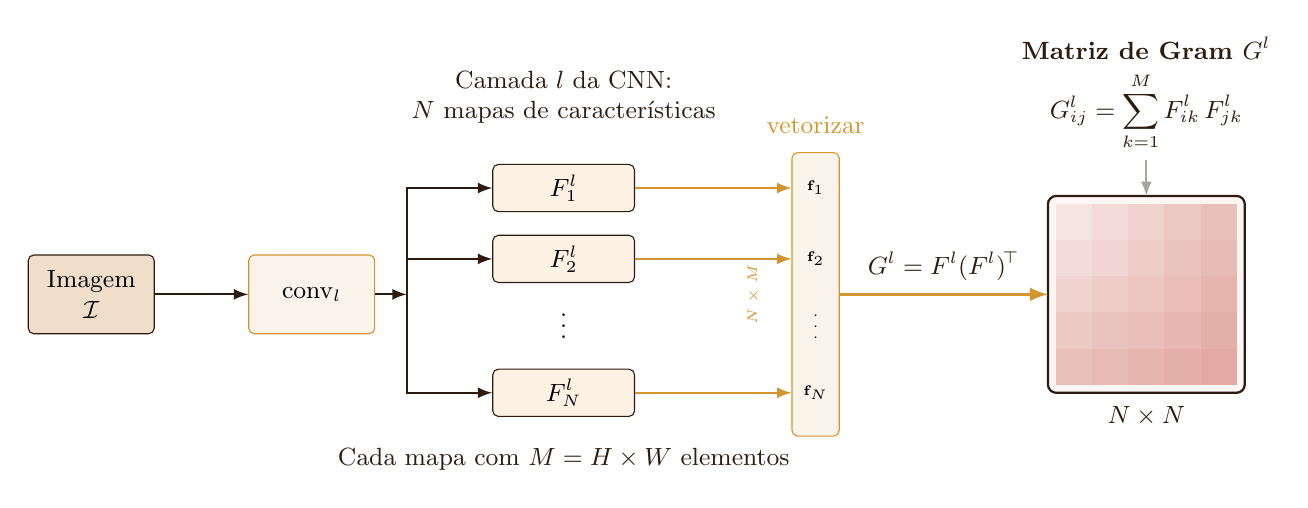
\begin{tikzpicture}[
    >=latex,
    box/.style={draw=wp-text, fill=wp-light, rounded corners=2pt, 
                minimum width=1.6cm, minimum height=1.0cm, 
                align=center, font=\small},
    fm/.style={draw=wp-text, fill=wp-code, rounded corners=2pt, 
               minimum width=1.8cm, minimum height=0.6cm, 
               align=center, font=\small},
    conn/.style={->, draw=wp-text, thick},
    label/.style={font=\small, text=wp-primary}
]

% =========================================================================
% ENTRADA E CAMADA CNN
% =========================================================================
\node[box] (img) at (0, 0) {Imagem\\$\mathcal{I}$};
\node[box, draw=wp-accent, fill=wp-accent!10] (cnn) at (2.8, 0) {conv$_l$};
\draw[conn] (img) -- (cnn);

% =========================================================================
% MAPAS DE CARACTERÍSTICAS
% =========================================================================
\node[fm] (fm1) at (6.0,  1.35) {$F^l_1$};
\node[fm] (fm2) at (6.0,  0.45) {$F^l_2$};
\node[font=\small] at (6.0, -0.30) {$\vdots$};
\node[fm] (fmN) at (6.0, -1.25) {$F^l_{N}$};

\coordinate (branch) at ($(cnn.east) + (0.4, 0)$);
\draw[conn] (cnn.east) -- (branch);
\draw[conn] (branch) |- (fm1.west);
\draw[conn] (branch) |- (fm2.west);
\draw[conn] (branch) |- (fmN.west);


\node[label, text=wp-text, font=\small, align=center] at (6.0, -2.1) 
    {Cada mapa com $M = H \times W$ elementos};

\node[font=\small, text=wp-text, align=center] at (6.0, 2.5) 
    {Camada $l$ da CNN:\\$N$ mapas de características};

% =========================================================================
% MATRIZ VETORIZADA F^l
% =========================================================================
\node[draw=wp-accent, fill=wp-accent!10, rounded corners=2pt, 
      minimum width=0.6cm, minimum height=3.6cm] (matrix_F) at (9.2, 0.0) {};

\node[font=\tiny] at (9.2,  1.35) {$\mathbf{f}_1$};
\node[font=\tiny] at (9.2,  0.45) {$\mathbf{f}_2$};
\node[font=\tiny] at (9.2, -0.30) {$\vdots$};
\node[font=\tiny] at (9.2, -1.25) {$\mathbf{f}_N$};

\draw[conn, draw=wp-accent] (fm1.east) -- (matrix_F.west |- fm1);
\draw[conn, draw=wp-accent] (fm2.east) -- (matrix_F.west |- fm2);
\draw[conn, draw=wp-accent] (fmN.east) -- (matrix_F.west |- fmN);

\node[label, text=wp-accent, font=\small, above=3pt] at (matrix_F.north) {vetorizar};
\node[font=\tiny, text=wp-accent, rotate=90, anchor=south] at ([xshift=-8pt]matrix_F.west) {$N \times M$};

% =========================================================================
% HEATMAP (desenhado diretamente — sem tikzpicture aninhado)
% =========================================================================
\def\cs{0.46}  % tamanho da célula
\def\gn{5}     % grade 5×5
\pgfmathsetmacro{\totalW}{\gn*\cs}
\pgfmathsetmacro{\gramX}{13.4 - \totalW/2}
\pgfmathsetmacro{\gramY}{0.0 + \totalW/2}

% Fundo arredondado
\fill[wp-primary!5, rounded corners=3pt] 
    (\gramX-0.1, \gramY+0.1) rectangle (\gramX+\totalW+0.1, \gramY-\totalW-0.1);

% Células com padrão simétrico
\foreach \i in {0,...,4}{
    \foreach \j in {0,...,4}{
        \pgfmathtruncatemacro{\val}{15 + abs(\i-\j)*5 + min(\i,\j)*8}
        \fill[wp-primary!\val] 
            (\gramX+\i*\cs, \gramY-\j*\cs) rectangle ++(\cs, -\cs);
    }
}

% Borda
\draw[wp-text, thick, rounded corners=3pt] 
    (\gramX-0.1, \gramY+0.1) rectangle (\gramX+\totalW+0.1, \gramY-\totalW-0.1);

% Dimensão
\node[wp-text, font=\small, anchor=north] at (\gramX+\totalW/2, \gramY-\totalW-0.15) {$N \times N$};

% Âncoras nomeadas para conexões
\coordinate (gramWest) at (\gramX-0.1, \gramY-\totalW/2);
\coordinate (gramNorth) at (\gramX+\totalW/2, \gramY+0.1);

% =========================================================================
% SETA DO PRODUTO MATRICIAL
% =========================================================================
\draw[conn, very thick, draw=wp-accent] 
    (matrix_F.east) -- 
    node[above, font=\small, text=wp-text, yshift=1pt] {$G^l = F^l (F^l)^{\!\top}$} 
    (gramWest);

% =========================================================================
% EQUAÇÃO
% =========================================================================
\node[font=\small, text=wp-text, align=center] (eq) at (\gramX+\totalW/2, \gramY+1.4) {
    \textbf{Matriz de Gram $G^l$}\\[4pt]
    $G^l_{ij} = \displaystyle\sum_{k=1}^{M} F^l_{ik}\, F^l_{jk}$
};
\draw[->, draw=wp-text!40, thick] (eq.south) -- (gramNorth);

\end{tikzpicture}
}
\caption{Cálculo da Matriz de Gram na camada $l$. Os $N$ mapas de características 
são vetorizados e organizados na matriz $F^l$ de dimensão $N \times M$. O produto 
 $F^l (F^l)^{\!\top}$ gera a matriz de Gram $G^l$ de tamanho $N \times N$, onde cada 
elemento $G^l_{ij}$ mede a correlação entre os mapas $i$ e $j$.}
\label{fig:gram-matrix}
\end{figure*}
\begin{figure*}[htbp]
\centering
\resizebox{\textwidth}{!}{%
\begin{tikzpicture}[
    >=latex,
    box/.style={draw=wp-text, fill=wp-light, rounded corners=2pt, 
                minimum width=1.6cm, minimum height=1.0cm, 
                align=center, font=\small},
    fm/.style={draw=wp-text, fill=wp-code, rounded corners=2pt, 
               minimum width=1.8cm, minimum height=0.6cm, 
               align=center, font=\small},
    conn/.style={->, draw=wp-text, thick},
    label/.style={font=\small, text=wp-primary}
]

% =========================================================================
% ENTRADA E CAMADA CNN
% =========================================================================
\node[box] (img) at (0, 0) {Imagem\\$\mathcal{I}$};
\node[box, draw=wp-accent, fill=wp-accent!10] (cnn) at (2.8, 0) {conv$_l$};
\draw[conn] (img) -- (cnn);

% =========================================================================
% MAPAS DE CARACTERÍSTICAS
% =========================================================================
\node[fm] (fm1) at (6.0,  1.35) {$F^l_1$};
\node[fm] (fm2) at (6.0,  0.45) {$F^l_2$};
\node[font=\small] at (6.0, -0.30) {$\vdots$};
\node[fm] (fmN) at (6.0, -1.25) {$F^l_{N}$};

\coordinate (branch) at ($(cnn.east) + (0.4, 0)$);
\draw[conn] (cnn.east) -- (branch);
\draw[conn] (branch) |- (fm1.west);
\draw[conn] (branch) |- (fm2.west);
\draw[conn] (branch) |- (fmN.west);


\node[label, text=wp-text, font=\small, align=center] at (6.0, -2.1) 
    {Cada mapa com $M = H \times W$ elementos};

\node[font=\small, text=wp-text, align=center] at (6.0, 2.5) 
    {Camada $l$ da CNN:\\$N$ mapas de características};

% =========================================================================
% MATRIZ VETORIZADA F^l
% =========================================================================
\node[draw=wp-accent, fill=wp-accent!10, rounded corners=2pt, 
      minimum width=0.6cm, minimum height=3.6cm] (matrix_F) at (9.2, 0.0) {};

\node[font=\tiny] at (9.2,  1.35) {$\mathbf{f}_1$};
\node[font=\tiny] at (9.2,  0.45) {$\mathbf{f}_2$};
\node[font=\tiny] at (9.2, -0.30) {$\vdots$};
\node[font=\tiny] at (9.2, -1.25) {$\mathbf{f}_N$};

\draw[conn, draw=wp-accent] (fm1.east) -- (matrix_F.west |- fm1);
\draw[conn, draw=wp-accent] (fm2.east) -- (matrix_F.west |- fm2);
\draw[conn, draw=wp-accent] (fmN.east) -- (matrix_F.west |- fmN);

\node[label, text=wp-accent, font=\small, above=3pt] at (matrix_F.north) {vetorizar};
\node[font=\tiny, text=wp-accent, rotate=90, anchor=south] at ([xshift=-8pt]matrix_F.west) {$N \times M$};

% =========================================================================
% HEATMAP (desenhado diretamente — sem tikzpicture aninhado)
% =========================================================================
\def\cs{0.46}  % tamanho da célula
\def\gn{5}     % grade 5×5
\pgfmathsetmacro{\totalW}{\gn*\cs}
\pgfmathsetmacro{\gramX}{13.4 - \totalW/2}
\pgfmathsetmacro{\gramY}{0.0 + \totalW/2}

% Fundo arredondado
\fill[wp-primary!5, rounded corners=3pt] 
    (\gramX-0.1, \gramY+0.1) rectangle (\gramX+\totalW+0.1, \gramY-\totalW-0.1);

% Células com padrão simétrico
\foreach \i in {0,...,4}{
    \foreach \j in {0,...,4}{
        \pgfmathtruncatemacro{\val}{15 + abs(\i-\j)*5 + min(\i,\j)*8}
        \fill[wp-primary!\val] 
            (\gramX+\i*\cs, \gramY-\j*\cs) rectangle ++(\cs, -\cs);
    }
}

% Borda
\draw[wp-text, thick, rounded corners=3pt] 
    (\gramX-0.1, \gramY+0.1) rectangle (\gramX+\totalW+0.1, \gramY-\totalW-0.1);

% Dimensão
\node[wp-text, font=\small, anchor=north] at (\gramX+\totalW/2, \gramY-\totalW-0.15) {$N \times N$};

% Âncoras nomeadas para conexões
\coordinate (gramWest) at (\gramX-0.1, \gramY-\totalW/2);
\coordinate (gramNorth) at (\gramX+\totalW/2, \gramY+0.1);

% =========================================================================
% SETA DO PRODUTO MATRICIAL
% =========================================================================
\draw[conn, very thick, draw=wp-accent] 
    (matrix_F.east) -- 
    node[above, font=\small, text=wp-text, yshift=1pt] {$G^l = F^l (F^l)^{\!\top}$} 
    (gramWest);

% =========================================================================
% EQUAÇÃO
% =========================================================================
\node[font=\small, text=wp-text, align=center] (eq) at (\gramX+\totalW/2, \gramY+1.4) {
    \textbf{Matriz de Gram $G^l$}\\[4pt]
    $G^l_{ij} = \displaystyle\sum_{k=1}^{M} F^l_{ik}\, F^l_{jk}$
};
\draw[->, draw=wp-text!40, thick] (eq.south) -- (gramNorth);

\end{tikzpicture}
}
\caption{Cálculo da Matriz de Gram na camada $l$. Os $N$ mapas de características 
são vetorizados e organizados na matriz $F^l$ de dimensão $N \times M$. O produto 
 $F^l (F^l)^{\!\top}$ gera a matriz de Gram $G^l$ de tamanho $N \times N$, onde cada 
elemento $G^l_{ij}$ mede a correlação entre os mapas $i$ e $j$.}
\label{fig:gram-matrix}
\end{figure*}

\subsection{Matrizes de Gram na Função de Perda de Estilo}

A função de perda de estilo na transferência de estilo é calculada usando as matrizes de Gram da imagem de estilo ($S$) e da imagem gerada ($G$). Para uma camada específica $l$, a perda de estilo é definida como o erro quadrático médio entre as matrizes de Gram das duas imagens:

\[
\mathcal{L}_{\text{estilo}}^l (S, G) = \frac{1}{4N_l^2 M_l^2} \sum_{i,j} \left(G^l_{ij}(G) - G^l_{ij}(S)\right)^2
\]

Onde:
\begin{itemize}
    \item $G^l_{ij}(S)$ é o elemento da matriz de Gram para a imagem de estilo.
    \item $G^l_{ij}(G)$ é o elemento da matriz de Gram para a imagem gerada.
    \item $N_l$ é o número de mapas de características na camada $l$.
    \item $M_l$ é a dimensão espacial dos mapas de características na camada $l$.
\end{itemize}

A perda de estilo total é calculada como uma soma ponderada das perdas de estilo em várias camadas $L$:

\[
\mathcal{L}_{\text{estilo}} (S, G, L) = \sum_{l \in L} w_l \cdot \mathcal{L}_{\text{estilo}}^l (S, G)
\]

Onde $w_l$ é o peso atribuído à camada $l$.

\subsection{Exemplo de Cálculo de Matriz de Gram}

Considere um exemplo simplificado em que uma camada $l$ tem $N_l = 3$ mapas de características, cada um com dimensão espacial de $M_l = 2 \times 2 = 4$. Os mapas de características podem ser representados como:

\[
F^l = \begin{bmatrix}
1 & 2 & 3 & 4 \\
2 & 0 & 1 & 3 \\
1 & 1 & 2 & 2
\end{bmatrix}
\]

A matriz de Gram $G^l$ é calculada como:

\[
G^l = F^l \cdot (F^l)^T = \begin{bmatrix}
1 & 2 & 3 & 4 \\
2 & 0 & 1 & 3 \\
1 & 1 & 2 & 2
\end{bmatrix}
\cdot
\begin{bmatrix}
1 & 2 & 1 \\
2 & 0 & 1 \\
3 & 1 & 2 \\
4 & 3 & 2
\end{bmatrix}
= \begin{bmatrix}
30 & 20 & 20 \\
20 & 14 & 13 \\
20 & 13 & 14
\end{bmatrix}
\]

Cada elemento de $G^l$ representa a correlação entre os mapas de características correspondentes.

\subsection{Significância das Matrizes de Gram na Transferência de Estilo}

As matrizes de Gram são essenciais para a transferência de estilo porque fornecem uma maneira de quantificar e comparar a textura e o estilo das imagens. Ao minimizar a diferença entre as matrizes de Gram da imagem de estilo e da imagem gerada, o algoritmo garante que a imagem gerada adote o estilo artístico da imagem de estilo enquanto preserva o conteúdo da imagem de conteúdo.

\newpage

\section{Interpretação de GANs via Teoria de Jogos}

As Generative Adversarial Networks (GANs) podem ser interpretadas como um jogo entre dois jogadores: o gerador ($G$) e o discriminador ($D$). Neste apêndice, exploramos como a teoria de jogos fornece uma estrutura matemática para entender o treinamento e a convergência das GANs, baseando-nos no artigo original de Goodfellow et al. (2014).

\subsection{Jogo Minimax}

O artigo original de Goodfellow et al. (2014) formula o treinamento de GANs como um \textbf{jogo minimax}. \textit{Se o discriminador for ótimo}, este jogo se torna de soma zero. No entanto, na prática, a otimização simultânea das funções de perda do gerador e discriminador geralmente resulta em um jogo de soma não-zero. Apesar disso, o princípio fundamental de competição entre os dois jogadores permanece.

A função de valor $V(G, D)$, que define o "pagamento" do jogo, é expressa como:

\begin{equation*}
    \min_G \max_D V(G, D) = \min_{\theta_g} \max_{\theta_d} \left( \mathbb{E}_{x \sim p_{\text{data}}(x)} \left[ \log D(x) \right] + \mathbb{E}_{z \sim p_z(z)} \left[ \log (1 - D(G(z))) \right] \right)
\end{equation*}

Onde:

% GAN — Jogo Minimax (Superfície de Sela 3D Ampliada + Cortes 1D)
% Uso: % GAN — Jogo Minimax (Superfície de Sela 3D Ampliada + Cortes 1D)
% Uso: % GAN — Jogo Minimax (Superfície de Sela 3D Ampliada + Cortes 1D)
% Uso: \input{resources/gan/gan-minimax.tex}
\begin{figure*}[htbp]
\centering
\resizebox{\textwidth}{!}{%
\begin{tikzpicture}[
    >=latex,
    conn/.style={->, wp-primary, thick},
    tuftebox/.style={draw=wp-light, fill=wp-code, rounded corners=2pt, align=center}
]

% =========================================================================
% ESQUERDA: SUPERFÍCIE DE SELA 3D — V = a(θ_G² − θ_D²) (Escala Ampliada)
% =========================================================================
% MODIFICAÇÃO: Fatores de projeção geométrica aumentados para expandir o gráfico
\pgfmathsetmacro{\sx}{1.15}
\pgfmathsetmacro{\sy}{0.55}
\pgfmathsetmacro{\sz}{0.28}
\pgfmathsetmacro{\amp}{0.25}
\pgfmathsetmacro{\cx}{3.2}
\pgfmathsetmacro{\cy}{3.0}

% --- Malha: linhas ao longo de θ_G (θ_D fixo) ---
\foreach \yy in {-2.0,-1.5,...,2.0} {
    \draw[wp-muted!75] plot[domain=-2.6:2.6, samples=50, smooth]
        ({\cx + \x*\sx - \yy*\sy},
         {\cy - \yy*\sz + \amp*(\x*\x - \yy*\yy)});
}

% --- Malha: linhas ao longo de θ_D (θ_G fixo) ---
\foreach \xx in {-2.0,-1.5,...,2.0} {
    \draw[wp-muted!75] plot[domain=-2.0:2.0, samples=50, smooth, variable=\y]
        ({\cx + \xx*\sx - \y*\sy},
         {\cy - \y*\sz + \amp*(\xx*\xx - \y*\y)});
}

% --- Crista ao longo de θ_D (θ_G = 0): D maximiza ---
\draw[wp-accent, thick] plot[domain=-2.0:2.0, samples=60, smooth, variable=\y]
    ({\cx - \y*\sy}, {\cy - \y*\sz - \amp*\y*\y});

% --- Vale ao longo de θ_G (θ_D = 0): G minimiza ---
\draw[wp-primary, thick] plot[domain=-2.6:2.6, samples=60, smooth]
    ({\cx + \x*\sx}, {\cy + \amp*\x*\x});

% --- Assíntotas no plano base (V = 0 → θ_G = ±θ_D) ---
\draw[wp-muted!30, densely dashed]
    ({\cx - 2.6*\sx - 2.6*\sy}, {\cy + 2.6*\sz}) --
    ({\cx + 2.6*\sx + 2.6*\sy}, {\cy - 2.6*\sz});
\draw[wp-muted!30, densely dashed]
    ({\cx - 2.6*\sx + 2.6*\sy}, {\cy - 2.6*\sz}) --
    ({\cx + 2.6*\sx - 2.6*\sy}, {\cy + 2.6*\sz});

% --- Eixos 3D ---
\draw[->, wp-text, thick] (\cx, \cy) -- ({\cx + 3.2*\sx}, \cy)
    node[right, font=\large] {$\theta_G$};
\draw[->, wp-text, thick] (\cx, \cy) -- ({\cx - 3.0*\sy}, {\cy - 3.0*\sz})
    node[below left, font=\large] {$\theta_D$};
\draw[->, wp-text, thick] (\cx, \cy) -- (\cx, {\cy + 3.2})
    node[above, font=\large] {$V$};

% --- Ponto de sela ---
\fill[wp-primary] (\cx, \cy) circle (0.12);
\node[above right=2pt, font=\small\bfseries, text=wp-text] at (\cx, \cy) {Ponto de Sela};

% --- Seta de D: converge ao longo da crista ---
\pgfmathsetmacro{\dsx}{\cx - 1.6*\sy}
\pgfmathsetmacro{\dsy}{\cy - 1.6*\sz - \amp*2.56}
\draw[->, wp-accent, very thick] (\dsx, \dsy) -- (\cx, \cy);
\node[font=\normalsize\bfseries, text=wp-accent, below left=6pt] at (\dsx, \dsy) {$D$ (max)};

% --- Seta de G: converge ao longo do vale ---
\pgfmathsetmacro{\gsx}{\cx + 1.6*\sx}
\pgfmathsetmacro{\gsy}{\cy + \amp*2.56}
\draw[->, wp-primary, very thick] (\gsx, \gsy) -- (\cx, \cy);
\node[font=\normalsize\bfseries, text=wp-primary, above right=12pt] at (\gsx, \gsy) {$G$ (min)};


% =========================================================================
% DIREITA: CORTES 1D ATRAVÉS DO PONTO DE SELA (Deslocado para dar Respiro)
% =========================================================================
% AJUSTE: shift expandido de 10.5 para 12.5 para acomodar o crescimento do 3D
\begin{scope}[shift={(12.5, 0)}]

\draw[->, wp-text, thick] (0, 0) -- (7, 0) node[right, font=\large] {parâmetro};
\draw[->, wp-text, thick] (0, 0) -- (0, 6.2) node[above, font=\large] {$V(D,\mathcal{G})$};

% Linha de referência no valor de sela
\draw[wp-muted!00, thin] (0.3, 3.0) -- (6.7, 3.0);
\node[font=\tiny, text=wp-muted, anchor=east] at (0.3, 3.15) {$V^*$};

% Corte ao longo de θ_D: côncava ↓ (máximo no ponto de sela)
\draw[wp-primary, very thick] plot[domain=0.5:6.5, samples=80, smooth] ({\x}, {3.0 - 0.32*(\x - 3.5)*(\x - 3.5)});

% Corte ao longo de θ_G: côncava ↑ (mínimo no ponto de sela)
\draw[wp-accent, very thick, densely dashed] plot[domain=0.5:6.5, samples=80, smooth] ({\x}, {3.0 + 0.32*(\x - 3.5)*(\x - 3.5)});

% Ponto de sela
\fill[wp-primary] (3.5, 3.0) circle (0.12);
\node[above right=2pt, font=\large, text=wp-text] at (3.5, 3.0) {sela};

% Marca no eixo
\draw[wp-text] (3.5, -0.08) -- (3.5, 0.08);
\node[font=\tiny, text=wp-text, below] at (3.5, -0.1) {$\theta^*$};

% Setas de otimização
\draw[->, wp-primary!60, thick] (1.8, {3.0 - 0.32*2.89}) -- (3.1, {3.0 - 0.32*0.16});
\draw[->, wp-accent!60, thick] (1.8, {3.0 + 0.32*2.89}) -- (3.1, {3.0 + 0.32*0.16});

% Legenda
\node[wp-primary, font=\normalsize, anchor=west, align=left] at (3.8, 5.0) {corte $\theta_D$ $D$ maximiza};
\node[wp-accent, font=\normalsize, anchor=west, align=left] at (3.8, 1.0) {corte $\theta_G$ $G$ minimiza};

\end{scope}


% =========================================================================
% BASE: EQUAÇÃO MINIMAX (Sincronizada ao novo centro geométrico x=7.8)
% =========================================================================
\node[tuftebox, minimum width=15.0cm, minimum height=1.5cm, inner sep=6pt, anchor=north] at (7.8, -1.2) {
    \Large $\displaystyle \min_G \max_D \; V(D, \mathcal{G})
    = \mathbb{E}_{x \sim p_{\mathrm{data}}}[\log D(x)]
    + \mathbb{E}_{z \sim p_z}[\log(1 - D(G(z)))]$ \\[5pt]
    \normalsize
    $D$ maximiza $V$ \qquad\qquad $G$ minimiza $V$ \qquad\qquad Equilíbrio: $p_g = p_{\mathrm{data}} \Rightarrow D(\mathbf{x}) = \tfrac{1}{2}$
};

\end{tikzpicture}
}
\caption{Treinamento de GANs como jogo minimax de soma zero.
\textbf{Esquerda:} superfície de sela $V(\theta_D, \theta_G)$ com o equilíbrio
de Nash. As setas mostram a convergência --- $D$ ao longo da crista
(maximização) e $G$ ao longo do vale (minimização).
\textbf{Direita:} cortes unidimensionais exibindo máximo local para $D$ e
mínimo local para $G$ no ponto de sela.}
\label{fig:gan-minimax}
\end{figure*}
\begin{figure*}[htbp]
\centering
\resizebox{\textwidth}{!}{%
\begin{tikzpicture}[
    >=latex,
    conn/.style={->, wp-primary, thick},
    tuftebox/.style={draw=wp-light, fill=wp-code, rounded corners=2pt, align=center}
]

% =========================================================================
% ESQUERDA: SUPERFÍCIE DE SELA 3D — V = a(θ_G² − θ_D²) (Escala Ampliada)
% =========================================================================
% MODIFICAÇÃO: Fatores de projeção geométrica aumentados para expandir o gráfico
\pgfmathsetmacro{\sx}{1.15}
\pgfmathsetmacro{\sy}{0.55}
\pgfmathsetmacro{\sz}{0.28}
\pgfmathsetmacro{\amp}{0.25}
\pgfmathsetmacro{\cx}{3.2}
\pgfmathsetmacro{\cy}{3.0}

% --- Malha: linhas ao longo de θ_G (θ_D fixo) ---
\foreach \yy in {-2.0,-1.5,...,2.0} {
    \draw[wp-muted!75] plot[domain=-2.6:2.6, samples=50, smooth]
        ({\cx + \x*\sx - \yy*\sy},
         {\cy - \yy*\sz + \amp*(\x*\x - \yy*\yy)});
}

% --- Malha: linhas ao longo de θ_D (θ_G fixo) ---
\foreach \xx in {-2.0,-1.5,...,2.0} {
    \draw[wp-muted!75] plot[domain=-2.0:2.0, samples=50, smooth, variable=\y]
        ({\cx + \xx*\sx - \y*\sy},
         {\cy - \y*\sz + \amp*(\xx*\xx - \y*\y)});
}

% --- Crista ao longo de θ_D (θ_G = 0): D maximiza ---
\draw[wp-accent, thick] plot[domain=-2.0:2.0, samples=60, smooth, variable=\y]
    ({\cx - \y*\sy}, {\cy - \y*\sz - \amp*\y*\y});

% --- Vale ao longo de θ_G (θ_D = 0): G minimiza ---
\draw[wp-primary, thick] plot[domain=-2.6:2.6, samples=60, smooth]
    ({\cx + \x*\sx}, {\cy + \amp*\x*\x});

% --- Assíntotas no plano base (V = 0 → θ_G = ±θ_D) ---
\draw[wp-muted!30, densely dashed]
    ({\cx - 2.6*\sx - 2.6*\sy}, {\cy + 2.6*\sz}) --
    ({\cx + 2.6*\sx + 2.6*\sy}, {\cy - 2.6*\sz});
\draw[wp-muted!30, densely dashed]
    ({\cx - 2.6*\sx + 2.6*\sy}, {\cy - 2.6*\sz}) --
    ({\cx + 2.6*\sx - 2.6*\sy}, {\cy + 2.6*\sz});

% --- Eixos 3D ---
\draw[->, wp-text, thick] (\cx, \cy) -- ({\cx + 3.2*\sx}, \cy)
    node[right, font=\large] {$\theta_G$};
\draw[->, wp-text, thick] (\cx, \cy) -- ({\cx - 3.0*\sy}, {\cy - 3.0*\sz})
    node[below left, font=\large] {$\theta_D$};
\draw[->, wp-text, thick] (\cx, \cy) -- (\cx, {\cy + 3.2})
    node[above, font=\large] {$V$};

% --- Ponto de sela ---
\fill[wp-primary] (\cx, \cy) circle (0.12);
\node[above right=2pt, font=\small\bfseries, text=wp-text] at (\cx, \cy) {Ponto de Sela};

% --- Seta de D: converge ao longo da crista ---
\pgfmathsetmacro{\dsx}{\cx - 1.6*\sy}
\pgfmathsetmacro{\dsy}{\cy - 1.6*\sz - \amp*2.56}
\draw[->, wp-accent, very thick] (\dsx, \dsy) -- (\cx, \cy);
\node[font=\normalsize\bfseries, text=wp-accent, below left=6pt] at (\dsx, \dsy) {$D$ (max)};

% --- Seta de G: converge ao longo do vale ---
\pgfmathsetmacro{\gsx}{\cx + 1.6*\sx}
\pgfmathsetmacro{\gsy}{\cy + \amp*2.56}
\draw[->, wp-primary, very thick] (\gsx, \gsy) -- (\cx, \cy);
\node[font=\normalsize\bfseries, text=wp-primary, above right=12pt] at (\gsx, \gsy) {$G$ (min)};


% =========================================================================
% DIREITA: CORTES 1D ATRAVÉS DO PONTO DE SELA (Deslocado para dar Respiro)
% =========================================================================
% AJUSTE: shift expandido de 10.5 para 12.5 para acomodar o crescimento do 3D
\begin{scope}[shift={(12.5, 0)}]

\draw[->, wp-text, thick] (0, 0) -- (7, 0) node[right, font=\large] {parâmetro};
\draw[->, wp-text, thick] (0, 0) -- (0, 6.2) node[above, font=\large] {$V(D,\mathcal{G})$};

% Linha de referência no valor de sela
\draw[wp-muted!00, thin] (0.3, 3.0) -- (6.7, 3.0);
\node[font=\tiny, text=wp-muted, anchor=east] at (0.3, 3.15) {$V^*$};

% Corte ao longo de θ_D: côncava ↓ (máximo no ponto de sela)
\draw[wp-primary, very thick] plot[domain=0.5:6.5, samples=80, smooth] ({\x}, {3.0 - 0.32*(\x - 3.5)*(\x - 3.5)});

% Corte ao longo de θ_G: côncava ↑ (mínimo no ponto de sela)
\draw[wp-accent, very thick, densely dashed] plot[domain=0.5:6.5, samples=80, smooth] ({\x}, {3.0 + 0.32*(\x - 3.5)*(\x - 3.5)});

% Ponto de sela
\fill[wp-primary] (3.5, 3.0) circle (0.12);
\node[above right=2pt, font=\large, text=wp-text] at (3.5, 3.0) {sela};

% Marca no eixo
\draw[wp-text] (3.5, -0.08) -- (3.5, 0.08);
\node[font=\tiny, text=wp-text, below] at (3.5, -0.1) {$\theta^*$};

% Setas de otimização
\draw[->, wp-primary!60, thick] (1.8, {3.0 - 0.32*2.89}) -- (3.1, {3.0 - 0.32*0.16});
\draw[->, wp-accent!60, thick] (1.8, {3.0 + 0.32*2.89}) -- (3.1, {3.0 + 0.32*0.16});

% Legenda
\node[wp-primary, font=\normalsize, anchor=west, align=left] at (3.8, 5.0) {corte $\theta_D$ $D$ maximiza};
\node[wp-accent, font=\normalsize, anchor=west, align=left] at (3.8, 1.0) {corte $\theta_G$ $G$ minimiza};

\end{scope}


% =========================================================================
% BASE: EQUAÇÃO MINIMAX (Sincronizada ao novo centro geométrico x=7.8)
% =========================================================================
\node[tuftebox, minimum width=15.0cm, minimum height=1.5cm, inner sep=6pt, anchor=north] at (7.8, -1.2) {
    \Large $\displaystyle \min_G \max_D \; V(D, \mathcal{G})
    = \mathbb{E}_{x \sim p_{\mathrm{data}}}[\log D(x)]
    + \mathbb{E}_{z \sim p_z}[\log(1 - D(G(z)))]$ \\[5pt]
    \normalsize
    $D$ maximiza $V$ \qquad\qquad $G$ minimiza $V$ \qquad\qquad Equilíbrio: $p_g = p_{\mathrm{data}} \Rightarrow D(\mathbf{x}) = \tfrac{1}{2}$
};

\end{tikzpicture}
}
\caption{Treinamento de GANs como jogo minimax de soma zero.
\textbf{Esquerda:} superfície de sela $V(\theta_D, \theta_G)$ com o equilíbrio
de Nash. As setas mostram a convergência --- $D$ ao longo da crista
(maximização) e $G$ ao longo do vale (minimização).
\textbf{Direita:} cortes unidimensionais exibindo máximo local para $D$ e
mínimo local para $G$ no ponto de sela.}
\label{fig:gan-minimax}
\end{figure*}
\begin{figure*}[htbp]
\centering
\resizebox{\textwidth}{!}{%
\begin{tikzpicture}[
    >=latex,
    conn/.style={->, wp-primary, thick},
    tuftebox/.style={draw=wp-light, fill=wp-code, rounded corners=2pt, align=center}
]

% =========================================================================
% ESQUERDA: SUPERFÍCIE DE SELA 3D — V = a(θ_G² − θ_D²) (Escala Ampliada)
% =========================================================================
% MODIFICAÇÃO: Fatores de projeção geométrica aumentados para expandir o gráfico
\pgfmathsetmacro{\sx}{1.15}
\pgfmathsetmacro{\sy}{0.55}
\pgfmathsetmacro{\sz}{0.28}
\pgfmathsetmacro{\amp}{0.25}
\pgfmathsetmacro{\cx}{3.2}
\pgfmathsetmacro{\cy}{3.0}

% --- Malha: linhas ao longo de θ_G (θ_D fixo) ---
\foreach \yy in {-2.0,-1.5,...,2.0} {
    \draw[wp-muted!75] plot[domain=-2.6:2.6, samples=50, smooth]
        ({\cx + \x*\sx - \yy*\sy},
         {\cy - \yy*\sz + \amp*(\x*\x - \yy*\yy)});
}

% --- Malha: linhas ao longo de θ_D (θ_G fixo) ---
\foreach \xx in {-2.0,-1.5,...,2.0} {
    \draw[wp-muted!75] plot[domain=-2.0:2.0, samples=50, smooth, variable=\y]
        ({\cx + \xx*\sx - \y*\sy},
         {\cy - \y*\sz + \amp*(\xx*\xx - \y*\y)});
}

% --- Crista ao longo de θ_D (θ_G = 0): D maximiza ---
\draw[wp-accent, thick] plot[domain=-2.0:2.0, samples=60, smooth, variable=\y]
    ({\cx - \y*\sy}, {\cy - \y*\sz - \amp*\y*\y});

% --- Vale ao longo de θ_G (θ_D = 0): G minimiza ---
\draw[wp-primary, thick] plot[domain=-2.6:2.6, samples=60, smooth]
    ({\cx + \x*\sx}, {\cy + \amp*\x*\x});

% --- Assíntotas no plano base (V = 0 → θ_G = ±θ_D) ---
\draw[wp-muted!30, densely dashed]
    ({\cx - 2.6*\sx - 2.6*\sy}, {\cy + 2.6*\sz}) --
    ({\cx + 2.6*\sx + 2.6*\sy}, {\cy - 2.6*\sz});
\draw[wp-muted!30, densely dashed]
    ({\cx - 2.6*\sx + 2.6*\sy}, {\cy - 2.6*\sz}) --
    ({\cx + 2.6*\sx - 2.6*\sy}, {\cy + 2.6*\sz});

% --- Eixos 3D ---
\draw[->, wp-text, thick] (\cx, \cy) -- ({\cx + 3.2*\sx}, \cy)
    node[right, font=\large] {$\theta_G$};
\draw[->, wp-text, thick] (\cx, \cy) -- ({\cx - 3.0*\sy}, {\cy - 3.0*\sz})
    node[below left, font=\large] {$\theta_D$};
\draw[->, wp-text, thick] (\cx, \cy) -- (\cx, {\cy + 3.2})
    node[above, font=\large] {$V$};

% --- Ponto de sela ---
\fill[wp-primary] (\cx, \cy) circle (0.12);
\node[above right=2pt, font=\small\bfseries, text=wp-text] at (\cx, \cy) {Ponto de Sela};

% --- Seta de D: converge ao longo da crista ---
\pgfmathsetmacro{\dsx}{\cx - 1.6*\sy}
\pgfmathsetmacro{\dsy}{\cy - 1.6*\sz - \amp*2.56}
\draw[->, wp-accent, very thick] (\dsx, \dsy) -- (\cx, \cy);
\node[font=\normalsize\bfseries, text=wp-accent, below left=6pt] at (\dsx, \dsy) {$D$ (max)};

% --- Seta de G: converge ao longo do vale ---
\pgfmathsetmacro{\gsx}{\cx + 1.6*\sx}
\pgfmathsetmacro{\gsy}{\cy + \amp*2.56}
\draw[->, wp-primary, very thick] (\gsx, \gsy) -- (\cx, \cy);
\node[font=\normalsize\bfseries, text=wp-primary, above right=12pt] at (\gsx, \gsy) {$G$ (min)};


% =========================================================================
% DIREITA: CORTES 1D ATRAVÉS DO PONTO DE SELA (Deslocado para dar Respiro)
% =========================================================================
% AJUSTE: shift expandido de 10.5 para 12.5 para acomodar o crescimento do 3D
\begin{scope}[shift={(12.5, 0)}]

\draw[->, wp-text, thick] (0, 0) -- (7, 0) node[right, font=\large] {parâmetro};
\draw[->, wp-text, thick] (0, 0) -- (0, 6.2) node[above, font=\large] {$V(D,\mathcal{G})$};

% Linha de referência no valor de sela
\draw[wp-muted!00, thin] (0.3, 3.0) -- (6.7, 3.0);
\node[font=\tiny, text=wp-muted, anchor=east] at (0.3, 3.15) {$V^*$};

% Corte ao longo de θ_D: côncava ↓ (máximo no ponto de sela)
\draw[wp-primary, very thick] plot[domain=0.5:6.5, samples=80, smooth] ({\x}, {3.0 - 0.32*(\x - 3.5)*(\x - 3.5)});

% Corte ao longo de θ_G: côncava ↑ (mínimo no ponto de sela)
\draw[wp-accent, very thick, densely dashed] plot[domain=0.5:6.5, samples=80, smooth] ({\x}, {3.0 + 0.32*(\x - 3.5)*(\x - 3.5)});

% Ponto de sela
\fill[wp-primary] (3.5, 3.0) circle (0.12);
\node[above right=2pt, font=\large, text=wp-text] at (3.5, 3.0) {sela};

% Marca no eixo
\draw[wp-text] (3.5, -0.08) -- (3.5, 0.08);
\node[font=\tiny, text=wp-text, below] at (3.5, -0.1) {$\theta^*$};

% Setas de otimização
\draw[->, wp-primary!60, thick] (1.8, {3.0 - 0.32*2.89}) -- (3.1, {3.0 - 0.32*0.16});
\draw[->, wp-accent!60, thick] (1.8, {3.0 + 0.32*2.89}) -- (3.1, {3.0 + 0.32*0.16});

% Legenda
\node[wp-primary, font=\normalsize, anchor=west, align=left] at (3.8, 5.0) {corte $\theta_D$ $D$ maximiza};
\node[wp-accent, font=\normalsize, anchor=west, align=left] at (3.8, 1.0) {corte $\theta_G$ $G$ minimiza};

\end{scope}


% =========================================================================
% BASE: EQUAÇÃO MINIMAX (Sincronizada ao novo centro geométrico x=7.8)
% =========================================================================
\node[tuftebox, minimum width=15.0cm, minimum height=1.5cm, inner sep=6pt, anchor=north] at (7.8, -1.2) {
    \Large $\displaystyle \min_G \max_D \; V(D, \mathcal{G})
    = \mathbb{E}_{x \sim p_{\mathrm{data}}}[\log D(x)]
    + \mathbb{E}_{z \sim p_z}[\log(1 - D(G(z)))]$ \\[5pt]
    \normalsize
    $D$ maximiza $V$ \qquad\qquad $G$ minimiza $V$ \qquad\qquad Equilíbrio: $p_g = p_{\mathrm{data}} \Rightarrow D(\mathbf{x}) = \tfrac{1}{2}$
};

\end{tikzpicture}
}
\caption{Treinamento de GANs como jogo minimax de soma zero.
\textbf{Esquerda:} superfície de sela $V(\theta_D, \theta_G)$ com o equilíbrio
de Nash. As setas mostram a convergência --- $D$ ao longo da crista
(maximização) e $G$ ao longo do vale (minimização).
\textbf{Direita:} cortes unidimensionais exibindo máximo local para $D$ e
mínimo local para $G$ no ponto de sela.}
\label{fig:gan-minimax}
\end{figure*}

O objetivo é encontrar um ponto de sela desta função, onde o discriminador maximiza $V(G, D)$ em relação a $\theta_d$ e o gerador minimiza $V(G, D)$ em relação a $\theta_g$.

\subsection{Funções de Perda Individuais e Heurística de Saturação Não Decrescente}

Embora a equação acima represente o objetivo geral, o artigo original define as funções de perda individuais do discriminador e do gerador como:

\begin{equation*}
    J^{(D)}(\theta_d, \theta_g) = - \frac{1}{2} \mathbb{E}_{x \sim p_{\text{data}}(x)} \left[ \log D(x) \right] - \frac{1}{2} \mathbb{E}_{z \sim p_z(z)} \left[ \log (1 - D(G(z))) \right]
\end{equation*}

\begin{equation*}
    J^{(G)}(\theta_d, \theta_g) = - J^{(D)}(\theta_d, \theta_g)
\end{equation*}

No entanto, para lidar com problemas de saturação e gradientes fracos no início do treinamento, o artigo original também propõe uma \textbf{alternativa} à função de perda do gerador, conhecida como \textbf{heurística de saturação não decrescente}:

\begin{equation*}
    J^{(G)}(\theta_d, \theta_g) = - \frac{1}{2} \mathbb{E}_{z \sim p_z(z)} \left[ \log (D(G(z))) \right]
\end{equation*}

Essa modificação fornece gradientes mais fortes para o gerador quando o discriminador rejeita facilmente as amostras geradas.

\subsection{Estratégias dos Jogadores}

Cada jogador (gerador e discriminador) tem uma estratégia que consiste em ajustar seus parâmetros ($\theta_g$ e $\theta_d$, respectivamente) para otimizar sua função objetivo:

\begin{enumerate}
    \item \textbf{Discriminador} ($D$): Escolhe seus parâmetros $\theta_d$ para maximizar $J^{(D)}(\theta_d, \theta_g)$. Isso envolve classificar corretamente os dados reais como reais e os dados falsos como falsos. O discriminador é atualizado usando gradiente ascendente em sua função de perda.
    \item \textbf{Gerador} ($G$): Escolhe seus parâmetros $\theta_g$ para minimizar $J^{(G)}(\theta_d, \theta_g)$, seja usando a formulação original (minimizando a divergência de Jensen-Shannon\sidenote{A divergência de Jensen-Shannon é uma derivação da divergência de Kullback-Leibler, com diferenças sutis como o resultado ser sempre um valor finito. Sua raíz quadrada é chamada de Distância de Jensen-Shannon: a similaridade das distribuição é maior quando a distância for mais próxima à zero.}) ou a heurística de saturação não decrescente. O gerador é atualizado usando algoritmos de otimização baseados em gradiente em sua função de perda.
\end{enumerate}

O treinamento das GANs pode ser visto como um processo iterativo em que os jogadores ajustam suas estratégias em resposta às ações do oponente. O artigo original sugere atualizar o discriminador $k$ vezes para cada atualização do gerador.

\subsection{Equilíbrio de Nash}

Para entender o conceito de Equilíbrio de Nash em GANs, é útil defini-lo formalmente no contexto da teoria de jogos. Considere um jogo com dois jogadores, onde:

\begin{itemize}
    \item $G$ é o gerador, com espaço de estratégias $S_G$ (o conjunto de todas as possíveis distribuições que o gerador pode produzir).
    \item $D$ é o discriminador, com espaço de estratégias $S_D$ (o conjunto de todas as possíveis funções discriminadoras).
    \item $V(G, D)$ é a função de valor (ou payoff) que define o resultado do jogo para cada combinação de estratégias.
\end{itemize}

\textbf{Definição}: Um par de estratégias $(G^*, D^*)$ é um \textbf{Equilíbrio de Nash} se, e somente se, as seguintes condições forem satisfeitas:
\begin{enumerate}
    \item Melhor resposta do discriminador: Para qualquer estratégia alternativa do discriminador $D \in S_D$, temos:
    \begin{equation*}
    V(G^*, D^*) \geq V(G^*, D)
    \end{equation*}
    Isso significa que, dado que o gerador está jogando a estratégia $G^*$, o discriminador não pode obter um resultado melhor do que jogar $D^*$. Em outras palavras, $D^*$ é a melhor resposta do discriminador à estratégia $G^*$.
    \item Melhor resposta do gerador: Para qualquer estratégia alternativa do gerador $G \in S_G$, temos:
    \begin{equation*}
    V(G^*, D^*) \leq V(G, D^*)
    \end{equation*}
    Isso significa que, dado que o discriminador está jogando a estratégia $D^*$, o gerador não pode obter um resultado melhor do que jogar $G^*$. Em outras palavras, $G^*$ é a melhor resposta do gerador à estratégia $D^*$.
\end{enumerate}
    
Em termos matemáticos mais compactos:

Um par de estratégias $(G^*, D^*)$ é um Equilíbrio de Nash se:

\begin{equation*}
V(G^*, D^*) = \max_{D \in S_D} V(G^*, D) = \min_{G \in S_G} V(G, D^*)
\end{equation*}

No equilíbrio de Nash, nenhum jogador tem incentivo para mudar sua estratégia unilateralmente. Qualquer desvio da estratégia de equilíbrio resultará em um resultado pior para o jogador que se desviou, assumindo que o outro jogador permaneça com sua estratégia de equilíbrio.


No contexto das GANs, o equilíbrio de Nash global idealmente ocorre quando:

\begin{itemize}
    \item O gerador $G^*$ produz amostras da distribuição real de dados ($p_g(x) = p_{\text{data}}(x)$).
    \item O discriminador $D^*$ atribui uma probabilidade de 1/2 para todas as entradas ($D^*(x) = 1/2$ para todo $x$), indicando que ele não pode distinguir entre amostras reais e geradas.
\end{itemize} 

Importante:

\begin{itemize}
    \item A existência de um equilíbrio de Nash é garantida em jogos finitos (com um número finito de jogadores e estratégias) pelo Teorema de Nash. No entanto, GANs operam em espaços de estratégias contínuos e de alta dimensão, tornando a análise mais complexa.
    \item A definição acima refere-se ao \textbf{equilíbrio de Nash puro}. Existem também \textbf{equilíbrios de Nash mistos}, onde os jogadores escolhem suas estratégias probabilisticamente.
\end{itemize}
\paragraph{Conexão com a Divergência de Jensen-Shannon (Demonstrado no Artigo Original)}

Quando o discriminador é ótimo, \textbf{minimizar a função de valor} $V(G, D)$ \textbf{é equivalente a minimizar a divergência de Jensen-Shannon (JSD)} entre $p_{\text{data}}$ e $p_g$, conforme a seguinte relação:

\begin{equation*}
V(G, D^*_G) = 2 \cdot D_{JS}(p_{\text{data}} || p_g) - \log 4
\end{equation*}

Isso significa que, sob condições ideais, o treinamento de GANs visa minimizar a JSD, uma medida simétrica de similaridade entre distribuições.
\subsection{Convergência do Treinamento}

Embora o artigo original apresente uma prova teórica de convergência para um algoritmo idealizado, ele também reconhece as dificuldades práticas, como:

\begin{enumerate}
    \item \textbf{Capacidade Limitada dos Modelos}: Redes neurais têm capacidade finita.
    \item \textbf{Otimização Imperfeita}: O discriminador nem sempre atinge seu ótimo na prática.
    \item \textbf{Aproximações da Função de Perda}: A heurística de saturação não decrescente, embora útil, não possui a mesma base teórica que a minimização da JSD.
\end{enumerate}

Esses desafios levam a problemas bem conhecidos no treinamento de GANs:

\begin{itemize}
    \item \textbf{Instabilidade}: A natureza antagônica do jogo pode causar oscilações e dificultar a convergência.
    \item \textbf{Colapso de Modo}: O gerador pode aprender a produzir apenas uma variedade limitada de amostras, perdendo a diversidade da distribuição real.
\end{itemize}

\subsection{Exemplo Matemático Simplificado}

Considere um caso simplificado para ilustrar o conceito de equilíbrio de Nash:

\begin{itemize}
    \item Espaço de dados unidimensional: $x \in \mathbb{R}$.
    \item Distribuição real: $p_{\text{data}}(x) = \mathcal{N}(0, 1)$ (Gaussiana padrão).
    \item Gerador: $G(z) = \theta_g z$, onde $z \sim \mathcal{N}(0, 1)$.
    \item Discriminador: $D(x) = \sigma(\theta_d x)$, onde $\sigma$ é a função sigmoide.
\end{itemize}

Neste cenário, o equilíbrio de Nash ocorre quando $\theta_g = 1$ e $\theta_d = 0$. Isso significa que:
\begin{itemize}
    \item O gerador replica perfeitamente a distribuição real.
    \item O discriminador se torna incapaz de distinguir entre dados reais e falsos, atribuindo uma probabilidade de 0,5 para ambos.
\end{itemize}

\paragraph{Demonstração}

Para um gerador fixo, o discriminador ótimo é:

\begin{equation*}
D^*_G(x) = \frac{p_{\text{data}}(x)}{p_{\text{data}}(x) + p_g(x)} = \frac{\mathcal{N}(x; 0, 1)}{\mathcal{N}(x; 0, 1) + \mathcal{N}(x; 0, \theta_g^2)}
\end{equation*}

No equilíbrio de Nash, $p_g(x) = p_{\text{data}}(x)$, o que implica $\theta_g = 1$. Nesse caso, $D^*_G(x) = 1/2$.

Para encontrar o $\theta_d$ ótimo, pode-se derivar a função de perda do discriminador em relação a $\theta_d$. Substituindo $D(x)$ pela expressão do discriminador ótimo $D^*_G(x)$ e considerando o equilíbrio de Nash ($\theta_g = 1$), onde $p_g(x) = p_{\text{data}}(x)$, a derivada se simplifica e se torna zero quando $\theta_d = 0$. Isso indica que, no equilíbrio, o discriminador se torna uma função constante, atribuindo a probabilidade de 0.5 para qualquer entrada.


Este exemplo é extremamente simplificado e serve apenas para fins ilustrativos. Em casos reais, encontrar o equilíbrio de Nash analiticamente é inviável, e o treinamento de GANs depende de métodos numéricos para aproximá-lo.

\end{document}